%% bare_jrnl.tex
%% V1.4b
%% 2015/08/26
%% by Michael Shell
%% see http://www.michaelshell.org/
%% for current contact information.
%%
%% This is a skeleton file demonstrating the use of IEEEtran.cls
%% (requires IEEEtran.cls version 1.8b or later) with an IEEE
%% journal paper.
%%
%% Support sites:
%% http://www.michaelshell.org/tex/ieeetran/
%% http://www.ctan.org/pkg/ieeetran
%% and
%% http://www.ieee.org/

%%*************************************************************************
%% Legal Notice:
%% This code is offered as-is without any warranty either expressed or
%% implied; without even the implied warranty of MERCHANTABILITY or
%% FITNESS FOR A PARTICULAR PURPOSE! 
%% User assumes all risk.
%% In no event shall the IEEE or any contributor to this code be liable for
%% any damages or losses, including, but not limited to, incidental,
%% consequential, or any other damages, resulting from the use or misuse
%% of any information contained here.
%%
%% All comments are the opinions of their respective authors and are not
%% necessarily endorsed by the IEEE.
%%
%% This work is distributed under the LaTeX Project Public License (LPPL)
%% ( http://www.latex-project.org/ ) version 1.3, and may be freely used,
%% distributed and modified. A copy of the LPPL, version 1.3, is included
%% in the base LaTeX documentation of all distributions of LaTeX released
%% 2003/12/01 or later.
%% Retain all contribution notices and credits.
%% ** Modified files should be clearly indicated as such, including  **
%% ** renaming them and changing author support contact information. **
%%*************************************************************************

% *** Authors should verify (and, if needed, correct) their LaTeX system  ***
% *** with the testflow diagnostic prior to trusting their LaTeX platform ***
% *** with production work. The IEEE's font choices and paper sizes can   ***
% *** trigger bugs that do not appear when using other class files.       ***                          ***
% The testflow support page is at:
% http://www.michaelshell.org/tex/testflow/

\documentclass[journal]{IEEEtran}
%
% If IEEEtran.cls has not been installed into the LaTeX system files,
% manually specify the path to it like:
% \documentclass[journal]{../sty/IEEEtran}

% Some very useful LaTeX packages include:
% (uncomment the ones you want to load)

% *** MISC UTILITY PACKAGES ***
%
%\usepackage{ifpdf}
% Heiko Oberdiek's ifpdf.sty is very useful if you need conditional
% compilation based on whether the output is pdf or dvi.
% usage:
% \ifpdf
%   % pdf code
% \else
%   % dvi code
% \fi
% The latest version of ifpdf.sty can be obtained from:
% http://www.ctan.org/pkg/ifpdf
% Also, note that IEEEtran.cls V1.7 and later provides a builtin
% \ifCLASSINFOpdf conditional that works the same way.
% When switching from latex to pdflatex and vice-versa, the compiler may
% have to be run twice to clear warning/error messages.

% *** CITATION PACKAGES ***
%
\usepackage{cite}
% cite.sty was written by Donald Arseneau
% V1.6 and later of IEEEtran pre-defines the format of the cite.sty package
% \cite{} output to follow that of the IEEE. Loading the cite package will
% result in citation numbers being automatically sorted and properly
% "compressed/ranged". e.g., [1], [9], [2], [7], [5], [6] without using
% cite.sty will become [1], [2], [5]--[7], [9] using cite.sty. cite.sty's
% \cite will automatically add leading space, if needed. Use cite.sty's
% noadjust option (cite.sty V3.8 and later) if you want to turn this off
% such as if a citation ever needs to be enclosed in parenthesis.
% cite.sty is already installed on most LaTeX systems. Be sure and use
% version 5.0 (2009-03-20) and later if using hyperref.sty.
% The latest version can be obtained at:
% http://www.ctan.org/pkg/cite
% The documentation is contained in the cite.sty file itself.

% *** GRAPHICS RELATED PACKAGES ***
%
\usepackage{multirow,makecell}
\newcolumntype{C}[1]{>{\centering\arraybackslash}m{#1}}
\newcolumntype{L}[1]{m{#1}}
\ifCLASSINFOpdf
  \usepackage[pdftex]{graphicx}
  % declare the path(s) where your graphic files are
  % \graphicspath{{../pdf/}{../jpeg/}}
  % and their extensions so you won't have to specify these with
  % every instance of \includegraphics
  % \DeclareGraphicsExtensions{.pdf,.jpeg,.png}
\else
  % or other class option (dvipsone, dvipdf, if not using dvips). graphicx
  % will default to the driver specified in the system graphics.cfg if no
  % driver is specified.
  % \usepackage[dvips]{graphicx}
  % declare the path(s) where your graphic files are
  % \graphicspath{{../eps/}}
  % and their extensions so you won't have to specify these with
  % every instance of \includegraphics
  % \DeclareGraphicsExtensions{.eps}
\fi
% graphicx was written by David Carlisle and Sebastian Rahtz. It is
% required if you want graphics, photos, etc. graphicx.sty is already
% installed on most LaTeX systems. The latest version and documentation
% can be obtained at: 
% http://www.ctan.org/pkg/graphicx
% Another good source of documentation is "Using Imported Graphics in
% LaTeX2e" by Keith Reckdahl which can be found at:
% http://www.ctan.org/pkg/epslatex
%
% latex, and pdflatex in dvi mode, support graphics in encapsulated
% postscript (.eps) format. pdflatex in pdf mode supports graphics
% in .pdf, .jpeg, .png and .mps (metapost) formats. Users should ensure
% that all non-photo figures use a vector format (.eps, .pdf, .mps) and
% not a bitmapped formats (.jpeg, .png). The IEEE frowns on bitmapped formats
% which can result in "jaggedy"/blurry rendering of lines and letters as
% well as large increases in file sizes.
%
% You can find documentation about the pdfTeX application at:
% http://www.tug.org/applications/pdftex

% *** MATH PACKAGES ***
%
\usepackage{amsmath}
\usepackage{amssymb}
% A popular package from the American Mathematical Society that provides
% many useful and powerful commands for dealing with mathematics.
%
% Note that the amsmath package sets \interdisplaylinepenalty to 10000
% thus preventing page breaks from occurring within multiline equations. Use:
%\interdisplaylinepenalty=2500
% after loading amsmath to restore such page breaks as IEEEtran.cls normally
% does. amsmath.sty is already installed on most LaTeX systems. The latest
% version and documentation can be obtained at:
% http://www.ctan.org/pkg/amsmath

% *** SPECIALIZED LIST PACKAGES ***
%
%\usepackage{algorithmic}
% algorithmic.sty was written by Peter Williams and Rogerio Brito.
% This package provides an algorithmic environment fo describing algorithms.
% You can use the algorithmic environment in-text or within a figure
% environment to provide for a floating algorithm. Do NOT use the algorithm
% floating environment provided by algorithm.sty (by the same authors) or
% algorithm2e.sty (by Christophe Fiorio) as the IEEE does not use dedicated
% algorithm float types and packages that provide these will not provide
% correct IEEE style captions. The latest version and documentation of
% algorithmic.sty can be obtained at:
% http://www.ctan.org/pkg/algorithms
% Also of interest may be the (relatively newer and more customizable)
% algorithmicx.sty package by Szasz Janos:
% http://www.ctan.org/pkg/algorithmicx

% *** ALIGNMENT PACKAGES ***
%
%\usepackage{array}
% Frank Mittelbach's and David Carlisle's array.sty patches and improves
% the standard LaTeX2e array and tabular environments to provide better
% appearance and additional user controls. As the default LaTeX2e table
% generation code is lacking to the point of almost being broken with
% respect to the quality of the end results, all users are strongly
% advised to use an enhanced (at the very least that provided by array.sty)
% set of table tools. array.sty is already installed on most systems. The
% latest version and documentation can be obtained at:
% http://www.ctan.org/pkg/array

% IEEEtran contains the IEEEeqnarray family of commands that can be used to
% generate multiline equations as well as matrices, tables, etc., of high
% quality.

% *** SUBFIGURE PACKAGES ***
\usepackage{subfigure}
%\ifCLASSOPTIONcompsoc
%  \usepackage[caption=false,font=normalsize,labelfont=sf,textfont=sf]{subfig}
%\else
%  \usepackage[caption=false,font=footnotesize]{subfig}
%\fi
% subfig.sty, written by Steven Douglas Cochran, is the modern replacement
% for subfigure.sty, the latter of which is no longer maintained and is
% incompatible with some LaTeX packages including fixltx2e. However,
% subfig.sty requires and automatically loads Axel Sommerfeldt's caption.sty
% which will override IEEEtran.cls' handling of captions and this will result
% in non-IEEE style figure/table captions. To prevent this problem, be sure
% and invoke subfig.sty's "caption=false" package option (available since
% subfig.sty version 1.3, 2005/06/28) as this is will preserve IEEEtran.cls
% handling of captions.
% Note that the Computer Society format requires a larger sans serif font
% than the serif footnote size font used in traditional IEEE formatting
% and thus the need to invoke different subfig.sty package options depending
% on whether compsoc mode has been enabled.
%
% The latest version and documentation of subfig.sty can be obtained at:
% http://www.ctan.org/pkg/subfig

% *** FLOAT PACKAGES ***
%
%\usepackage{fixltx2e}
% fixltx2e, the successor to the earlier fix2col.sty, was written by
% Frank Mittelbach and David Carlisle. This package corrects a few problems
% in the LaTeX2e kernel, the most notable of which is that in current
% LaTeX2e releases, the ordering of single and double column floats is not
% guaranteed to be preserved. Thus, an unpatched LaTeX2e can allow a
% single column figure to be placed prior to an earlier double column
% figure.
% Be aware that LaTeX2e kernels dated 2015 and later have fixltx2e.sty's
% corrections already built into the system in which case a warning will
% be issued if an attempt is made to load fixltx2e.sty as it is no longer
% needed.
% The latest version and documentation can be found at:
% http://www.ctan.org/pkg/fixltx2e

%\usepackage{stfloats}
% stfloats.sty was written by Sigitas Tolusis. This package gives LaTeX2e
% the ability to do double column floats at the bottom of the page as well
% as the top. (e.g., "\begin{figure*}[!b]" is not normally possible in
% LaTeX2e). It also provides a command:
%\fnbelowfloat
% to enable the placement of footnotes below bottom floats (the standard
% LaTeX2e kernel puts them above bottom floats). This is an invasive package
% which rewrites many portions of the LaTeX2e float routines. It may not work
% with other packages that modify the LaTeX2e float routines. The latest
% version and documentation can be obtained at:
% http://www.ctan.org/pkg/stfloats
% Do not use the stfloats baselinefloat ability as the IEEE does not allow
% \baselineskip to stretch. Authors submitting work to the IEEE should note
% that the IEEE rarely uses double column equations and that authors should try
% to avoid such use. Do not be tempted to use the cuted.sty or midfloat.sty
% packages (also by Sigitas Tolusis) as the IEEE does not format its papers in
% such ways.
% Do not attempt to use stfloats with fixltx2e as they are incompatible.
% Instead, use Morten Hogholm'a dblfloatfix which combines the features
% of both fixltx2e and stfloats:
%
% \usepackage{dblfloatfix}
% The latest version can be found at:
% http://www.ctan.org/pkg/dblfloatfix

%\ifCLASSOPTIONcaptionsoff
%  \usepackage[nomarkers]{endfloat}
% \let\MYoriglatexcaption\caption
% \renewcommand{\caption}[2][\relax]{\MYoriglatexcaption[#2]{#2}}
%\fi
% endfloat.sty was written by James Darrell McCauley, Jeff Goldberg and 
% Axel Sommerfeldt. This package may be useful when used in conjunction with 
% IEEEtran.cls'  captionsoff option. Some IEEE journals/societies require that
% submissions have lists of figures/tables at the end of the paper and that
% figures/tables without any captions are placed on a page by themselves at
% the end of the document. If needed, the draftcls IEEEtran class option or
% \CLASSINPUTbaselinestretch interface can be used to increase the line
% spacing as well. Be sure and use the nomarkers option of endfloat to
% prevent endfloat from "marking" where the figures would have been placed
% in the text. The two hack lines of code above are a slight modification of
% that suggested by in the endfloat docs (section 8.4.1) to ensure that
% the full captions always appear in the list of figures/tables - even if
% the user used the short optional argument of \caption[]{}.
% IEEE papers do not typically make use of \caption[]'s optional argument,
% so this should not be an issue. A similar trick can be used to disable
% captions of packages such as subfig.sty that lack options to turn off
% the subcaptions:
% For subfig.sty:
% \let\MYorigsubfloat\subfloat
% \renewcommand{\subfloat}[2][\relax]{\MYorigsubfloat[]{#2}}
% However, the above trick will not work if both optional arguments of
% the \subfloat command are used. Furthermore, there needs to be a
% description of each subfigure *somewhere* and endfloat does not add
% subfigure captions to its list of figures. Thus, the best approach is to
% avoid the use of subfigure captions (many IEEE journals avoid them anyway)
% and instead reference/explain all the subfigures within the main caption.
% The latest version of endfloat.sty and its documentation can obtained at:
% http://www.ctan.org/pkg/endfloat
%
% The IEEEtran \ifCLASSOPTIONcaptionsoff conditional can also be used
% later in the document, say, to conditionally put the References on a 
% page by themselves.

% *** PDF, URL AND HYPERLINK PACKAGES ***
%
\usepackage{url}
% url.sty was written by Donald Arseneau. It provides better support for
% handling and breaking URLs. url.sty is already installed on most LaTeX
% systems. The latest version and documentation can be obtained at:
% http://www.ctan.org/pkg/url
% Basically, \url{my_url_here}.

\usepackage{orcidlink}

% *** Do not adjust lengths that control margins, column widths, etc. ***
% *** Do not use packages that alter fonts (such as pslatex).         ***
% There should be no need to do such things with IEEEtran.cls V1.6 and later.
% (Unless specifically asked to do so by the journal or conference you plan
% to submit to, of course. )

% correct bad hyphenation here
\hyphenation{intercon-nected mean-ingful net-works Neverthe-less inad-vertent Manage-ment in-formation individu-ally trans-mission modi-fications}

\begin{document}
%
% paper title
% Titles are generally capitalized except for words such as a, an, and, as,
% at, but, by, for, in, nor, of, on, or, the, to and up, which are usually
% not capitalized unless they are the first or last word of the title.
% Linebreaks \\ can be used within to get better formatting as desired.
% Do not put math or special symbols in the title.
\title{Content Storage Management and Precaching Scheme in Content-Centric Networks-based Internet of Vehicle}
%
%
% author names and IEEE memberships
% note positions of commas and nonbreaking spaces ( ~ ) LaTeX will not break
% a structure at a ~ so this keeps an author's name from being broken across
% two lines.
% use \thanks{} to gain access to the first footnote area
% a separate \thanks must be used for each paragraph as LaTeX2e's \thanks
% was not built to handle multiple paragraphs
%

\newcommand{\orcidauthorA}{0000-0003-3971-0715} % Youngju Nam
\newcommand{\orcidauthorB}{0000-0001-9410-7244} % Hyunseok Choi
\newcommand{\orcidauthorC}{0000-0002-0422-0647} % Euisin Lee

\author{Youngju Nam,
        Hyeonseok Choi,
        and Euisin Lee%,~\IEEEmembership{Life~Fellow,~IEEE}% <-this % stops a space

\thanks{Manuscript received April 00, 2024; revised August 00, 2024.
This work was supported by a National Research Foundation of Korea (NRF) grant funded by the Korean government (Ministry of Science and ICT (MSIT)) (No. 2022R1A2C1010121).
This research was supported by Basic Science Research Program through the National Research Foundation of Korea(NRF) funded by the Ministry of Education(RS-2023-00272850)\textit{(Corresponding author: Euisin Lee.)}}
\thanks{Euisin Lee is with the School of Information and Communication Engineering, Chungbuk National University, Cheongju, Republic of Korea (e-mail: eslee@chungbuk.ac.kr).}% <-this % stops a space
\thanks{Hyeonseok Choi is with Research Institute for Computer and Information Communication, Chungbuk National University, Cheongju 28644, Republic of Korea (e-mail: hschoi@chungbuk.ac.kr).}
\thanks{Youngju Nam is with the School of Software, Kunsan National University, Gunsan 54150, Republic of Korea (e-mail: imnyj@kunsan.ac.kr).}
\thanks{Digital Object Identifier 10.0000/JIOT.2024.0000000}}

% note the % following the last \IEEEmembership and also \thanks - 
% these prevent an unwanted space from occurring between the last author name
% and the end of the author line. i.e., if you had this:
% 
% \author{....lastname \thanks{...} \thanks{...} }
%                     ^------------^------------^----Do not want these spaces!
%
% a space would be appended to the last name and could cause every name on that
% line to be shifted left slightly. This is one of those "LaTeX things". For
% instance, "\textbf{A} \textbf{B}" will typeset as "A B" not "AB". To get
% "AB" then you have to do: "\textbf{A}\textbf{B}"
% \thanks is no different in this regard, so shield the last } of each \thanks
% that ends a line with a % and do not let a space in before the next \thanks.
% Spaces after \IEEEmembership other than the last one are OK (and needed) as
% you are supposed to have spaces between the names. For what it is worth,
% this is a minor point as most people would not even notice if the said evil
% space somehow managed to creep in.

% The paper headers
\markboth{IEEE INTERNET OF THINGS JOURNAL,~Vol.~00, No.~0, August~2024}%
{Youngju Nam \MakeLowercase{\textit{et al.}}: Content Storage Management and Precaching Scheme using caching priority algorithm in CCN-IoV}
% The only time the second header will appear is for the odd numbered pages
% after the title page when using the twoside option.
% 
% *** Note that you probably will NOT want to include the author's ***
% *** name in the headers of peer review papers.                   ***
% You can use \ifCLASSOPTIONpeerreview for conditional compilation here if
% you desire.

% If you want to put a publisher's ID mark on the page you can do it like
% this:
%\IEEEpubid{0000--0000/00\$00.00~\copyright~2015 IEEE}
% Remember, if you use this you must call \IEEEpubidadjcol in the second
% column for its text to clear the IEEEpubid mark.

% use for special paper notices
%\IEEEspecialpapernotice{(Invited Paper)}

% make the title area
\maketitle

% As a general rule, do not put math, special symbols or citations
% in the abstract or keywords.
\begin{abstract}
The emergence of smart cars has led to a significant increase in mobile data traffic on the backhaul links as a vast amount of contents is generated and consumed in the Internet of Vehicles (IoVs).
To cope with this situation, the precaching research of content-centric networks (CCN) has been applied as a promising solution for reducing traffic consumption.
However, most precaching schemes in CCN-IoVs only focus on delay-sensitive content and don't have proper content storage management, limiting their ability to minimize delays.
To address these issues, we thus propose a novel content storage management and precaching (CSMP) scheme consisting of three methods.
To prevent the erases of precached or popular content, we have designed a content storage management method based on our caching priority algorithm.
Additionally, we have designed a delay-sensitive content precaching method to improve mobility prediction and reduce delays using the recalculation time based on Gaussian distribution with skewness.
Finally, we have designed a delay-tolerant content precaching method to minimize backhaul link traffic consumption by using an integer linear programming approach.
The proposed CSMP scheme improved the evaluation value considering the success ratio and the backhaul link traffic by 23.21\% compared with the existing schemes in our NS3-based simulations.
\end{abstract}

% Note that keywords are not normally used for peerreview papers.
\begin{IEEEkeywords}
Content-Centric Network, Internet of Vehicle, Precaching, Caching storage management, Delay tolerant/sensitive content, Priority algorithm.
\end{IEEEkeywords}


% For peer review papers, you can put extra information on the cover
% page as needed:
% \ifCLASSOPTIONpeerreview
% \begin{center} \bfseries EDICS Category: 3-BBND \end{center}
% \fi
%
% For peerreview papers, this IEEEtran command inserts a page break and
% creates the second title. It will be ignored for other modes.
\IEEEpeerreviewmaketitle

\section{Introduction}
\IEEEPARstart{T}{he} Internet of Things (IoT) encompasses many interconnected physical and virtual objects, such as smart devices, that collaborate to collect, refine, process, and exchange meaningful information via the public Internet.
These smart devices, which can be assigned unique identities or IP addresses, have the ability to autonomously send and receive data across networks.
When we focus on vehicles within this IoT ecosystem, it evolves into the Internet of Vehicles (IoV).
Smart vehicles equipped with sensors, GPS, and onboard units (OBUs) enable automated driving, providing users with more leisure time to spend more content during their driving journey \cite{Zhe2020, yuan2018}.
This increased demand for content, coupled with the increased size of content due to higher quality displays and improved content quality, results in significant data traffic consumption \cite{Kumer2013, Pranav2019, Reichardt2002, Yen2020}.
Ericsson's Mobility Report predicts that mobile data traffic will triple from 160 $EB$ per month in 2023 to 563 $EB$ per month in 2029, with video traffic constituting a significant portion \cite{Ericsson}.
In addition, due to the mobility of vehicles as users in IoV, the increased size of content also means that a single base station (BS) or roadside unit (RSU) cannot always provide all pieces of the requested content to the requester vehicle within its communication coverage, resulting in access delays during frequent handovers.
Moreover, when multiple vehicles request the same content within the coverage area of a BS or RSU, it creates additional data traffic and delays for re-accessing the content server, leading to congestion, similar to the challenges seen at crowded events, due to the inherent limitations of communication resources in both the BS and RSU.
These problems reduce the quality of service (QoS) for vehicle users who spend their time enjoying various content.

To improve QoS for vehicle users, Content-Centric Networks (CCNs~\cite{Jacobson2009, zhang2014}) have emerged as a promising solution in IoV, called CCN-IoV \cite{Li2017, Hichri2021}.
Different from host-centric networks, CCNs utilize content names instead of IP addresses to identify and cache content in network nodes.
This approach significantly reduces the need to access content servers by downloading content using the name of the content that can be cached in the caching storage of BSs or RSUs during provisioning or forwarding, resulting in reduced access delays and backhaul link traffic.
However, the inherent limitation in caching storage capacity within BSs and RSUs prevents the caching of all content.
Thus, when a vehicle user requests content that isn't cached at its current BS or RSU, they must access the content server or other RSUs that have cached it, leading to additional accessing delays.
To handle these accessing delays, precaching schemes have been introduced and researched in CCN-IoV \cite{Ding2022, Wu2022, AlNagar2022}.
This scheme proactively caches requested content at the next predicted RSU along the user vehicle's route.
As a result, the accuracy of this prediction is paramount to the performance of precaching.
In numerous studies, the frequent recalculations of predictions have presented a significant computational burden \cite{Yu2022, Xu2020}.
Fortunately, predicting the mobility of a vehicle on roads where speed limits are enforced is much easier than predicting the movement of living entities, such as humans, animals, etc.
Nevertheless, if cached or precached content surpasses the storage capacity of an RSU, older content is deleted, resulting in additional traffic and access delays when requested by other users.
In the worst case, this can lead to the wastage of over double the required traffic.
Additionally, these issues can introduce prolonged delays and buffering for vehicle users while they enjoy their content.
For delay-sensitive applications such as driver assistance systems, these challenges are directly related to user safety, especially at roads of high speeds.


For precaching in CCN-IoV, the design of effective caching storage management is one of the crucial and challenging issues due to the constrained cache size of RSUs and BSs \cite{Wang2021, Lin2021, Yao2018}.
The main factors for this design involve prioritizing content, preventing inadvertent content erasure, and precaching requested content.
Then, efficient methods to solve this issue can improve the hit ratio for content requests of vehicle users, resulting in enhanced network performances, including reduced delay and traffic consumption.
Despite its importance, existing precaching schemes (e.g. \cite{Wang2021, Feng2023}) often focus on content popularity and overlook a critical factor, particularly the neglect of delay-tolerant content (DTC) in CCN-IoV.
This neglect can lead to unnecessary backhaul link traffic, increased computing resource consumption, and higher storage costs.
Some studies propose schemes that intelligently manage node storage by predicting content requests based on vehicle mobility and content popularity \cite{Zhe2020, Liu2018}.
These schemes divide precaching into proactive caching of popular content and proactive caching of requested content based on the prediction of the next RSU encounter.
However, existing schemes may lack prioritization, leading to additional traffic and decreased efficiency.
Furthermore, without considering delay-tolerant content, RSUs result in wasteful traffic and storage costs for reckless precaching.
Thus, a novel caching storage management approach, considering DTC, is imperative to optimize the network performance of precaching in CCN-IoV.

Therefore, to enhance the efficiency of precaching in CCN-IoV, we propose a Content Storage Management and Precaching (CSMP) scheme consisting of three methods: the Content Storage Management (CSM) method to set the priority of the precached or cached content; the Delay Sensitive Content Precaching (DSCP) method that conducts recalculation to improve the prediction accuracy by updating a vehicle's mobility information; the Delay-Tolerant Content Precaching (DTCP) method with considering tolerable delay of the DTC.
First, we design the CSM method to establish cache modes and to set caching priority values according to modes in order to prevent the inadvertent removal of the content that is likely to be requested.
Subsequently, to account for mobility changes in vehicles for prediction to precache delay-sensitive content (DSC), we mathematically design a prediction model to calculate the recalculation time in our DSCP method.
Our prediction model for precaching DSC not only relies on Gaussian distribution but also incorporates skewness for enhanced prediction accuracy.
Moreover, we design the DTCP method to utilize the cached RSUs by considering the tolerable delay of the requested DTC in order to reduce backhaul link traffic.
This consideration of tolerable delay ensures the completion of providing delay-tolerant content to the requester vehicle within the tolerable delay.
Simultaneously, to reflect vehicles' requests for various content, we make a content request model based on Poisson distribution, Zipf's law, and Gaussian distribution.
To evaluate the efficiency of our scheme comprehensively, we design a Manhattan-based mobility model incorporating speed with Gaussian distribution and skewness.
Through simulation results conducted in various network environments, we validate our scheme's performance enhancement in terms of minimizing traffic consumption on backhaul links, reducing storage costs, and mitigating repeated requests and computation overhead in prediction processes.

The remainder of this paper is organized as follows.
Related work is reviewed in Section \ref{sec.rw}.
In Section \ref{sec.nm}, we describe the network model of the proposed CSMP scheme.
Then, we introduce the CSMP scheme and propose our three methods: the CSM method, the DSCP method, and the DTCP method in Section \ref{sec.csmp}.
We present the performance evaluation and results analysis in Section \ref{sec.perf}.
Finally, Section \ref{sec.conc} concludes this paper.


\section{Related Work} \label{sec.rw}
In the current IoV paradigm, content download faces significant challenges as routing is traditionally based on IP addresses, and vehicles often operate at high speeds.
When multiple vehicles within the coverage area of a Roadside Unit (RSU) request the same content, the conventional IP address-based routing results in each request being individually resolved through connections between the content server and the RSU where the vehicles are located.
This method incurs more than double the necessary traffic on backhaul links.
Moreover, the frequent handovers driven by the high speeds of vehicles contribute to access delays, as each new RSU's coverage area triggers a request to the content server.
Furthermore, the download of content from the server over long-distance connections not only leads to access delays for vehicle users but also contributes to increased traffic consumption on backhaul links.


\subsection{CCN-IoV}
In response to challenges within vehicular networks, researchers have delved into the realm of Content-Centric Networks (CCNs)~\cite{Amadeo2012, Su2017, Wang2019}.
The integration of CCNs into the Internet of Vehicles (IoV) presents a paradigm shift, alleviating delays and reducing traffic consumption by prioritizing content based on its name rather than relying on IP addresses for location.
Embodying the principles of CCNs, all nodes within the IoV architecture are furnished with storage devices to cache the forwarded or provided content.
Therefore, in an IoV framework integrated with CCNs, every RSU is equipped with a dedicated storage device, fostering an environment that efficiently harnesses the advantages of CCNs.
\cite{Amadeo2012} postulated that adopting a CCN strategy could surpass the traditional TCP/IP protocol suite, adeptly managing the dynamic, brief, and sporadic connections prevalent in vehicular environments.
A comprehensive simulation study was undertaken to evaluate the performance of the proposed content-centric vehicular networking architecture across diverse traffic loads, vehicle densities, and content popularity scenarios, assessing both its efficacy and efficiency.
\cite{Su2017} introduced an innovative content-centric vehicular network (CCVN) framework, unveiling an integrated algorithm for delivering content to vehicles through content-centric units.
These units facilitated content storage based on the priorities that are determined by content popularity and vehicle density.
The incorporation of a content-centric unit in their CCVN enabled the management of exchanged content between vehicles based on naming information, with pending interests regularly updated through analysis of transmission ratios and network topology.
\cite{Wang2019} introduced an IP-based framework for vehicular content-centric networking, emphasizing content acquisition based on specific positions.
The framework allowed requesters to acquire content in an address-centric unicast manner, ensuring the return of content to the requester without relying on reverse paths.
Additionally, the framework facilitated content retrieval from the closest provider at a given position, effectively reducing costs associated with content acquisition.
% limits of basic CCN-IoV
However, despite these advancements, a formidable challenge persists in the finite storage capacity of each node.
This constraint impedes RSUs from caching all content, leading to complications when a vehicle requests content that is not cached in the RSU's storage.
This challenge of limited storage capacity and the associated consequences for content availability and access forms a critical issue within the domain of CCN-applied IoV.
It underscores the necessity for innovative solutions to optimize storage management, enhance content accessibility, and elevate the overall efficiency of vehicular networks.


\begin{table*}
    \caption{The summary of the related works on precaching in CCN-IoV}
    \begin{tabular}{C{0.05\textwidth}|C{0.05\textwidth}|C{0.1\textwidth}|C{0.1\textwidth}|C{0.05\textwidth}|L{0.5\textwidth}} % total: 15.5 cm
        \hline
        \hline
        \textbf{Index} & \textbf{Purpose} & \textbf{Prediction matrix} & \textbf{Caching priority} & \textbf{DTC} & \multicolumn{1}{c}{\textbf{Description}} \\
        \hline
        \hline
        \cite{Ostrovskaya2018} & hit ratio & freshness, popularity, distance & Least Recently Used & X & 
                A scheme for proactively replacing content by presenting metrics in two ways, taking into account the freshness and popularity of the content and the distance from the content server.\\
        \hline
        \cite{Amadeo2021} & delay, traffic & popularity, availability & popularity, lifetime & X & 
                A novel distributed caching strategy that distributively caches the content based on its popularity, residual lifetime, and the perceived availability of the same content in the neighborhood before being requested, leading to reducing the network traffic load and content retrieval time.\\
        \hline
        \cite{Dua2019} & traffic & popularity & popularity & X & 
                A Hierarchical Hybrid Content Delivery scheme using Bloom Filter (H2CDBF) and a learning automata-based cache update policy based on content popularity prediction to alleviate traffic congestion by addressing the challenges of efficient content sharing and high mobility in vehicular networks. \\
        \hline
        \cite{Ikram2021} & mobility support & mobility & popularity & X & 
                A new proactive caching strategy for Vehicular Ad-hoc Networks (VANETs) to provide mobility support by precaching the requested content to the next RSU, taking into account vehicle mobility in the left, right, and straight ahead directions at an intersection.\\
        \hline
        \cite{Zhe2020} & delay, traffic & popularity, mobility & request probability & X & 
                A novel hierarchical proactive caching approach based on the non-negative matrix factorization technique, which considers both the user's future demands and vehicle mobility to minimize delays and the network load.\\
        \hline
        \cite{Liu2018} & traffic & popularity, mobility & request probability & X & 
                 A mobility-aware video precaching and replacement strategies that precache and replace chunks based on vehicle mobility and its popularity by formulating the optimization problem as an integer linear programming at every time slot to alleviate the load of the core network. \\
        \hline
        \cite{Grewe2018} & mobility support & hops, popularity & freshness & X & 
                An adaptive decentralized prefetching mechanism that replaces the outdated content and precaches the popular and low-cost content to provide the mobility support service for ICNs in vehicular scenarios. \\
        \hline
        \cite{Qi2017} & reliability, traffic & mobility & X & O & 
                A novel message routing scheme by the timeliness-aware trajectory data mining algorithm based on the prediction of vehicles' future RSU entrances in VANETs that enable delay-tolerant networks. \\
        \hline
        \cite{Xia2020} & delay & mobility & reliability & O & 
                A new delay-tolerant data transmission architecture that integrates cloud computing, fog computing, software-defined network, and other technologies to solve high transmission latency problems in IoV\\
        \hline
        \hline    
    \end{tabular}
    \label{tab:mob}
\end{table*}


\subsection{Precaching scheme in IoV}
To address the intricacies of CCNs in the context of the IoV, the development of the precaching scheme has emerged as a promising solution \cite{Ostrovskaya2018, Amadeo2021, Dua2019, Park2019, Ahani2018, AlNagar2019, Liang2018}.
This scheme aims to proactively cache content, considering two primary strategies: popularity-based precaching and mobility-based precaching.
Popularity-based precaching is the precaching scheme that RSUs precache popular content because it is more likely to be requested.
\cite{Ostrovskaya2018} introduced the multi-metric content replacement policy (M$^{2}$CRP) tailored for content stores in Vehicular Ad-hoc Networks (VANETs) driven by named data networking (NDN).
For enhanced performance in VANET applications, M$^{2}$CRP incorporates three key metrics, which are the freshness of content, its popularity, and the distance between content receipt and storage locations in content stores, relative to the caching node's current location.
\cite{Amadeo2021} proposed the Diversity-Improved Caching of Popular Transient Content (DANTE) strategy.
DANTE empowers vehicles to autonomously decide locally cached content based on factors like content residual lifetime, popularity, and perceived content availability in the vicinity.
DANTE also introduces minor architectural modifications in NDN nodes and packet fields to streamline its operations.
Vehicles make caching decisions independently, enabling the discovery of fresh and popular distinct content without overwhelming the network with requests reaching the original source.
To enhance content distribution efficiency in CCN-IoV, \cite{Dua2019} presented a content caching scheme utilizing a bloom filter model which is based on a probabilistic data structure.
The bloom filter model optimizes time complexity for content insertion, deletion, and search operations, turning vehicles into caches and facilitating cooperative content distribution.
Popularity-based Precaching involves RSUs precaching popular content due to its higher likelihood of being requested.
While this strategy showcases promise, the fundamental challenge arises from the finite storage capacity of RSUs.
The inherent limitation impedes the comprehensive precaching of all popular content, necessitating careful management and prioritization.

In the realm of Mobility-based Precaching, the proactive caching of content is driven by predictions regarding the RSU a requester vehicle will encounter \cite{Ahani2018, AlNagar2019, Liang2018, Ikram2021, Zhe2020, Liu2018, Feng2023, Zhao2023, Khan2024}.
Leveraging trajectory and speed information, the RSU predicted to be encountered precaches the requested content in anticipation of the vehicle's arrival.
However, the efficiency of this approach hinges on the accuracy of mobility predictions.
If inaccuracies occur, leading to unnecessary precaching, it results in wasted backhaul link traffic, diminishing the effectiveness of the strategy.
\cite{Ikram2021} introduced the Left-Right-Front (LRF) cache strategy tailored for precaching in IoV.
The LRF cache strategy proactively caches the requested data at upcoming nodes/RSUs for vehicles within a predefined Information-Centric Networking (ICN) architecture.
Notably, it addresses the challenges posed by the dynamic nature of the network and mobility, characteristic of IoV nodes in an ICN environment.
This strategy significantly enhances cache utilization, hop ratios, and resolved interest ratios.
\cite{Feng2023} aimed to design a novel edge-computing-enabled hierarchical cooperative caching framework. This framework employed a predictive approach, utilizing historical vehicle trajectory data and user requests to anticipate vehicle trajectory and content popularity. The resulting predictions enabled the framework to achieve an effective hit ratio and minimize average delay.
\cite{Zhao2023} proposed a proactive edge computing and caching scheme to optimize task offloading. The proximal policy optimization (PPO) was used to predict which RSU would compute and cache the requested content. This was based on several factors, including the total time delay of the RSU, the total time delay of the vehicle, the expected content popularity, the content caching status, and the traffic status of the RSU. The prediction aimed to optimize both the hit ratio and the total delay, which are in a trade-off relationship.
\cite{Zhe2020} proposed a novel hierarchical proactive caching (i.e. precaching) scheme that factors in both the anticipated demands of autonomous vehicle users and their mobility.
This innovative scheme employs the non-negative matrix factorization (NMF) technique to predict user preferences, subsequently forecasting users' future demands by considering the historical popularity of videos.
The calculation of video chunk numbers for precaching incorporates the user's arrival and departure times at an edge node, contingent on their current velocity vector.
This scheme takes into account both predicted ratings and the prior popularity of videos to effectively anticipate users' future demands.
\cite{Liu2018} presented a novel video prefetch caching and replacement strategy that introduces a mobility-aware utility function.
This function is based on the user's moving probability and the popularity of video clips.
By factoring in network and storage resource costs at each time slice, a unified cache replacement strategy is constructed through prefetching and caching to establish utility functions.
This strategy adeptly quantifies the value of caching and prefetching video properties, leading to improved utility and cache hit rates for unit storage.
The overall outcome ensures the stability of video services, particularly during user cell handover events.
The effectiveness of this strategy was thoroughly evaluated in the taxi trajectory-based scenario.
Furthermore, \cite{Ahani2018, AlNagar2019, Liang2018} optimized the number of chunks that should be precached based on requester vehicles' mobility while considering various constraints such as link capacity, storage, or buffer time.
% limits of mob-based precaching
The challenges extend further to the management of precached and cached content.
Finite storage capacity forces decisions on erasing content under certain conditions.
Efficiently managing the lifecycle of cached content is critical, involving considerations of when to erase content to optimize space while ensuring that relevant and frequently requested content remains accessible.
Moreover, the frequent recalculations necessary for prediction in Mobility-based Precaching present a computational burden, impacting the system's overall efficiency and responsiveness.
Striking a balance between recalculation frequency and compute resource consumption becomes critical to maintaining optimal performance.
In essence, the challenges within the precaching scheme in IoV underscore the need for innovative solutions to navigate the complexities of storage limitations, prediction accuracy, and resource efficiency.
Addressing these challenges is essential to realizing the full potential of precaching schemes, thereby improving content accessibility and increasing the efficiency of vehicular networks.

\subsection{Content Storage Management}
In addressing the challenges associated with erasing content in the context of CCN-IoV, researchers have undertaken innovative content storage management strategies within precaching schemes.
Commonly, priority assignment based on content popularity has been a prevalent approach, recognizing that popular content is more likely to be requested.
These existing schemes demonstrate superiority over traditional methods like first-in-first-out (FIFO) or random approaches, notably in terms of the hit ratio for vehicle users' requests.
\cite{Liu2018}, which has a caching storage strategy among the existing precaching scheme, mentioned the trade-off relationship between caching and precaching content.
They precache and replace chunks based on vehicle mobility and the requested content's popularity by formulating the optimization problem as an integer linear programming at every time slot.
The replacement is based on the balanced values between normalized caching cost and normalized hit ratio using weight value.
\cite{Grewe2018} proposed an adaptive decentralized prefetching mechanism for ICNs in vehicular scenarios.
When the caching storage is full, outdated and unpopular content is replaced.
\cite{Zhang2015} proposed the mobile content caching/prefetching method in the context of the MobilityFirst future Internet architecture that naturally facilitates the network-level mobility prediction by logging the network association records.
They maintain a recent usage count for each chunk of content that has been requested through the AP within a time window.
Therefore, when the caching storage is filled, they replace the unpopular and lower recent usage count content.
% CSM limits
However, there remains a significant gap in research regarding the treatment of precached content during storage replacement due to caching storage limitations.
Many studies overlook this scenario, potentially leading to the unintentional removal of precached content when faced with storage limitations.
In addition, since the number of contents is significantly large, the requested contents are usually not cached because an RSU cannot cache most of the contents.
Moreover, the existing schemes do not consider delay-tolerant content (DTC), resulting in wasted backhaul traffic for precaching DTC even when it is not immediately needed.
The lack of optimization mechanisms for managing DTC within existing precaching schemes contributes to suboptimal performance.
For these issues, the existing precaching scheme cannot achieve optimized performance.

\begin{figure*}[ht]
    \centering
    
\includegraphics[width=\textwidth]{figures/overview.png}
    \caption{Overview of the proposed scheme.}
    \label{fig:overview}
\end{figure*}

\subsection{Precaching for Delay Tolerant Content}
The study of Delay-Tolerant Content (DTC) in the context of CCN-IoV has emerged as a nascent field characterized by limited research efforts \cite{Vigneri2019, Prates2019, Aung2023, Wang2018, Qi2017, Xia2020}.
Researchers, aware of the inherent characteristics of DTC that often allow it to tolerate significant download delays, have focused their efforts on improving reliability and minimizing traffic consumption in this specific category of content.
In \cite{Wang2018}, a new transmission approach based on proactive retransmission for bundle protocol is proposed for highly efficient data delivery in deep-space communications. The approach addresses challenges such as high data loss rate, long signal propagation delay, and highly asymmetric channel rate, even with ample transmission bandwidth.
In deep-space environments, which are extremely delay-tolerant, the focus is mainly on communication reliability.
\cite{Qi2017} proposed a novel timeliness-aware trajectory data mining algorithm based on the prediction of vehicles' future positions to achieve cost-efficient and reliable routing in VANETs that enable delay-tolerant networks.
In this paper, they don't consider the tolerant delay of content because they only deliver single messages.
\cite{Xia2020} proposed a new network architecture that integrates cloud computing, fog computing, the software-defined network, and other relevant technologies, taking into account the fog network equipment deployed in IoV.
They identify out the trade-off relationship between delays and energy consumption and evaluate the reliability of data provision based on the tolerable delay of single chunks.
% existing DTC-related schemes' limits
However, a critical limitation of existing research is the assumption that DTC can tolerate infinite delays or consider only single chunks.
In reality, there are tolerable delays that are determined by the unique characteristics of the content and the driving time of the requester vehicles.
This oversight hinders the comprehensive understanding and optimization of DTC delivery within CCN-IoV.
Furthermore, a notable absence in the discourse relates to caching storage management.
Focusing primarily on reliability and traffic consumption, these studies do not address the critical aspect of content preservation within the caching storage of RSUs.
Thus, there is a risk that important content, although scheduled for delivery, may be inadvertently deleted due to inadequate consideration of caching storage management.


To address the above issues, the proposed scheme has the following contributions.
\begin{itemize}
    \item We introduce an innovative content storage management and precaching (CSMP) scheme for the precaching scheme in CCN-IoV, addressing challenges associated with content caching. This scheme considers the priority of precached or cached content, tolerable delay for delay-tolerant content, and recalculation time for updating vehicle mobility information.

    \item We design the CSM method to establish cache modes and assign caching priority values to enhance the hit ratio for vehicle user requests and prevent the inadvertent loss of content likely to be requested.

    \item We design the DSCP method by mathematically formulating the recalculation time based on Gaussian distribution with skewness to enhance prediction accuracy.

    \item By effectively utilizing cached RSUs, we design the DTCP method to minimize backhaul link traffic based on the tolerable delay of requested content.

    \item We design a content request model based on Poisson distribution, Zipf's law, and Gaussian distribution to conduct vehicles' requests for contents, contributing to more accurate modeling and prediction of content demands.

    \item We present a Manhattan-based mobility model that incorporates speed with Gaussian distribution and skewness, providing a comprehensive evaluation framework for the proposed scheme's performance.

    \item Through graphical representations of results, we validate the proposed scheme's effectiveness in minimizing traffic consumption on backhaul links, reducing delays for vehicle users, and mitigating repeated requests.
\end{itemize}


% needed in second column of first page if using \IEEEpubid
%\IEEEpubidadjcol

\section{Network Models} \label{sec.nm}
In this section, we describe the network model employed for our proposed scheme, as shown in Figure \ref{fig:overview}.
The network encompasses the communication infrastructure involving content servers such as YouTube and Netflix.
The set of every RSU is $\mathbb{R}=\{R_{1}, \cdots, R_{J}\}$, where $J$ is the total number of RSUs in the RSU set and $R_{j}$ denotes the $j$-th RSU.
As shown in Figure \ref{fig:overview}, all intersections are equipped with RSUs in traffic lights and each RSU has its caching priority table (CPT) to manage its caching storage which is explained in Section \ref{subsec1}.
The deployment and functionality of RSUs are integral, involving considerations of caching storage capacity and communication modalities, both wired and wireless.
Each RSU is interconnected and communicates with each other and with the backbone via backhaul fiber links that connect the RSUs to the content server.
To ensure reliable and real-time communication, RSUs are strategically deployed at every intersection.
RSUs exploit wireless WAVE technology to disseminate content to vehicles efficiently \cite{WAVE}.
Vehicles traverse along roads guided by their own determined destinations, leading them to encounter RSUs strategically positioned at intersections.
The set of every vehicle is $\mathbb{V}=\{V_{1}, \cdots, V_{I}\}$, where $I$ is the total number of vehicles in the vehicle set and $V_{i}$ denotes the $i$-th vehicle.
The speed of each vehicle is dynamically determined by the acceleration that is recalculated every 0.1 seconds.
This recalculation is influenced by a Gaussian distribution with skewness, reflecting the average speed characteristics of the respective area where the vehicle is situated.
Then, the content requested by a vehicle is classified into two different categories: DSC, which requires fast delivery with minimal delay, and DTC, which is characterized by its ability to withstand delays due to the vehicle's determined destination and the inherent characteristics of the content.
The tolerable delay of the delay-tolerant content (such as backup services, software updates, 10 minutes for multimedia file sharing, and 5 minutes for traffic information \cite{Lee2014, Chen2009}) depends on the intrinsic properties of the requested application.
This categorization of the DTC, which leverages its delay tolerance, enables a strategic precaching scheme that reduces backhaul link traffic by making optimal use of cached RSUs.
Both DSC and DTC are further subdivided into smaller units called chunks, which are assumed to be uniform in size for simplicity.


Three models are designed to capture real-time environmental changes within network areas to reflect the practicality of the proposed scheme.
When a vehicle wants to download certain content, it sends a request for the content to an RSU that is encountered by the vehicle.
When the RSU cannot provision all chunks of the requested content to the requester vehicle within its communication coverage, it then utilizes the vehicle's mobility information to predict and precache the next requested content at the next RSU.
The precaching scheme diverges based on the content type: for DSC, the primary aim is to mitigate access delays, while for DTC, the focus is on reducing backhaul link traffic.
However, the dynamic nature of vehicle mobility and RSU communication capabilities causes uncertainties in prediction accuracy.
Consequently, if the next RSU precaches more chunks than the vehicle can download within its coverage, the excess chunks go unused, representing wasted backhaul link traffic.
Because of the limitation of RSUs' storage capacity, the unused chunks affect the caching of content for other requester vehicles.
On the other hand, precaching fewer chunks results in access delays for the vehicles to get rest chunks.
That emphasizes the critical role of prediction accuracy in influencing RSU storage efficiency, minimizing wasted traffic, and preventing access delays for requester vehicles.



\subsection{Transmission Rate Model}
To reflect real-world scenarios regarding transmission rates, we adopt the Shannon–Hartley theorem for determining the transmission rate.
Once an RSU decides to precache requested content from a requester vehicle, it computes the chunks for precaching within the storage of the next RSU that will be encountered by the requester vehicle based on its trajectory information.
To do this, the RSU must forecast the dwell time, indicating the duration the requester vehicle will stay within the coverage of the next RSU.
Utilizing the predicted dwell time, the RSU calculates the chunks by taking into account the transmission rate of the next RSU.
Then, the transmission rate $r_{j}(t)$ of the RSU $R_{j}$ at the time $t$ is denoted as follows:
\begin{equation}
    r_{j}(t)=B_{j}(t)log_{2}\left( 1+\cfrac {P_{tr}|h|^{2}} {B_{j}(t) N_{0} d_{i, j}^{\alpha}} \right), % based on EdgeVCD
\end{equation}
where, $B_{j}(t)$ denotes the bandwidth at the time $t$, $P_{tr}$ denotes the transmission power of transmitters.
$h$ denotes the channel fading coefficient and $N_{0}$ denotes the white Gaussian noise power.
$\alpha$ denotes the path loss exponent and $d_{i,j}$ denotes the distance between $R_{j}$ and $V_{i}$.

However, due to the temporal mismatch between the prediction time for precaching and the actual time when the requester vehicle downloads the precached chunks, there might be a gap in the transmission rate.
Therefore, when performing the prediction to precache the content, each RSU $R_{j}$ uses its managed average transmission rate $r_{j, av}(t)$ by gathering its transmission rates over the defined period to take into account the vehicle density and communication capabilities as follows:
\begin{equation}
    r_{j, av}(t)=\cfrac{\sum^{t_{max}}_{q=0}r_{j}(t-q)}{t_{max}},
\end{equation}
where $t_{max}$ denotes the defined period.
For accurate prediction, every RSU updates its average transmission rate every time $t$ based on $t_{max}$.

\subsection{Vehicle Speed Model}
\begin{figure}
    \centering
    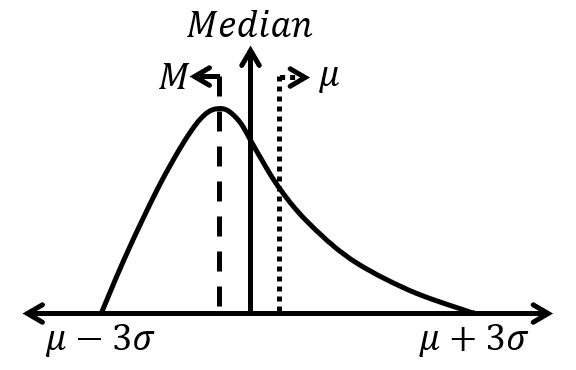
\includegraphics[width=0.3\textwidth]{figures/skewness.png}
    \caption{Gaussian normal distribution with skewness.}
    \label{fig:skewness}
\end{figure}

We design a vehicle speed model to reflect real-world vehicle speed scenarios and to evaluate the prediction accuracy for calculating the chunks that should be precached by predicting the dwell time within the coverage of the next RSU.
Within the area where the vehicles are located, their speeds follow an average speed, taking into account several factors such as rush hour congestion and hot spots.
Accordingly, we formulate the probability of the acceleration $a_{i}(t)$ of the vehicle $V_{i}$ at the time $t$ based on Gaussian distribution with skewness \cite{Azzalini} as follows:
\begin{equation}
    \begin{split}
        P[a=a_{i}(t)]=&\cfrac{2}{\omega\sqrt{2\pi}} e^{-\cfrac{(a-\xi)^{2}}{2\omega^{2}}} \\
                & \times\int_{-\infty}^{\alpha\left(\cfrac{a-\xi}{\omega}\right)} \cfrac{1}{\sqrt{2\pi}} e^{-\cfrac{q^2}{2}} dq,
    \end{split}
\end{equation}
where $\omega$ is the scale parameter, $\xi$ is the location parameter, and $\alpha$ is the shape parameter.
They are denoted as follows:
\begin{equation} 
    \xi = \mu-\omega\delta\sqrt{\cfrac{2}{\pi}}, \quad
    \omega = \cfrac{\sigma}{\sqrt{1-\cfrac{2\delta^{2}}{\pi}}}, \quad
    \alpha = \cfrac{\delta}{\sqrt{1-\delta^{2}}}, \end{equation}
where $\mu$ is the mean acceleration.
For the comfort of users in a vehicle, we assume that the range of the vehicle's acceleration is $[-5, 5] km/(h\times s)$, which means that the maximum acceleration $a_{max}$ is $5 km/(h\times s)$.
Therefore, $\mu$, which indicates the middle value of the range, is 0.
Then, $\delta$ is denoted as follows:
\begin{equation}
        |\delta| = \sqrt{\cfrac{\pi}{2} \cfrac{|\gamma|^{2/3}}{|\gamma|^{2/3}+(\cfrac{4-\pi}{2})^{2/3}}}.
\end{equation}
The sign of $\delta$ is the same as the sign of the skewness $\gamma$ that is denoted as follows:
\begin{equation}
        %\gamma = \cfrac{n}{(n-1)(n-2)} \sum^{n}_{x=1}\left( \cfrac{a_{x}(t)}{\sqrt{\cfrac{\sum^{n}_{x=1}(a_{x}(t))^{2}}{n}}} \right)^{-3},
        \gamma = \cfrac{n}{(n-1)(n-2)} \sum^{n}_{p=1}\left( \cfrac{\left(\sum^{n}_{q=1}(a_{(q)}(t))^{2} \right)^{1.5}}{a_{(p)}(t)^{3}n^{1.5}} \right),
\end{equation}
where $n$ is the number of samples.
We denotes the standard deviation $\sigma$ as follows:
\begin{equation}
    \sigma = \cfrac{a_{max}-\mu}{k},
\end{equation}
where $k$ is 2.576 in 99\% confidence interval.
Then, to make the acceleration follow the average speed within the area, we set the Mode value $M$ that is the shifted average value by skewness $\gamma$ as follows:
\begin{equation}
    \begin{split}
        M=&\xi+\omega m_o(\alpha) \\
         =& \begin{cases}
            - a_{max}\left( \cfrac{v_{cur}-v_{av}}{v_{max}-v_{av}}\right) & \text{if } v_{cur} > v_{av}, \\
            a_{max}\left( \cfrac{v_{cur}-v_{av}}{v_{min}-v_{av}}\right) & \text{if } v_{cur} \leq v_{av},
            \end{cases}
    \end{split}
\end{equation}
\begin{equation}
    m_o(\alpha) = \mu_{z} - \cfrac{\gamma\sqrt{1-\mu_{z}^{2}}}{2} - \cfrac{sgn(\alpha)}{2} e^{\left(-\cfrac{2\pi}{|\alpha|}\right)},
\end{equation}
where $\mu_{z}$ is $\delta(\sqrt{2/\pi})$ \cite{Azzalini}.


Based on the determined acceleration of $V_{i}$ according to $P[a = a_{i}(t)]$, we can denote the speed $v_{i}(t)$ of the vehicle $V_{i}$ after the time $t$ as follows:
\begin{equation}
    v_{i}(t) = v_{i}(0) + \sum_{q=0}^{t} a_{i}(q),
\end{equation}
where $v_{i}(0)$ is the current speed of $V_{i}$.
Through the velocity, we can calculate the distance $Dist_{i}(t)$ that the vehicle moves until the time $t$ as follows:
\begin{equation}
    Dist_{i}(t) = Dist_{i}(0) + \sum_{q=0}^{t} v_{i}(q),
\end{equation}
where $Dist_{i}(0)$ is the current location of the $V_{i}$.
With the integrated information between the distance traveled until time $t$ and the trajectory information from the navigator application, we can predict the location of the vehicle at the time $t$.

In the calculation, neither the current speed of $V_{i}$ nor the average speed of vehicles in the next RSU reflects the vehicle speed at the time when the precached chunks are downloaded in the next RSU.
Therefore, to reflect the road conditions of the next RSU in the calculation, the average speed over a period of time is taken into account, and the average speed can be obtained as follows:
\begin{equation}
    v_{av, j}(t) = \frac{\sum_{i\in Dwell_{j}}\sum_{q=0}^{t_{max}}v_{i, j}(t-q)}{Num(Dwell_{j})t_{max}},
\end{equation}
where $Dwell_{j}$ is the set of the vehicles that dwell within the coverage of $R_{j}$.
$Num(Dwell_{j})$ is the number of the vehicles in $Dwell_{j}$.
Therefore, we can use $v_{av, j}(t)$ to reflect conditions of the coverage area of $R_{j}$.


\subsection{Content Request Model}
To reflect a realistic environment in terms of vehicles' content requests, we design a content request model.
The total content set is $\mathbb{C}=\{C_{1}, \cdots, C_{C}\}$, where $C$ is the total number of the content set and $C_{c}$ denotes the $c$-th content.
Based on Zipf's law \cite{Zipf}, we define the popularity $Pop(C_{c})$ of each content $C_{c}$, where $Pop(C_{c})$ is the probability that $C_{c}$ is requested, and is calculated as follows:
\begin{equation}
    Pop(C_{c})=c^{-\alpha_{2}}\left(\sum^{C}_{k=1}k^{-\alpha_{2}}\right)^{-1},
\end{equation}
where $c$ indicates the popularity rank of $C_{c}$ and $\alpha_{2}$ is the Zipf exponent parameter.

Then, we define the probability that $C_{c}$ has its size $Size(C_{c})$ based on Gaussian distribution as follows:
\begin{equation}
    Pr_{size}[q=Size(C_{c})]=\cfrac{1}{\sigma_{3}\sqrt{2\pi}}e^{\cfrac{1}{2}\left( \cfrac{q-\mu_{3}}{\sigma_{3}}\right)^{2}},
\end{equation}
where $\sigma_{3}$ is the standard deviation and $\mu_{3}$ is the mean value.
To avoid the situation that the content size is smaller than 0, we set the standard deviation according to $\mu-3\sigma = 0$.

Also, we define the request frequency by designing the probability of the next request time $t_{req}$ by a vehicle $V_{i}$ based on the Poisson distribution as follows:
\begin{equation}
    Pr_{req}[t=t_{req}]=\lambda e^{-\lambda t},
\end{equation}
where $\lambda$ is the rate parameter, representing the average number of requests per unit of time.

Consequently, vehicles, considering content popularity, size, and request frequency distributions, individually decide their requested content at specified intervals.
This model enables a vehicle to request various content items while actively downloading another.
Furthermore, for fairness, content is randomly categorized as DSC or DTC.
In real-world scenarios, this model allows diverse content requests, ranging from real-time streaming services to background applications like software updates, enhancing the realism of the simulated environment.
    



\section{Content Storage Management and Precaching (CSMP) scheme} \label{sec.csmp}
In this section, we describe the details of our caching storage management and precaching scheme, taking into account the delay tolerance of the requested content.
We first present our CSM method based on an RSU's Caching Priority Table (CPT) for content requests by vehicles in the subsection \ref{subsec1}.
This table not only outlines the prioritization, but also includes a mode of the cached content.
Then, we describe our DSCP method in the subsection \ref{subsec2}.
In this scheme, we formulate the recalculation time using vehicle mobility based on a Gaussian distribution with skewness.
This recalculation time is critical to improving mobility prediction accuracy, which has a direct impact on QoS and user safety.
Finally, our DTCP method is provided in the subsection \ref{subsec3}, which makes use of cached RSUs while taking into account the tolerable delay of the requested content.
To optimize the utilization of backhaul link traffic, RSUs make informed decisions to select the most appropriate RSUs to participate in providing the requested DTC.
This optimization process is achieved through Integer Linear Programming (ILP) in our delay-tolerant content precaching method.



\subsection{Content Storage Management method} \label{subsec1}

\begin{figure*}[ht]
    \centering
    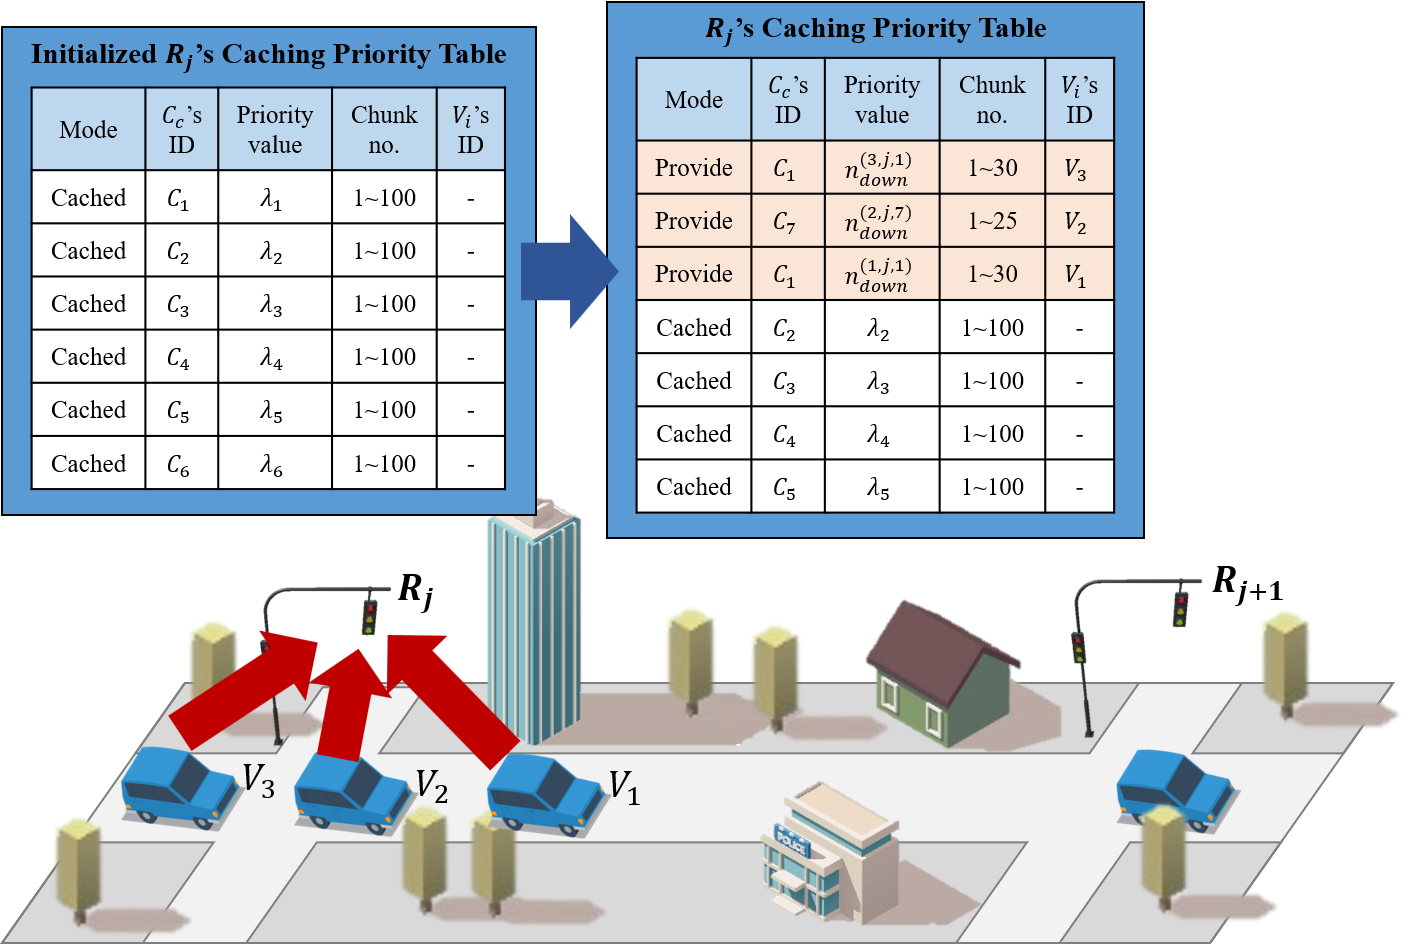
\includegraphics[width=0.9\textwidth]{figures/concept1.png}
    \caption{The Content Storage Management (CSM) method in the CSMP scheme: a change of $R_{j}$'s caching priority table in a situation where $R_{j}$ provides the requested contents to $V_{1}$, $V_{2}$, and $V_{3}$.}
    \label{fig:conc1}
\end{figure*}

We present our CSM method to ensure the prevention of inadvertently erasing cached contents.
For managing the content caching storage, we use the CPT in RSUs, which is to determine what content will be erased when the RSU's caching storage is fully filled.
Each entry in the CPT includes information about the requester vehicle ID, the requested content ID, priority mode, and priority value.
Our proposed method involves the classification of cached contents by the CPT based on different priority modes, each assigned a priority value according to its mode.
The method consists of three modes:
\begin{itemize}
    \item $Provide$ mode: 
    The content in this mode is actively provided within the RSU's coverage.
    To maintain fairness, the requested content by a requester vehicle, which has already received a significant number of chunks, is assigned low priority.
    Consequently, the priority value for this mode is denoted by the number of the received chunks.
    
    \item $Precached$ mode:
    The content in this mode is precached at the current RSU based on the mobility information of the requester vehicle by the calculation of the previous RSU.
    To avoid access delays associated with content retrieval, the priority value for this mode is defined as the remaining time to provision, which is specifically the time until the requester vehicle enters the current RSU's coverage.
    
    \item $Cached$ mode:
    The content in this mode is initially cached based on its popularity or has completed the provisioning process.
    Since the content is not expected to be requested in the immediate future, the priority value takes into account the probability of being requested.
    Therefore, the priority value of this mode is determined by the popularity of the content.
\end{itemize}
This comprehensive classification and prioritization strategy ensures efficient content management within the RSU's storage, minimizing the impact of content elimination on content availability and user experience.

An RSU's storage can be empty for various reasons such as installing a new RSU or resetting the RSU.
In such situations, the caching storage (CS) is precached with popular content that vehicles are likely to request, as shown in the initialized CPT in Figure \ref{fig:conc1}.
Then, their mode is labeled as $Cached$ because they are not cached due to a request and are not immediately delivered to the vehicle.
Also, since the likelihood of cached contents being requested by vehicles is related to their popularity, we set their priority values and rank them by popularity based on Zipf's law.

When a vehicle requests content from an RSU, the RSU first looks for the requested content in its caching storage.
If the content is found in the RSU's caching storage, the RSU changes the content's $Cached$ mode to $Provide$ mode and puts the downloaded size by the vehicle in its CPT, as shown in $V_{1}$ in Figure \ref{fig:conc1}.
Otherwise, the RSU takes the requested content from the content server or another cached RSU via backhaul links based on CCN policy.
Then, the taken content's mode becomes $Provide$ mode, as shown in $V_{2}$ in Figure  \ref{fig:conc1}.
However, in that case, if RSU's caching storage was already full, the RSU erases the lowest priority $Cached$ mode or $Precached$ mode content in its CPT and caching storage.
In Figure \ref{fig:conc1}, $C_{6}$ is erased to cache taken $C_{7}$ because the CS of $R_{j}$ is full.
Unexpectedly, when the $Provide$ mode content is re-requested by another requester vehicle, the RSU adds a re-requests entry containing the requester vehicle ID in its CPT.
Therefore, the CPT of the RSU has entries that have the duplicated content ID but a different requester vehicle ID, as shown in $V_{3}$ in Figure \ref{fig:conc1}.
To ensure fairness, if the caching storage is fully filled with contents from the $Provide$ mode, the RSU will stop providing the content that has the largest downloaded size to give a chance to the requester vehicle that starts downloading content.
Thus, a priority value in this mode is the received content size $n^{i,j,c}_{down}$ that $C_{c}$ has already been provided by $V_{i}$ from $R_{j}$, as shown in Figure \ref{fig:conc1}.
In order to resume downloading the content after other vehicles receive more chunks of their requested content and the priority of that content has been lowered, the RSU erases the content with the lowest priority value from the CS but not from the CPT, and stops providing the content.
Therefore, the RSU will resume downloading the stopped content when the priority values in other entries become lower.


\subsection{Delay Sensitive Content Precaching method} \label{subsec2}

\begin{figure*}[ht]
    \centering
    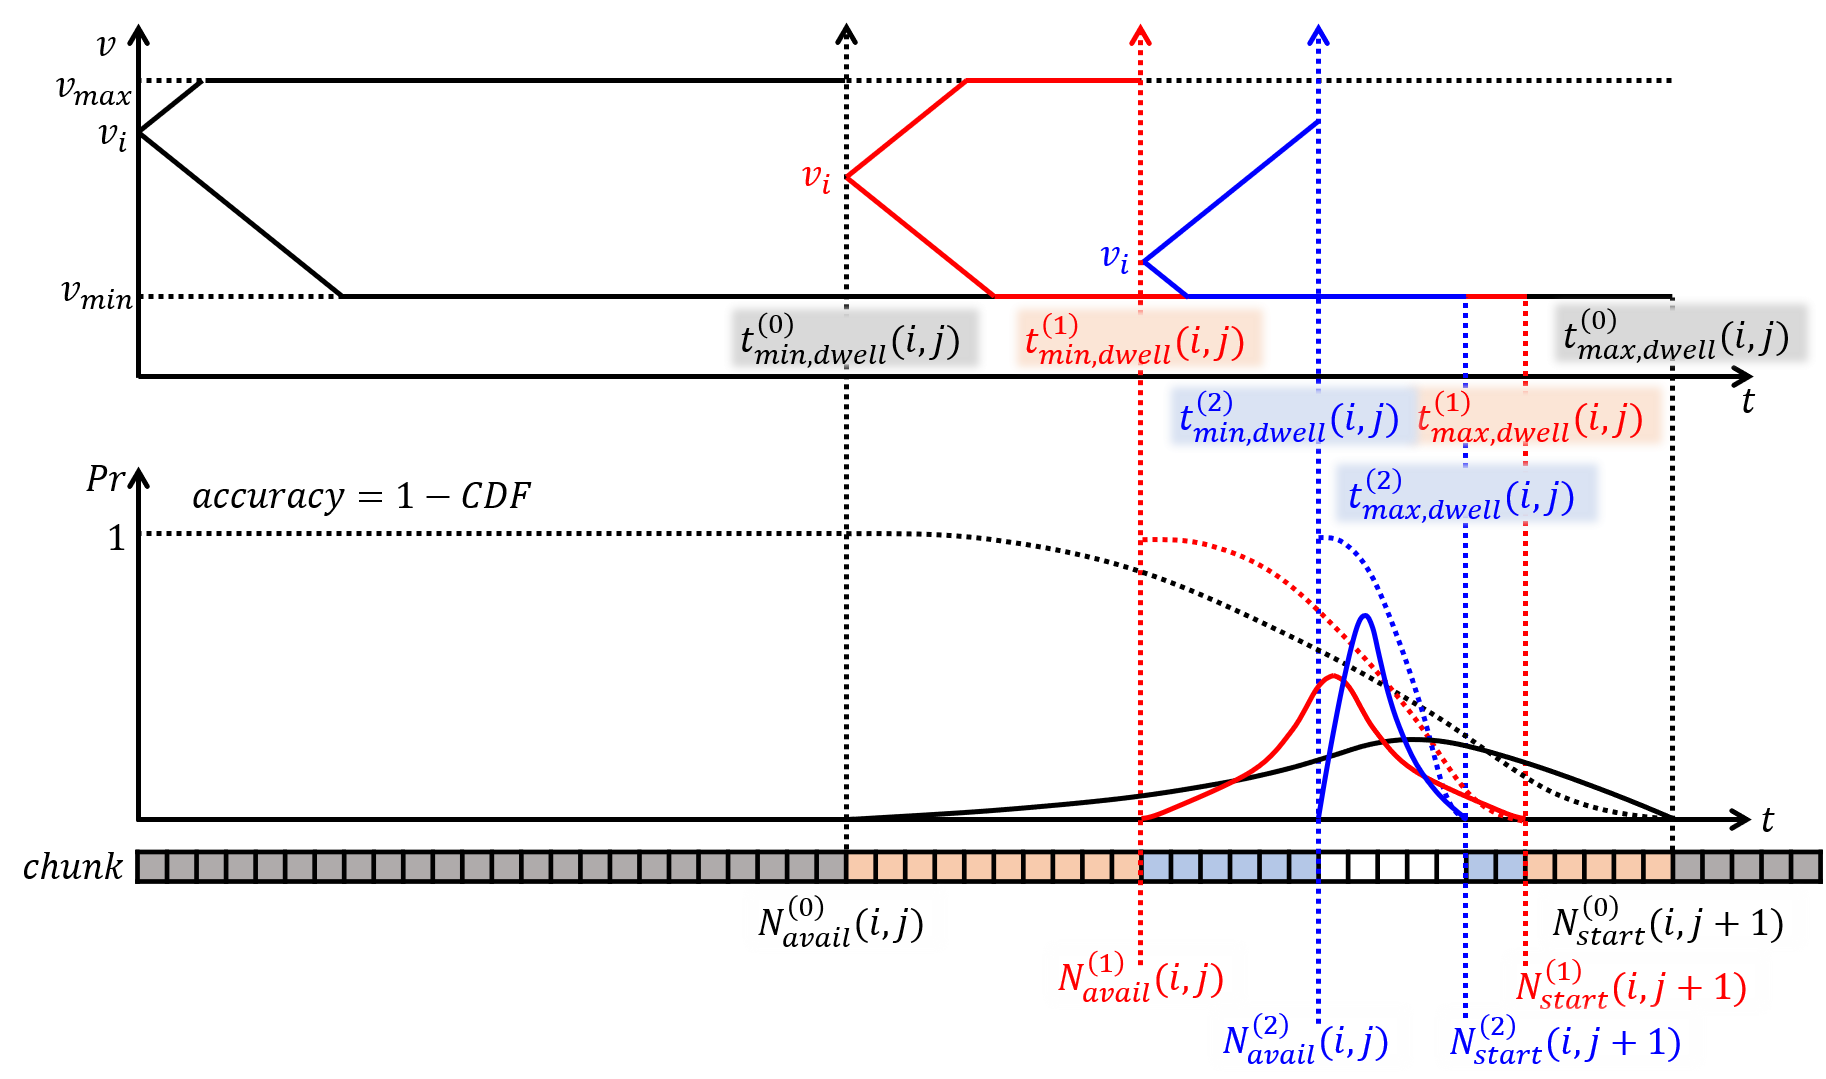
\includegraphics[width=0.9\textwidth]{figures/tgap.png}
    \caption{A concept of $t^{(m)}_{gap}$, where the initial calculation process in black line graphs, the first recalculation process in red line graphs, and the second recalculation process in blue line graphs.}
    \label{fig:tgap}
\end{figure*}

We design the Delay Sensitive Content Precaching (DSCP) method to ensure the delay minimization for DSC download in this subsection.
For a content request by a vehicle, an RSU employs predictive analytics to estimate the dwell time of the vehicle, which plays a crucial role in determining the necessity of precaching.
If the predicted dwell time is short or the requested content is substantial in size, the RSU may be unable to complete the delivery of all chunks of the content within its coverage.
In such cases, the responsibility falls to the next RSU the vehicle will encounter later, which must precache the remaining chunks to minimize access delays.
However, this way presents a dilemma: if the next RSU precaches a large number of chunks, it will consume additional backhaul link traffic and risk exceeding its storage capacity, potentially resulting in the inadvertent erase of other critical content.
Conversely, precaching too few chunks can result in insufficient content for delivery within the RSU's coverage, leading to increased access delays to get the rest of the chunks.

Therefore, the challenge for efficient content precaching is to accurately predict the optimal number of chunks to precache, taking into account factors such as backhaul link traffic, storage efficiency, and access delays.
To achieve this challenge, RSUs should rely on accurate dwell time predictions for calculating the optimal number of chunks.
Since the mobility of vehicles is usually constrained by road structures, legal speed limits, and interactions among vehicles, a vehicle's speed becomes an indicator of the average speed at its current location.
Consequently, RSUs manage and utilize the average speed information within their coverage areas for conducting effective mobility prediction.

When a vehicle $V_{i}$ requests delay-sensitive content $C_{c}$ from an RSU $R_{j}$, the RSU calculates the minimum dwell time $t^{(0)}_{min, dwell}(i,j)$ required to secure the guaranteed number of chunks for $C_{c}$ for $V_{i}$ as follows:
\begin{equation}
    v^{(0)}_{max, i}(t)=\begin{cases}
        v_{i}+a_{max}t & \text{if } v_{i}+a_{max}t < v_{max}\\
        v_{max} & \text{else},
    \end{cases}
\end{equation}
\begin{equation}
    D_{j}-x^{(0)}_{ij}=\int^{t^{(0)}_{min, dwell}(i,j)}_{0} v^{(0)}_{max, i}(t) dt,
\end{equation}
where $v^{(0)}_{max, i}(t)$ is the maximum speed that $V_{i}$ can have at the time $t$ and $(0)$ means this calculation is not repeated for mobility prediction.
$a_{max}$ represents the maximum acceleration for user comfort, while $v_{max}$ represents the legal maximum speed limit of the road on which $V_{i}$ moves.
$D_{j}$ represents the communication range of $R_{j}$, and $x^{(0)}_{ij}$ represents the distance that $V_{i}$ has moved within $R_{j}$'s coverage up until now.
Therefore, $D_{j}-x^{(0)}_{ij}$ indicates the remaining distance until $V_{i}$ leaves the communication range of $R_{j}$.

Using $t^{(0)}_{min, dwell}(i,j)$, we calculate the number of available chunks $N^{(0)}_{avail}(i,j)$ as follows: % and if $R_{j}$ does not have enough chunks, it will begin precaching for $C_{c}$.
\begin{equation}
    N^{(0)}_{avail}(i,j)=\cfrac{t^{(0)}_{min, dwell}(i,j)\times r_{j, av}(t)}
    {s},
\end{equation}
where $r_{j, av}(t)$ represents the average transmission rate of $R_{j}$ and $s$ represents the size of one chunk.
If $R_{j}$ does not have the chunks, it retrieves them from other RSUs or the content server.
$R_{j}$ designates the chunks as being in $Provid$ mode and sets their priority value.
However, if $N^{(0)}_{avail}(i,j)$ is less than the total number of chunks, $R_{j}$ calculates the maximum dwell time $t^{(0)}_{max, dwell}(i,j)$ to determine which chunks the next RSU $R_{j+1}$ should precache as follows:
\begin{equation}
    v^{(0)}_{min, i, j}(t)=\begin{cases}
        v_{i}-a_{max}t & \text{if } v_{i}-a_{max}t > v_{min, j}\\
        v_{min, j} & \text{else},
    \end{cases}
\end{equation}
\begin{equation}
    D_{j}-x^{(0)}_{ij}=\int^{t^{(0)}_{max, dwell}(i,j)}_{0} v^{(0)}_{min, i, j}(t) dt,
\end{equation}
where $v^{(0)}_{min, i, j}(t)$ represents the minimum speed that $V_{i}$ can have at the time $t$ based on $a_{max}$.
$v_{min, j}$ is the minimum speed that vehicles can have in the communication coverage of $R_{j}$.
$R_{j}$ updates $v_{min, j}$ based on the maximum dwell time of vehicles within $R_{j}$'s coverage to reflect a realistic scenario and prevent the situations where $t^{(0)}_{max, dwell}(i,j)=\infty$ and $v^{(0)}_{min, i, j}=0$.
Then, the first chunk number $N^{(0)}_{start}(i,j+1)$ that $R_{j+1}$ should precache can be formulated as follows:
\begin{equation}
    N^{(0)}_{start}(i,j+1) = \cfrac{t^{(0)}_{max, dwell}\times r_{j+1, av}(t)}
    {s}.
\end{equation}
Additionally, we can formulate the final chunk number $N^{(0)}_{end}(i, j+1)$ that $R_{j+1}$ can guarantee to provide to $V_i$ through precaching by using the following equations (22) and (23):
\begin{equation}
    v^{(0)}_{max, i, j+1}(t)=\begin{cases}
        v_{av, j}-a_{max}t & \text{if } v_{av, j}-a_{max}t > v_{max}\\
        v_{max} & \text{else},
    \end{cases}
\end{equation}
\begin{equation}
    D_{j+1}=\int^{t^{(0)}_{min, dwell}(i,j+1)}_{t^{(0)}_{max, dwell}(i,j)} v^{(0)}_{min, i, j+1}(t-t^{(0)}_{max, dwell}(i,j)) dt,
\end{equation}
\begin{equation}
    N^{(0)}_{end}(i, j+1)=\cfrac{t^{(0)}_{min, dwell}(i,j+1)\times r_{j+1, av}(t)}{s}.
\end{equation}


If $N^{(0)}_{start}(i,j+1)$ is less than the total number of chunks for $C_{c}$, $R_{j}$ will not send a $Precache$ packet to $R_{j+1}$ to request precaching.
The $Precache$ packet is intended to allow $R_{j+1}$ to precache the chunks of $C_{c}$.
Since $C_{c}$ has a limited chunk number, $N^{(0)}_{end}(i, j+1)$ becomes the last chunk number of $C_{c}$ when it is bigger than the total number of $C_{c}$'s chunks.
The $Precache$ packet includes $t^{(0)}_{max, dwell}(i,j)$, the ID of $V_{i}$, the ID of $C_{c}$, $N^{(0)}_{start}(i,j+1)$, and $N^{(0)}_{end}(i, j+1)$.
When $R_{j+1}$ receives the $Precache$ packet, it precaches the chunks of $C_{c}$ that range between $N^{(0)}_{start}(i,j+1)$ and $N^{(0)}_{end}(i, j+1)$, as shown in Figure \ref{fig:conc2}.
Then, it adds the precached chunks as a $Precached$ mode in its CPT and sets their priority value to $t^{(0)}_{max, dwell}(i,j)$ in order to prevent erasing content that will soon be requested, because $t^{(0)}_{max, dwell}(i,j)$ denotes the expected time to arrive at the next RSU.
That is, a vehicle with a smaller $t^{(0)}_{max, dwell}(i,j)$ will enter the coverage area of the next RSU faster and request the precached content.


\begin{figure*}
    \centering
    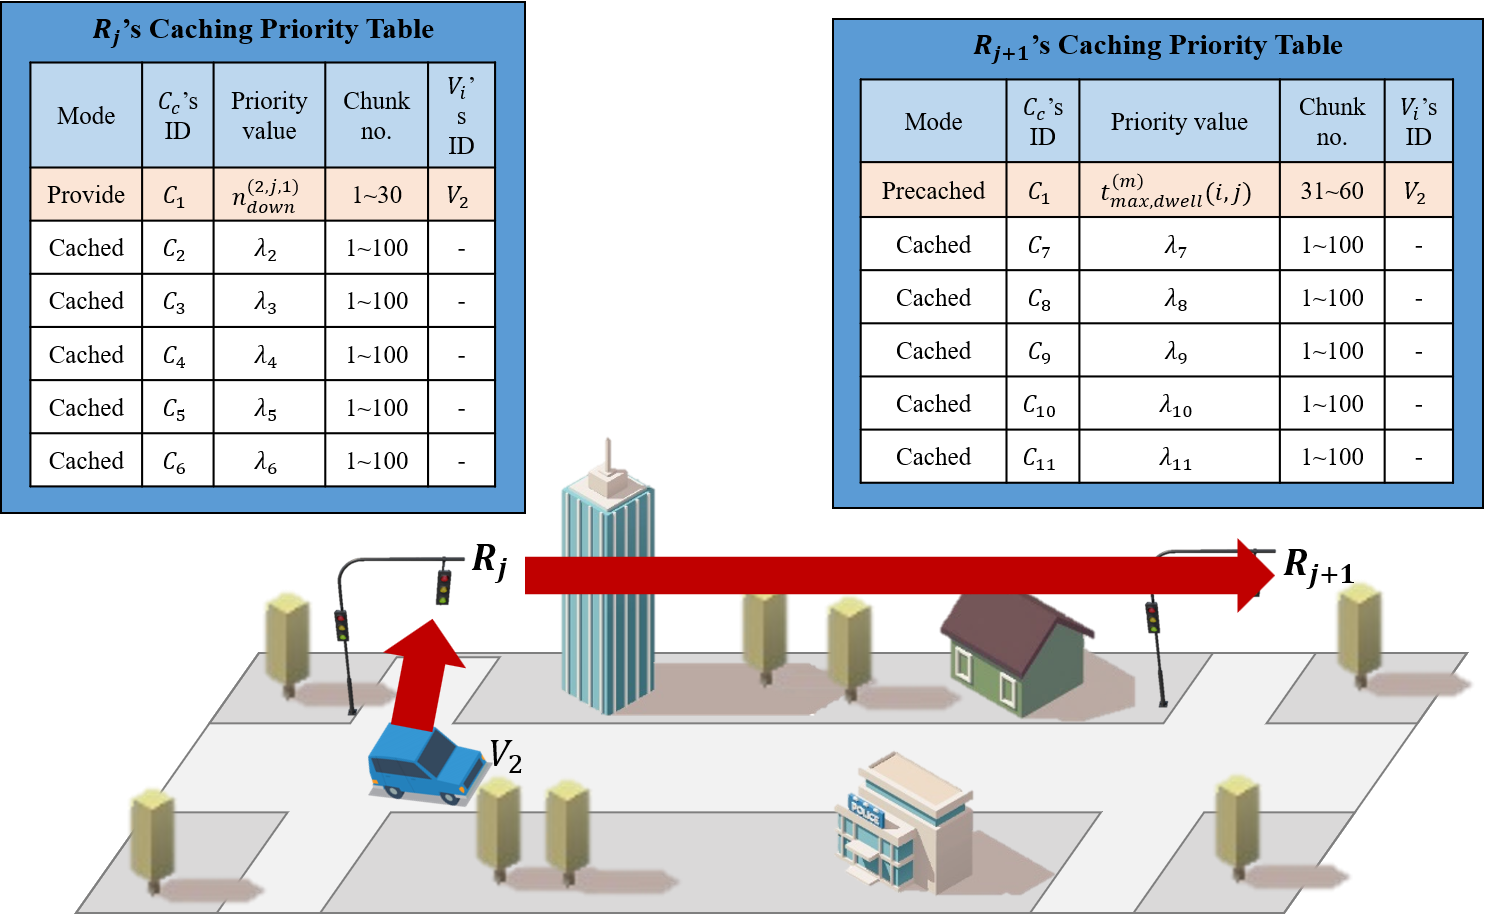
\includegraphics[width=0.9\textwidth]{figures/concept2.png}
    \caption{The Delay-Sensitive Content Precaching (DSCP) method: CPT of $R_{j+1}$ in a situation where $R_{j}$ lets $R_{j+1}$ to precache $C_{1}$ for $V_{2}$.}
    \label{fig:conc2}
\end{figure*}


$R_{j}$ prepares the chunks according to expected $N^{(0)}_{avail}(i,j)$ that is based on the minimum dwell time $t^{(0)}_{min, dwell}(i,j)$ and $R_{j+1}$ precaches the chunks according to expected $N^{(0)}_{start}(i,j+1)$ that is based on the maximum dwell time $t^{(0)}_{max, dwell}(i,j)$.
Therefore, a temporal gap $t^{(0)}{gap}$ emerges between $N^{(0)}_{avail}(i,j)$ and $N^{(0)}_{start}(i,j+1)$ due to the inherent uncertainty in the mobility prediction.
To improve the prediction accuracy, $R{j}$ recalculates $N^{(0)}_{avail}(i,j)$ and $N^{(0)}_{start}(i,j+1)$ after $t^{(0)}_{min, dwell}(i,j)$ because $t^{(0)}_{min, dwell}(i,j)$ indicates that the vehicle must leave at this time and its accuracy is 100\% until the time.
Thus, the recalculated values are $t^{(1)}_{max, dwell}(i,j)$, $t^{(1)}_{min, dwell}(i,j)$, $N^{(1)}_{avail}(i,j)$ and $N^{(1)}_{start}(i,j+1)$.
Whenever the recalculation is repeated, the iterator increases by 1.
$R_{j}$ prepares additional cached chunks as $Provide$ mode based on $N^{(1)}_{avail}(i,j)$, and sends a $Precache$ packet, which includes $t^{(1)}_{max, dwell}(i,j)$ and $N^{(1)}_{start}(i,j+1)$.
Meanwhile, $R_{j+1}$ conducts precaching of additional chunks based on $N^{(1)}_{start}(i,j+1)$ as $Precached$ mode, and updates their priority value to $t^{(1)}_{max, dwell}(i,j)$.

At each $m$-th recalculation time $t^{(m)}_{min, dwell}(i,j)$, $R_{j}$ iteratively calculates $t^{(m)}_{max, dwell}(i,j)$, $N^{(m)}_{avail}(i,j)$ and $N^{(m)}_{start}(i,j+1)$.
The gap, which is expressed as $t^{(m)}_{gap} = t^{(m)}_{min, dwell}(i,j) - t^{(m)}_{max, dwell}(i,j)$, is reduced because there is not enough time to change the speed of $V_i$ due to the reduced distance.
Therefore, the recalculations of $R_{j}$ continue until the prediction accuracy reaches 99\%, which is denotes by $1-(t^{(m)}_{gap}/t^{(m)}_{max, dwell}(i,j))=0.99$, because the difference between $t^{(m)}_{min, dwell}(i,j)$ and $t^{(m)}_{max, dwell}(i,j)$ is almost the same.

As shown in Figure \ref{fig:tgap}, the iterative recalculation process continues until the prediction accuracy reaches 99\%.
The above graphs represent the time-velocity relationships, while the below graphs show the time-probability relationships.
The solid line graphs among the below graphs represent the probability distribution of $V_{i}$'s location based on a Gaussian distribution with skewness, while the dashed line graphs represent the accuracy of the dwell time prediction.
This accuracy can be calculated using $1-CDF$, where $CDF$ represents the cumulative distribution function of $V_{i}$'s location probability.
By utilizing variables such as $v_{i}$, $v_{max}$, $v_{min}$, and $a_{max}$, $R_{j}$ can accurately calculate $t^{(0)}_{max, dwell}(i,j+1)$ and $t^{(0)}_{min, dwell}(i,j+1)$ with a 100\% accuracy.
As the provisioning and precaching chunks are recalculated, the gap $t^{(m)}_{gap}$ between predicted and actual dwell times decreases, indicating an increasing accuracy of the predictive model.

Once $V_{i}$ departs from $R_{j}$, all content pertaining to $V_{i}$ in $R_{j}$'s CPT is transitioned to the $Cached$ mode, and $R_{j}$ erases $V_{i}$'s information.
Then, after moving its traveling route, $V_{i}$ enters the communication coverage of $R_{j+1}$.
Upon recognizing the arrival of $V_{i}$ through its requests, $R_{j+1}$ updates the entries of all contents related to $V_{i}$ to $Provide$ mode in its CPT, and assigns respective priority values to them.
Therefore, the DSC, which depends significantly on prediction accuracy, can be precached with high accuracy to minimize delays caused by recalculation.



\subsection{Delay Tolerant Content Precaching method} \label{subsec3}
Our DTCP method provides efficient precaching for DTC because a vehicle can request DTC according to its content characteristics of content services and applications.
Especially, to optimize the consumption of backhaul link traffic, we can use cached RSUs (i.e., RSUs that store the requested DTC) deployed along the path of a requester vehicle to provide DTC, which can withstand delays to up to its tolerable limit.
When a vehicle $V_{i}$ requests content $C_{c}$ to an RSU $R_{j}$, if the content is DTC, $R_{j}$ estimates the delay tolerance of $C_{c}$ based on its tolerable delay $t_{tol, i, c}$, the number of remaining chunks $N_{remain, i, c}$, and the dwell time $t_{dwell}(i,j)$.
Therefore, $R_{j}$ calculates the dwell time $t_{dwell}(i,j)$ of $V_{i}$ to determine whether it has enough time to withstand delay as follows:
\begin{equation}
    t_{dwell}(i,j)=\cfrac{D_{j}-x_{ij}}{v_{av,j}},
\end{equation}
where $x_{ij}$ represents the distance that $V_{i}$ has moved within the communication coverage of $R_{j}$ up to the present moment.
If $t_{tol, i, c}$ is less than $t_{dwell}(i,j) + t_{dwell}(i,j+1)$, $R_{j}$ classifies $C_{c}$ for $V_{i}$ as a DSC because it does not have enough cached RSUs within $t_{tol, i, c}$, where $x_{i(j+1)}$ is 0 because $V_{i}$ is not yet in $R_{j+1}$.
Additionally, $C_{c}$ for $V_{i}$ is classified as a DSC if $V_{i}$ lacks sufficient time to tolerate delays in receiving the remaining chunks of $C_{c}$.
$R_{j}$ calculates the remaining time $t_{remain, i, c}$ that $V_{i}$ needs to receive the remaining chunks as follows:
\begin{equation}
    t_{remain, i, c} = \sum^{N_{remain, i, c}}_{n=1} \cfrac{s}{r_{j, av}}.
\end{equation}
When $t_{remain, i, c}$ is less than $t_{tol, i, c}$, $R_{j}$ uses an error handling mechanism to address prediction inaccuracies.
This mechanism takes into account the available time $t_{dwell}(i,j+1)$ for utilization by a single RSU.
If $t_{tol, i, c}$ is less than $t_{remain, i, c} + t_{dwell}(i,j+1)$, $R_{j}$ identifies $C_{c}$ as a DSC.
This is because there is not enough time to deliver $C_{c}$ to $V_{i}$ within $t_{tol, i, c}$, even when considering the error handling time.
Otherwise, $C_{c}$ is handled as a DTC for precaching.

To determine if there are sufficient cached RSUs to provide $C_{c}$ to $V_{i}$ within $t_{tol, i, c}$, $R_{j}$ sends a $Travel$ packet to the last RSU $R_{j+M}$ that $V_{i}$ can reach within $t_{tol, i, c}$, where $M$ represents the number of RSUs that can be encountered by $V_{i}$ within $t_{tol, i, c}$.
$R_{j}$ sends the packet to the next RSU $R_{j+1}$ based on the trajectory of $V_{i}$.
On receiving the packet, $R_{j+1}$ also sends it to its next RSU $R_{j+2}$. 
This process continues that the packet is eventually forwarded to the last RSU $R_{j+M}$ based on $V_{i}$'s trajectory


Then, the $Travel$ packet contains $t_{tol,i,c}$, $V_{i}$'s trajectory and ID, expected travel time $E[t_{travel,i}]$, and $N_{avail, i, c}(j)$, where $E[t_{travel,i}]$ is initialized as $t_{dwell,i,j}$, as shown in Figure \ref{fig:conc3}.
When the $m$-th next RSU $R_{j+m}$ receives the packet, it adds its $t_{dwell, i, (j+m)}$ to $E[t_{travel,i}]$, and compares the updated $E[t_{travel,i}]$ with $t_{tol,i,c}$ to determine whether it is the last RSU $R_{j+M}$.
If $E[t_{travel,i}]$ is less than $t_{tol,i,c}$, it indicates that $R_{j+m}$ is not equal to $R_{j+M}$.
Thus, $R_{j+m}$ adds its ID, $N_{avail, i, c}(j+m)$, and caching state $s_{j+m, c}$ to the packet and forwards the updated packet to the next RSU according to $V_{i}$'s trajectory that is included in the packet, where $s_{j+m, c}$ represents the caching state set of $C_{c}$'s chunks and is denoted as $s_{j+m, c}=\{s_{j+m}(h_{c,1}), \cdots, s_{j+m}(h_{c, N_{c}})\}$, as shown in Figure \ref{fig:conc3}.
If $R_{j+m}$ has $n$-th chunk of $C_{c}$, $s_{j+m}(h_{c,n})$ is 1.
If $R_{j+m}$ doesn't, $s_{j+m}(h_{c,n})$ is 0, denoted as $s_{j+m}(h_{c,n})=\{0,1\}$.
However, if $E[t_{travel,i}]$ becomes bigger than $t_{tol,i,c}$, it means $R_{j+m}$ is the last RSU $R_{j+M}$.
Based on the information contained in the packet, $R_{j+M}$ selects the cached RSUs to provide $C_{c}$ to $V_{i}$ without using a precaching process that consumes additional backhaul link traffic.
This is because $C_{c}$, which is a DTC, does not require immediate provision.
To optimize the number of provided chunks, $R_{j+M}$ optimally selects the cached RSUs using an ILP approach as follows:
\begin{equation}
    max \sum^{N_{c}}_{n=N_{avail,i,c}(j)}\sum^{M}_{m=1}s_{j+m}(h_{c,n})\times\xi_{cached}(j+m,h_{c,n})\times(1+\omega_{m,c})
\end{equation}
\begin{equation} \label{eq:const1}
    s.t. \sum^{N_{c}}_{n=N_{avail,i,c}(j)}\xi_{cached}(j+m,h_{c,n})\leq N_{avail,i,c}(j+m)
\end{equation}
\begin{equation} \label{eq:const2}
    \sum^{M}_{m=1}\xi_{cached}(j+m,h_{c,n})\leq 1
\end{equation}
\begin{equation} \label{eq:const3}
    \xi_{cached}(j+m,h_{c,n})\leq s_{j+m}(h_{c,n})
\end{equation}
\begin{equation} \label{eq:const4}
    s_{j+m}(h_{c,n})=\{0,1\}
\end{equation}
\begin{equation} \label{eq:const5}
    \xi_{cached}(j+m,h_{c,n})=\{0,1\}
\end{equation}
where $\xi_{cached}(j+m,h_{c,n})$ is the value for the optimal selection.
Therefore, if $R_{j+m}$ prepares $n$-th chunk of $C_{c}$, $\xi_{cached}(j+m,h_{c,n})$ is 1.
Otherwise, it is 0.
Equation (\ref{eq:const1}) restricts the number of preparation chunks to the number of available chunks for each RSU $R_{j+m}$, because the RSU has limited time to provide the chunks.
Equation (\ref{eq:const2}) ensures that other RSUs do not precache $h_{c,n}$, which has already been assigned to be provided by $R_{j+m}$.
Equation (\ref{eq:const3}) means that $R_{j+m}$ cannot be ready for providing $h_{c,n}$ if it does not store $h_{c,n}$ in its caching storage.
The equation (\ref{eq:const4}) and the equation (\ref{eq:const5}) denote the characteristics of $s_{j+m}(h_{c,n})$ and $\xi_{cached}(j+m,h_{c,n})$, respectively.
The weight value $\omega_{m,c}$ is used to select an RSU when multiple RSUs have $h_{c,n}$ in their caching storage.
To avoid making $\omega_{m,c}$ the primary consideration, the sum of all $\omega_{m,c}$ must be less than 1.
This is because the primary variable $\xi_{cached}(j+m,h_{c,n})$ can be 1.
For this reason, we denote $\omega_{m,c}$ as follows:
\begin{equation}
    \omega_{m,c} = \cfrac{m}{N_{c}\times M}.
\end{equation}
Based on $\omega_{m,c}$, the RSU closest to $V_{i}$ is more likely to be selected to reduce caching burden and delays.
To determine whether the cached RSUs are sufficient to provide all of the chunks of $C_{c}$, $R_{j+M}$ compares $N_{c}$ to the total number of selected chunks $N_{cached, i, c}$, denoted as follows:
\begin{equation}
    N_{cached, i, c} = \sum^{N_{c}}_{n=N_{avail,i,c}(j)}\sum^{M}_{m=1}\xi_{cached}(j+m,h_{c,n}).
\end{equation}


\begin{figure*}
    \centering
    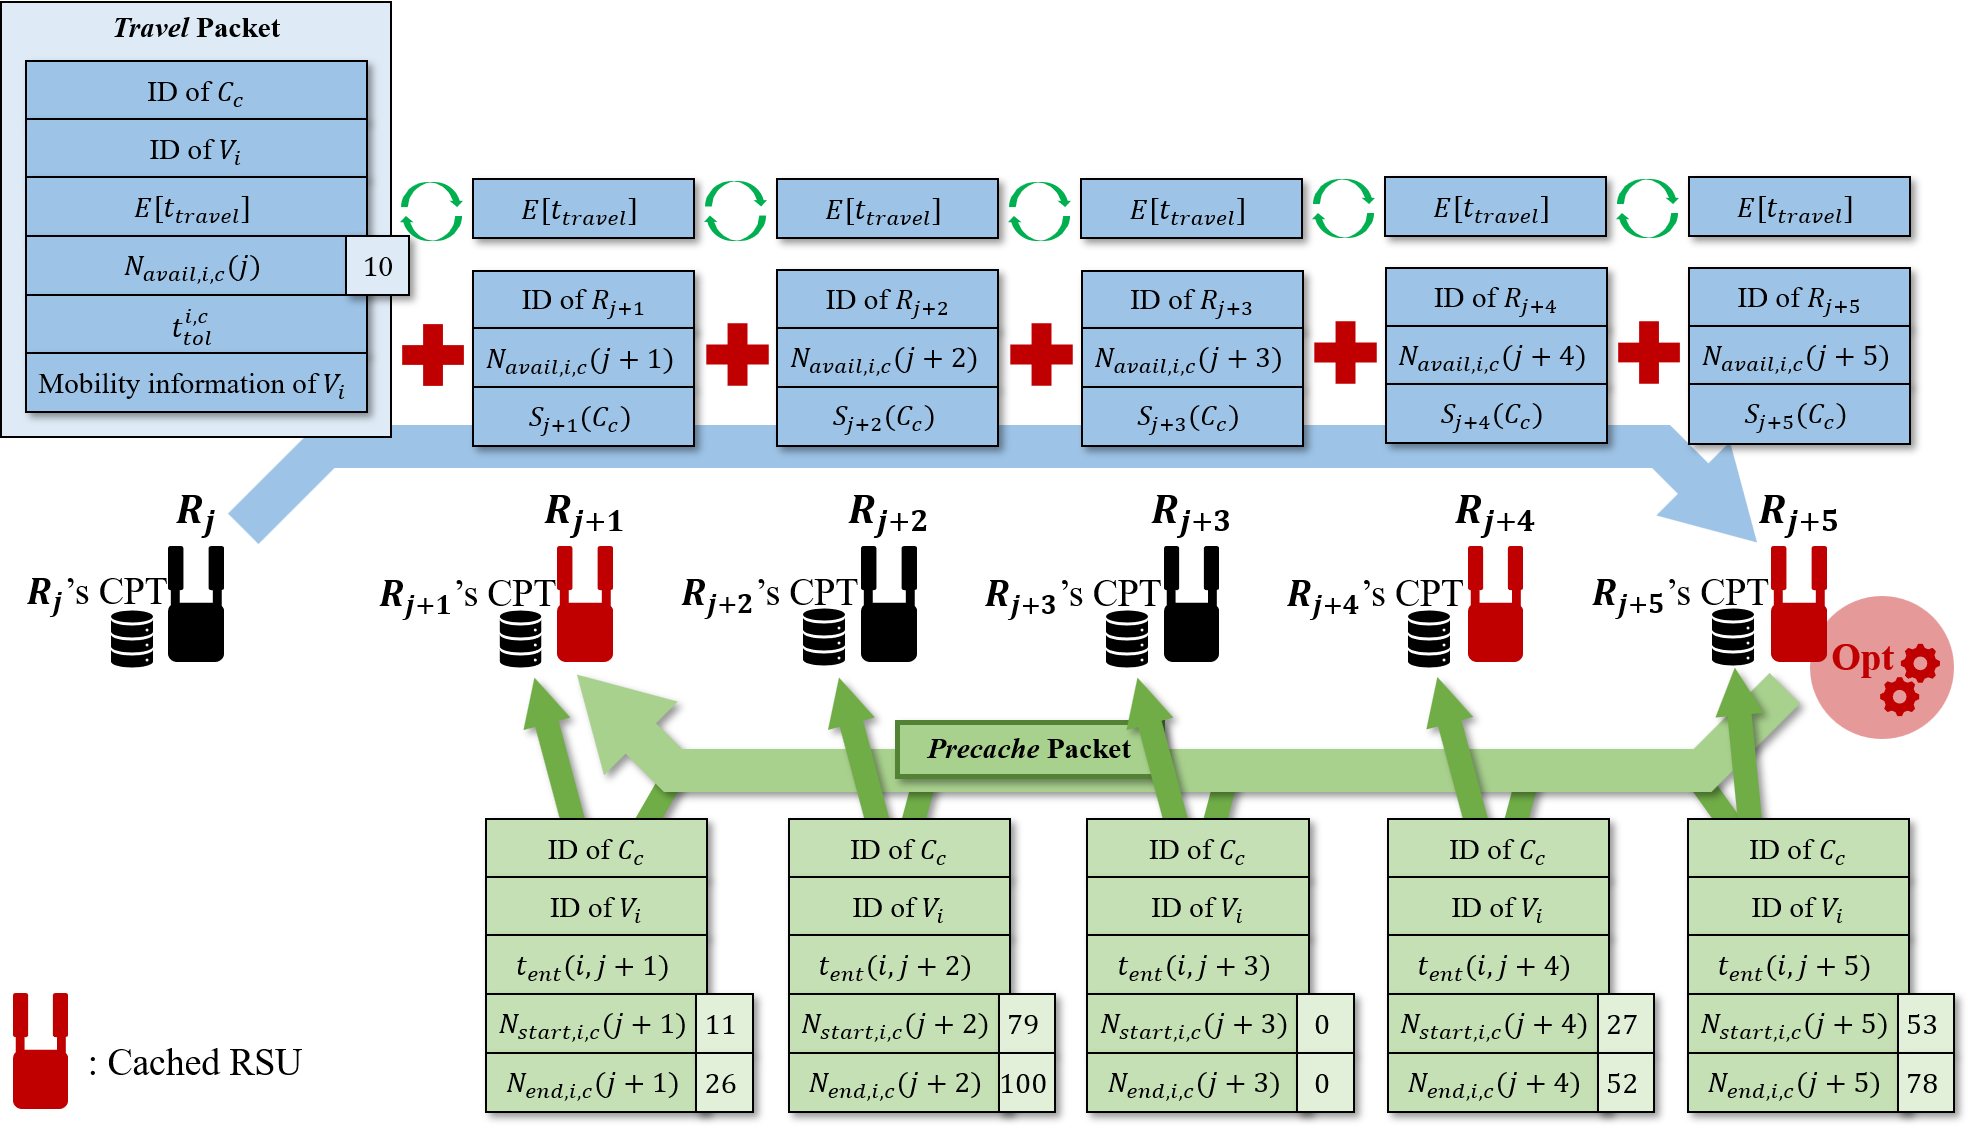
\includegraphics[width=\textwidth]{figures/conc3.png}
    \caption{The Delay-Tolerant Content Precaching (DTCP) method: The forwarded $Travel$ packet and $Precached$ packet when the requested DTC consists of 100 chunks and $K$ is 5.}
    \label{fig:conc3}
\end{figure*}

If $N_{cached, i, c}$ is greater than $N_{c}$, it indicates that there are sufficient cached RSUs to provide $C_{c}$ to $V_{i}$ within $t_{tol,i,c}$ without any additional backhaul link traffic.
However, if $N_{c}$ is greater than $N_{cached, i, c}$, it indicates that the number of the cached RSUs within $t_{tol,i,c}$ is insufficient.
Therefore, in that case, $R_{j+M}$ must select other RSUs to precache $C_{c}$.
Prior to making the selection, $R_{j+M}$ calculates the number of remaining chunks using $N_{remain,i,c}=N_{c}-N_{cached,i,c}$.
Then, $R_{j+M}$ optimally chooses additional RSUs using an ILP approach as follows:
\begin{equation}
    max \sum^{N_{c}}_{n=N_{avail,i,c}(j)}\sum^{M}_{m=1}(1-s_{j+m}(h_{c,n}))\times\xi_{prec}(j+m,h_{c,n})\times(1+\omega_{m,c})
\end{equation}
\begin{equation}
    s.t. \sum^{N_{c}}_{n=N_{avail,i,c}(j)}\xi_{prec}(j+m,h_{c,n})\leq N_{avail,i,c}(j+m)
\end{equation}
\begin{equation}
    \sum^{M}_{m=1}\xi_{prec}(j+m,h_{c,n})\leq 1
\end{equation}
\begin{equation}
    \xi_{prec}(j+m,h_{c,n})\leq1-s_{j+m}(h_{c,n})
\end{equation}
\begin{equation}
    s_{j+m}(h_{c,n})=\{0,1\}
\end{equation}
\begin{equation}
    \xi_{cached}(j+m,h_{c,n})=\{0,1\}
\end{equation}
where $\xi_{prec}(j+m,h_{c,n})$ is the value for letting $R_{j+m}$ to precache the chunk $h_{c,n}$ when it is 1.
If $R_{j+m}$ does not provide $h_{c,n}$ to $V_{i}$, $\xi_{prec}(j+m,h_{c,n})$ is 0.
After the optimization, the last RSU $R_{j+M}$ makes a $Precache$ packet containing $\xi_{cached}(j+m,h_{c,n})$, $\xi_{prec}(j+m,h_{c,n})$, $V_{i}$'s ID, and trajectory, as shown in Figure \ref{fig:conc3}.
The packet is then forwarded from $R_{j+M}$ to its previous RSU $R_{j+M-1}$ based on the trajectory of $V_{i}$.
Based on the forwarded order in the $Travel$ packet, the $Precache$ packet is forwarded in reverse up to $R_{j+1}$.
Upon receiving the $Precache$ packet, $R_{j+m}$ verifies $\xi_{cached}(j+m,h_{c,n})$ and $\xi_{prec}(j+m,h_{c,n})$ in the packet.
$\xi_{cached}(j+m,h_{c,n})$ and $\xi_{prec}(j+m,h_{c,n})$ can each have a value of either 0 or 1.
If $\xi_{cached}(j+m,h_{c,n})$ is 1, then $\xi_{prec}(j+m,h_{c,n})$ must be 0.
If $\xi_{cached}(j+m,h_{c,n})$ is 0, then $\xi_{prec}(j+m,h_{c,n})$ can be either 0 or 1.
As a result, if either $\xi_{cached}(j+m,h_{c,n})$ or $\xi_{prec}(j+m,h_{c,n})$ is 1, then the sum of $\xi_{cached}(j+m,h_{c,n})$ and $\xi_{prec}(j+m,h_{c,n})$ is 1.
This indicates that the RSU must precache or be prepared to provide $h_{c,n}$ in its caching storage.
If $R_{j+m}$ has 0 of $\xi_{cached}(j+m,h_{c,n}) + \xi_{prec}(j+m,h_{c,n})$ in all of the chunks, it will add a $Precached$ mode element that includes $V_{i}$'s ID, $C_{c}$'s ID, and the chunk number as 0 in its CPT, as shown in $R_{j+3}$ in Figure \ref{fig:conc3}.
After adding, the packet is forwarded to the previous RSU up to $R_{j+1}$.
As the chunk number of content starts with 1, a value of 0 indicates that this RSU will not provide $C_{c}$ to $V_{i}$ to save the backhaul link traffic until the vehicle leaves the coverage area of the RSU.
If $R_{j+m}$ has 1 of $\xi_{cached}(j+m,h_{c,n}) + \xi_{prec}(j+m,h_{c,n})$ in all the chunks, it prepares $h_{c,n}$ in its caching storage and CPT.
If $R_{j+m}$ does not have $h_{c,n}$ in its caching storage, it brings the chunk from other RSUs or the content server.
Then, it updates its CPT with $V_{i}$'s ID and prepared chunk numbers, and changes its mode to $Precached$.
Also, the priority value is added, which represents the predicted entrance time of the vehicle.
This value is calculated using the vehicle's mobility information as follows:
\begin{equation}
    t_{ent, i, j+m} = \sum^{m-1}_{q=0} t_{dwell,i,q}.
\end{equation}
Generally, a vehicle that requests a DTC to the RSU has a lower priority than another vehicle that requests a DSC, due to the distance between the two.
That's because the vehicle that requests a DSC is usually in the previous RSU's coverage, but the vehicle that requests a DTC is farther from this RSU due to its tolerable delay.

Taking Figure \ref{fig:conc3} as an example, if a vehicle requests one DTC consisting of 100 chunks, and $R_{j}$ can only provide 10 chunks within its coverage area, then $N_{avail,i,c}(j)$ is 10.
Based on the optimization, cached RSUs are pre-assigned to provide the remaining chunks after 11.
The requested DTC is prepared by the cached RSUs, specifically $R_{j+1}$, $R_{j+4}$, and $R_{j+5}$, which are selected by the optimization.
However, due to the dwell time within each RSU coverage area, they cannot provide all the chunks within $t_{tol}^{i,c}$.
Therefore, $R_{j+2}$ precaches the remaining chunks, even though it is not a cached RSU.
In this scenario, since $R_{j+3}$ is not selected to provide the requested DTC, it has zero value for both $N_{start,i,c}(j+3)$ and $N_{end,i,c}(j+3)$.


Whenever the requester vehicle enters a new RSU, the RSU assesses the tolerance of the requested DTC from two perspectives.
As the first perspective, it compares $t_{tol,i,c}$ with $t_{dwell}(i,j+m) + t_{dwell}(i,j+m+1)$ to determine whether there are enough RSUs available for utilization.
When $t_{tol,i,c}$ is less than $t_{dwell}(i,j+m) + t_{dwell}(i,j+m+1)$, there are only two RSUs available for utilization: the current RSU and the next RSU.
Then, as the next perspective, it compares $t_{tol,i,c}$ to $t_{remain,i,c} + t_{dwell}(i,j+m+1)$.
If $t_{tol,i,c}$ is less than $t_{remain,i,c} + t_{dwell}(i,j+m+1)$, the remaining chunks must be provided by using all but one of the RSUs within $t_{tol,i,c}$.
In these situations, the RSU will reclassify the requested DTC as a DSC.
The content that is reclassified as a DSC follows the subsection \ref{subsec2} to be downloaded within its tolerable delay.
By utilizing the ILP-based optimizations and considering the delay tolerance characteristics of requested content, we minimize the backhaul link traffic consumption and ensure content provision within the tolerable delay.



\section{Performance Evaluation} \label{sec.perf}
In this section, we evaluate the performance of the proposed scheme through simulations conducted in NS3.
To evaluate the scheme's performance, we consider request hit ratio, content download delay, backhaul link traffic consumption, and success ratio for DTC provision.
We describe the simulation environment and metrics for comparison in subsection \ref{sec.s1}.
Then, in subsection \ref{sec.s2}, we evaluate the performances of the proposed scheme and compare it to other schemes through simulation results conducted in various environments.

\begin{table} % table1
    \caption{Simulation Parameters.}
    \begin{tabular}{cc}
        \hline
        \textbf{Parameters} & \textbf{Value} \\
        \hline
        Simulation time & 7200 s\\
        Network size & 10 km $\times$ 10 km\\
        Distance between RSUs & 1 km\\
        Vehicle mobility model & Manhattan case \\
        
        Backhaul link latency & 10 ms\\
        Backhaul link rate & 10 Gbps\\
        Maximum $r_{j}(t)$ & 54 Mbps\\
        
        An exponent of content popularity & 0.75\\
        Chunk size & 25 kbytes\\
        
        RSU transmission range & 1 km\\
        
        Vehicle's CS & 128 GB\\
        RSU's CS & 1 TB\\

        Vehicle density & [2, 20] per {km}$^{2}$\\
        Vehicles' average speed & [20, 60] km/h\\
        Tolerable delay time & [50, 500] s\\
        Content request mean $\lambda$ & [5,50] s\\
        Size of requested content & [300,3000] MB \\
        \hline
    \end{tabular}
    \label{table1}
\end{table}

\subsection{Simulation Environment} \label{sec.s1}
To assess the effectiveness of the proposed scheme, we conducted simulations employing the enhanced Manhattan mobility model within NS3 \cite{NS3}.
The simulation parameters are detailed in Table \ref{table1}.
Over a network area of 10 km $\times$ 10 km, 100 RSUs are strategically deployed at intersections, each spaced 1 km apart, with a communication range represented by a 1km-radius circle.
Interconnecting these RSUs are backhaul links boasting a transmission rate of 10 Gbps and a latency of 10 ms.
These links facilitate communication between the content server and other RSUs.
Furthermore, RSUs operate with a maximum wireless transmission rate of 54 Mbps when providing the requested content to a vehicle, a standard feature within NS3 based on WAVE.
The RSUs maintain their own caching storage and precache requested and provided content.
The caching storage has a size of 1 TB.
Vehicles are randomly distributed across a bidirectional 4-lane road at each intersection and traverse the network's roads using the enhanced Manhattan mobility model, tailored to mimic a city scenario \cite{Manhattan}.
Each speed of a vehicle is determined based on a Gaussian distribution with the skewness.
Vehicles can store content up to 128 GB, initiating content download requests to an RSU via WAVE when the need arises.
Each vehicle, on average, makes content-related decisions every 10 seconds, following a Poisson distribution with $\lambda$ set to 15 seconds.
The requested content is determined based on Zipf's law, employing an exponent of 0.75 and considering a pool of 1,000,000 contents to reflect their popularity.
Notably, half of the content is categorized as DSC, while the other half is DTC.
When a vehicle designates a requested content as DTC, it indicates an average tolerable delay of 300 seconds, accounting for the driving time of the vehicle to its destination or characteristics of the requested content.
Each received chunk of content from an RSU has a size of 25 kbytes.
The simulations are conducted with 10,000 iterations, each with a simulation time of 7,2000 seconds.

% Revision 2024.08.07.
To evaluate the performance of the proposed scheme, we compare it with two other schemes: the existing Delay-Sensitive Precaching (DSP) and Delay-Tolerant Precaching (DTP) schemes.
The existing DSP schemes classified all content as a DSC \cite{Zhe2020} and didn't have any caching priority policy \cite{Ikram2021}.
The only purpose of the existing DSP schemes is to minimize delays in delivering requested content to requester vehicles.
Therefore, reflecting these characteristics, we implement the comparison DSP that unconditionally precached all content, even if it is a DTC.
It leads to heavy traffic consumption on backhaul links.
RSU's caching storage can become full, resulting in the erasure of precached and cached content.
Thus, this can paradoxically increase delays due to re-requests caused by the erasures.
Additionally, the prediction for precaching only occurs when the vehicle requests the intended content, which makes the situation worse.

The existing DTP schemes are the precaching scheme for DTCs in delay-tolerant networks \cite{Qi2017, Xia2020}.
They utilized cached RSUs on the trajectory of a requester vehicle by not conducting precaching because they didn't consider the tolerable delay of the requested DTC.
Also, they didn't have any caching priority policy.
To ensure a fair comparison, we implement the comparison DTP scheme that precaches the requested DSC.
The scheme does not precache the requested DTC, which can save traffic consumption on the backhaul links.
However, this approach has a low success ratio in providing the requested DTC to the requester vehicle within its tolerable delay because it does not precache the requested DTC or consider its tolerable delay.
Although there are disadvantages to DTC provision, it has advantages for DSC provision because it reduces backhaul link traffic consumption and caching storage of RSUs.

To compare the performance of the proposed scheme with those of the other two comparison schemes, three metrics are measured as follows:

\begin{itemize}
    \item Request hit ratio: This is the ratio of the number of hits to the number of requests for all chunks of all requested content by vehicles.
    This hit indicates that a requested chunk is already cached or precached in an RSU's caching storage.
    Therefore, the hit is subject to prediction accuracy and unexpected erasures.
    If an RSU experiences a traffic storm due to the large number of requests and precached chunks, it will erase cached and precached content.
    In addition, if there is no proper caching policy in place, the erasures will get worse.
    Thus, the hit ratio indicates the prediction accuracy for precaching, the saved traffic consumption, and the efficiency of a caching policy.

    \item Content download delay: This is the average time it takes for a vehicle to download all chunks of the requested content from the request time, for all vehicles and all content.
    If a request for a chunk is not hit, the time is delayed to get it from other RSUs or the content server to an RSU's caching storage.
    Also, if the RSU is experiencing traffic congestion, it may not be able to deliver some chunks due to limited resources on the backhaul links, resulting in delayed services.
    Therefore, the content download delay indicates the number of re-requests due to missed hits and saved traffic consumption on backhaul links.
    We measure this metric because it is very important to vehicle users in consuming various content.
    
    \item Efficiency value: This metric is used to measure the efficiency of improving the DTC download success ratio to save backhaul link traffic consumption.
    Since a DTC must be provided within its tolerable delay, we measure the success ratio of the DTC download.
    Also, since RSUs can prepare the DTC by consuming huge backhaul link traffic to maximize the success ratio, we measure the backhaul link traffic consumption.
    Then, we formulate the efficiency value based on the measured success ratio and backhaul link traffic consumption as follows:
    \begin{equation}
        Eff = \left( \cfrac{r_{success}}{2}\right) ^ {(1 + Traff)},
    \end{equation}
    where $Traff$ indicates the backhaul link traffic consumption, and $r_{success}$ indicates the success ratio of DTC download.
    $r_{success}$ is a value between 0 and 1, and $Traff$ is measured in GBs greater than 0.
    To prevent $r_{success}$ from going to 1 and making the traffic meaningless, we multiply $r_{success}$ by 0.5 to make it less than 1.
    Also, to prevent the traffic from becoming less than 1 and changing its meaning, we add 1 to $Traff$.
    Thus, if $r_{success}$ is 0, the saved traffic consumption becomes meaningless.
    $Eff$ depends on $Traff$ when $r_{success}$ becomes greater than 0.
    Since $r_{success}$ is a positive number less than 1, $Eff$ squared by $Traff$ will be smaller the larger $Traff$ is.
    If the requested DTC doesn't have enough tolerable delay, it will be classified as a DSC in our proposed scheme.
    Therefore, the content download delay is directly related to the success ratio.
    Also, since the hit ratio is related to re-requests and RSUs precache content based on the precaching policy, the backhaul link traffic consumption is related to the hit ratio and the precaching policy.
    Thus, we measure the efficiency value to evaluate the backhaul link traffic consumption and the success ratio of the DTC download.
\end{itemize}

\begin{figure*}[htp]
    \centering
    \subfigure[]{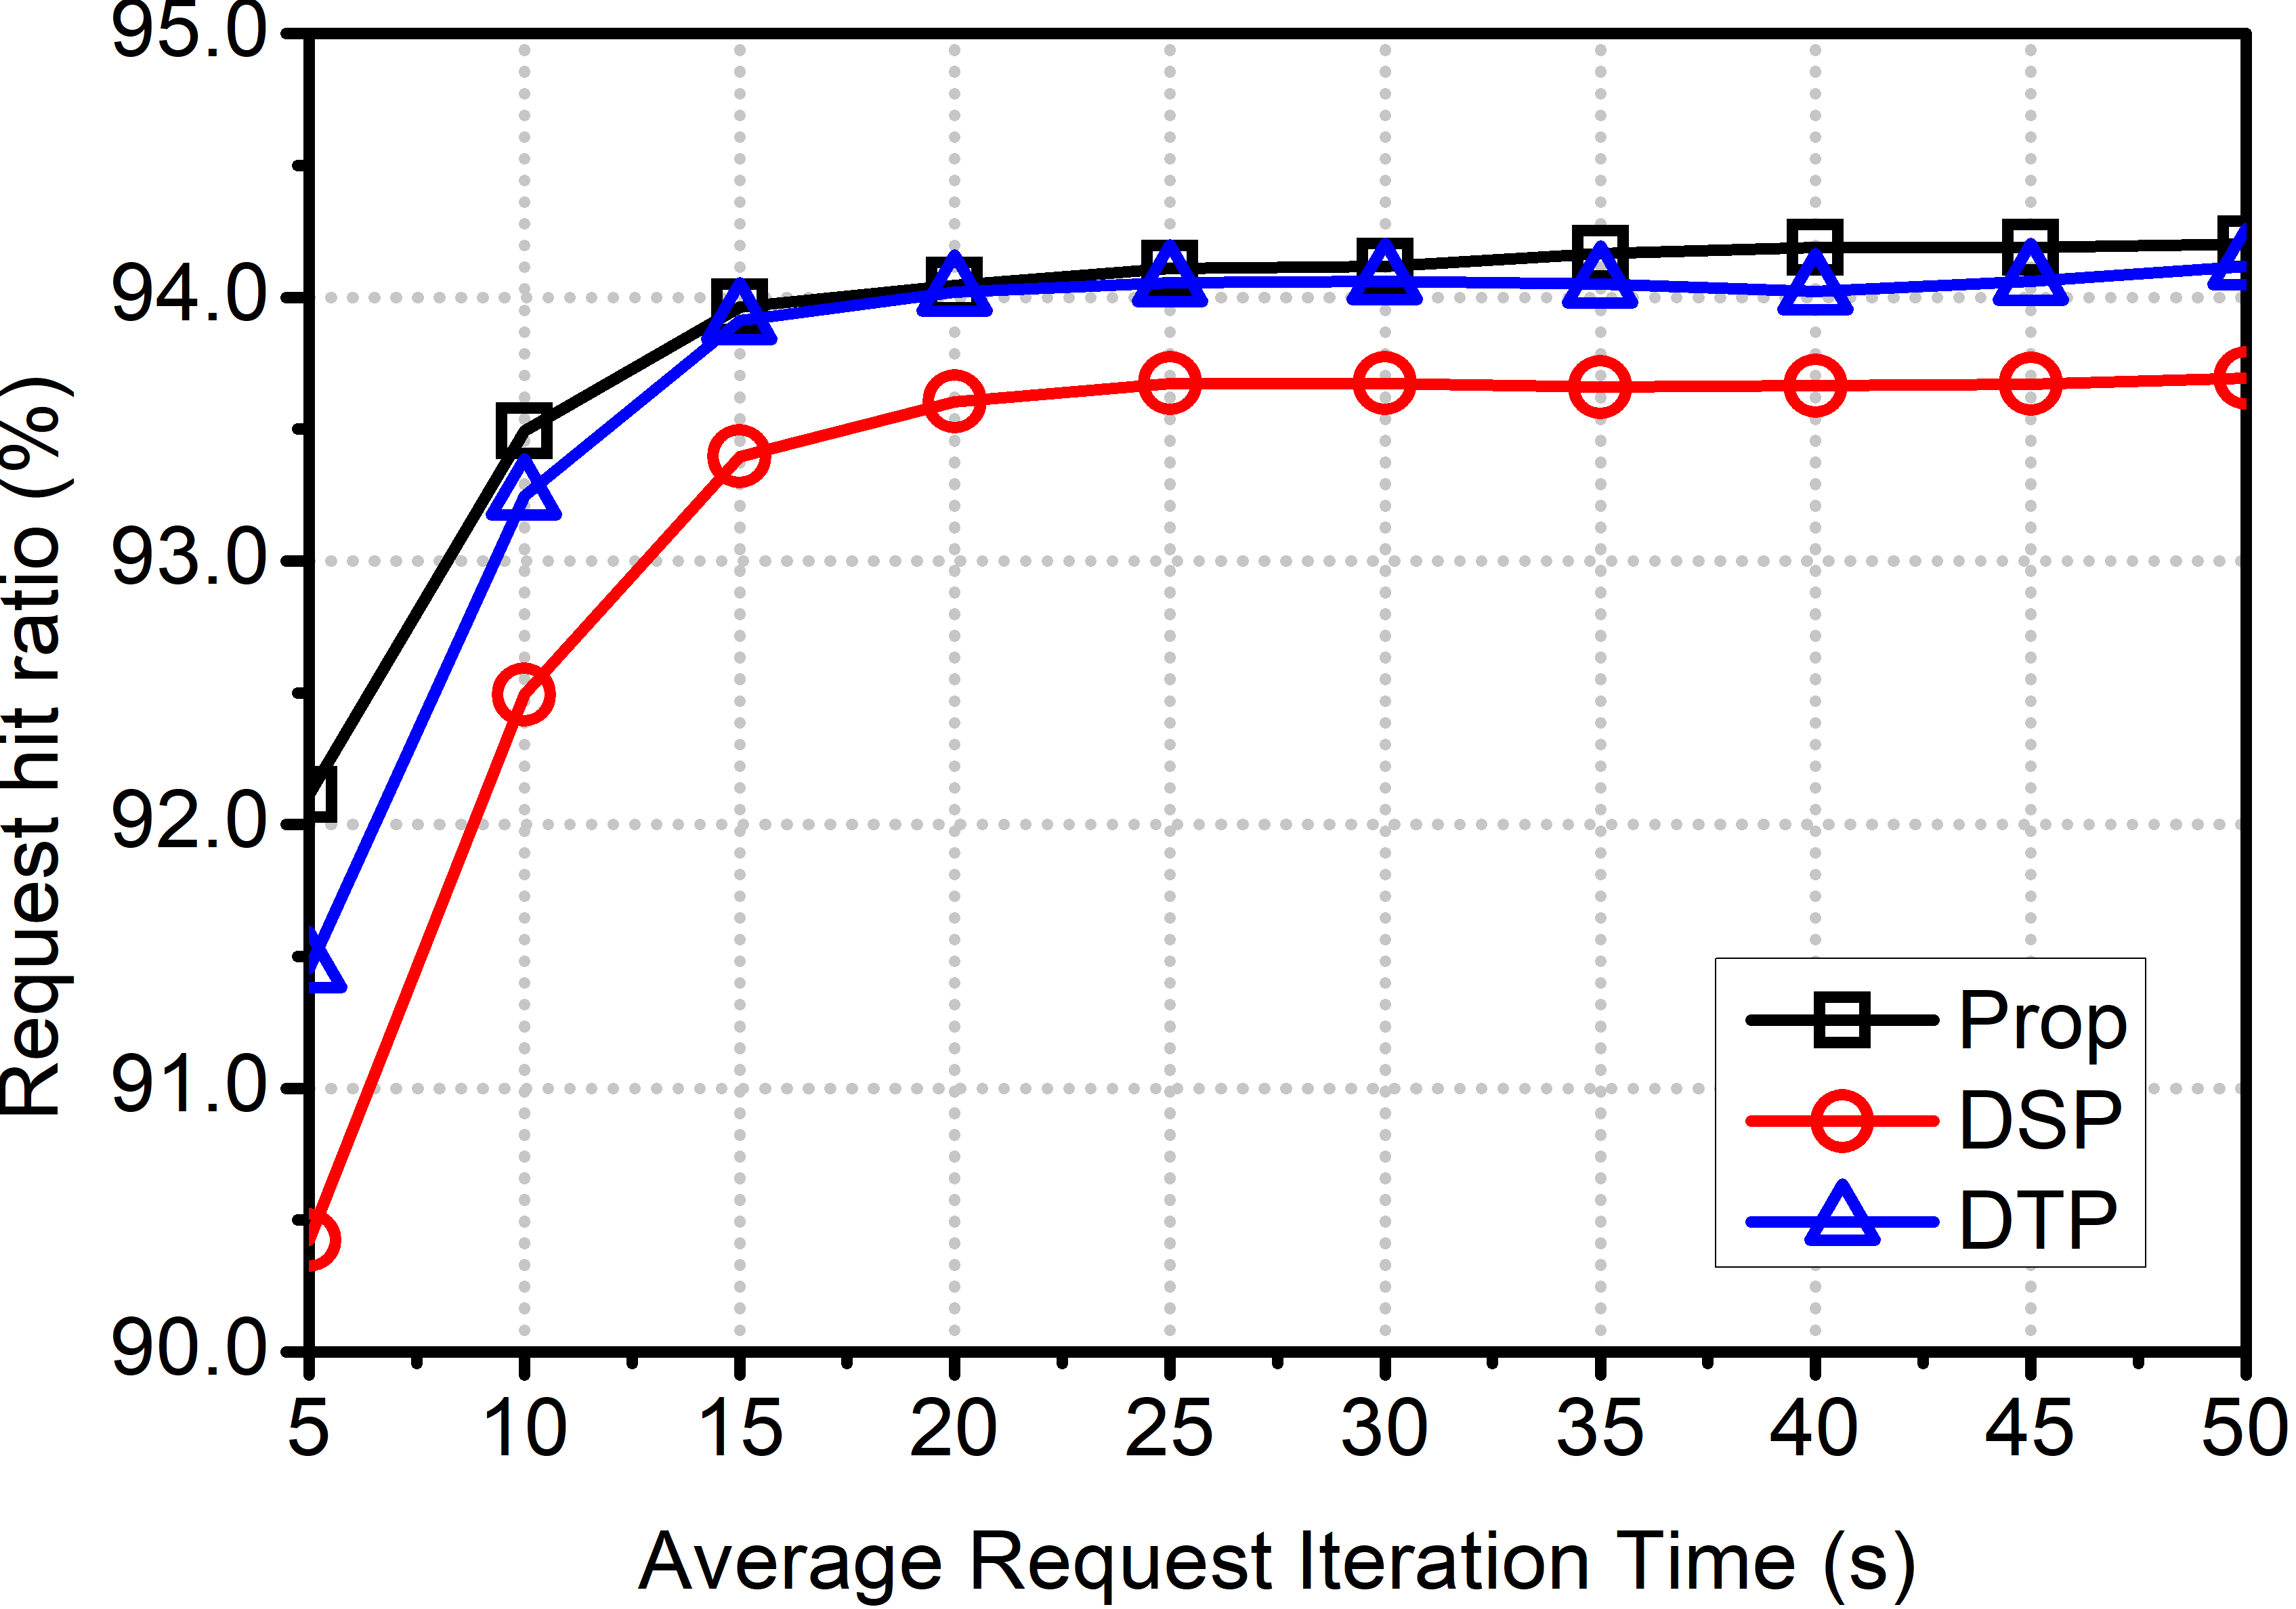
\includegraphics[width=0.325\textwidth]{./graphs/RH.png}}
    \subfigure[]{
\includegraphics[width=0.325\textwidth]{./graphs/RD.png}}
    \subfigure[]{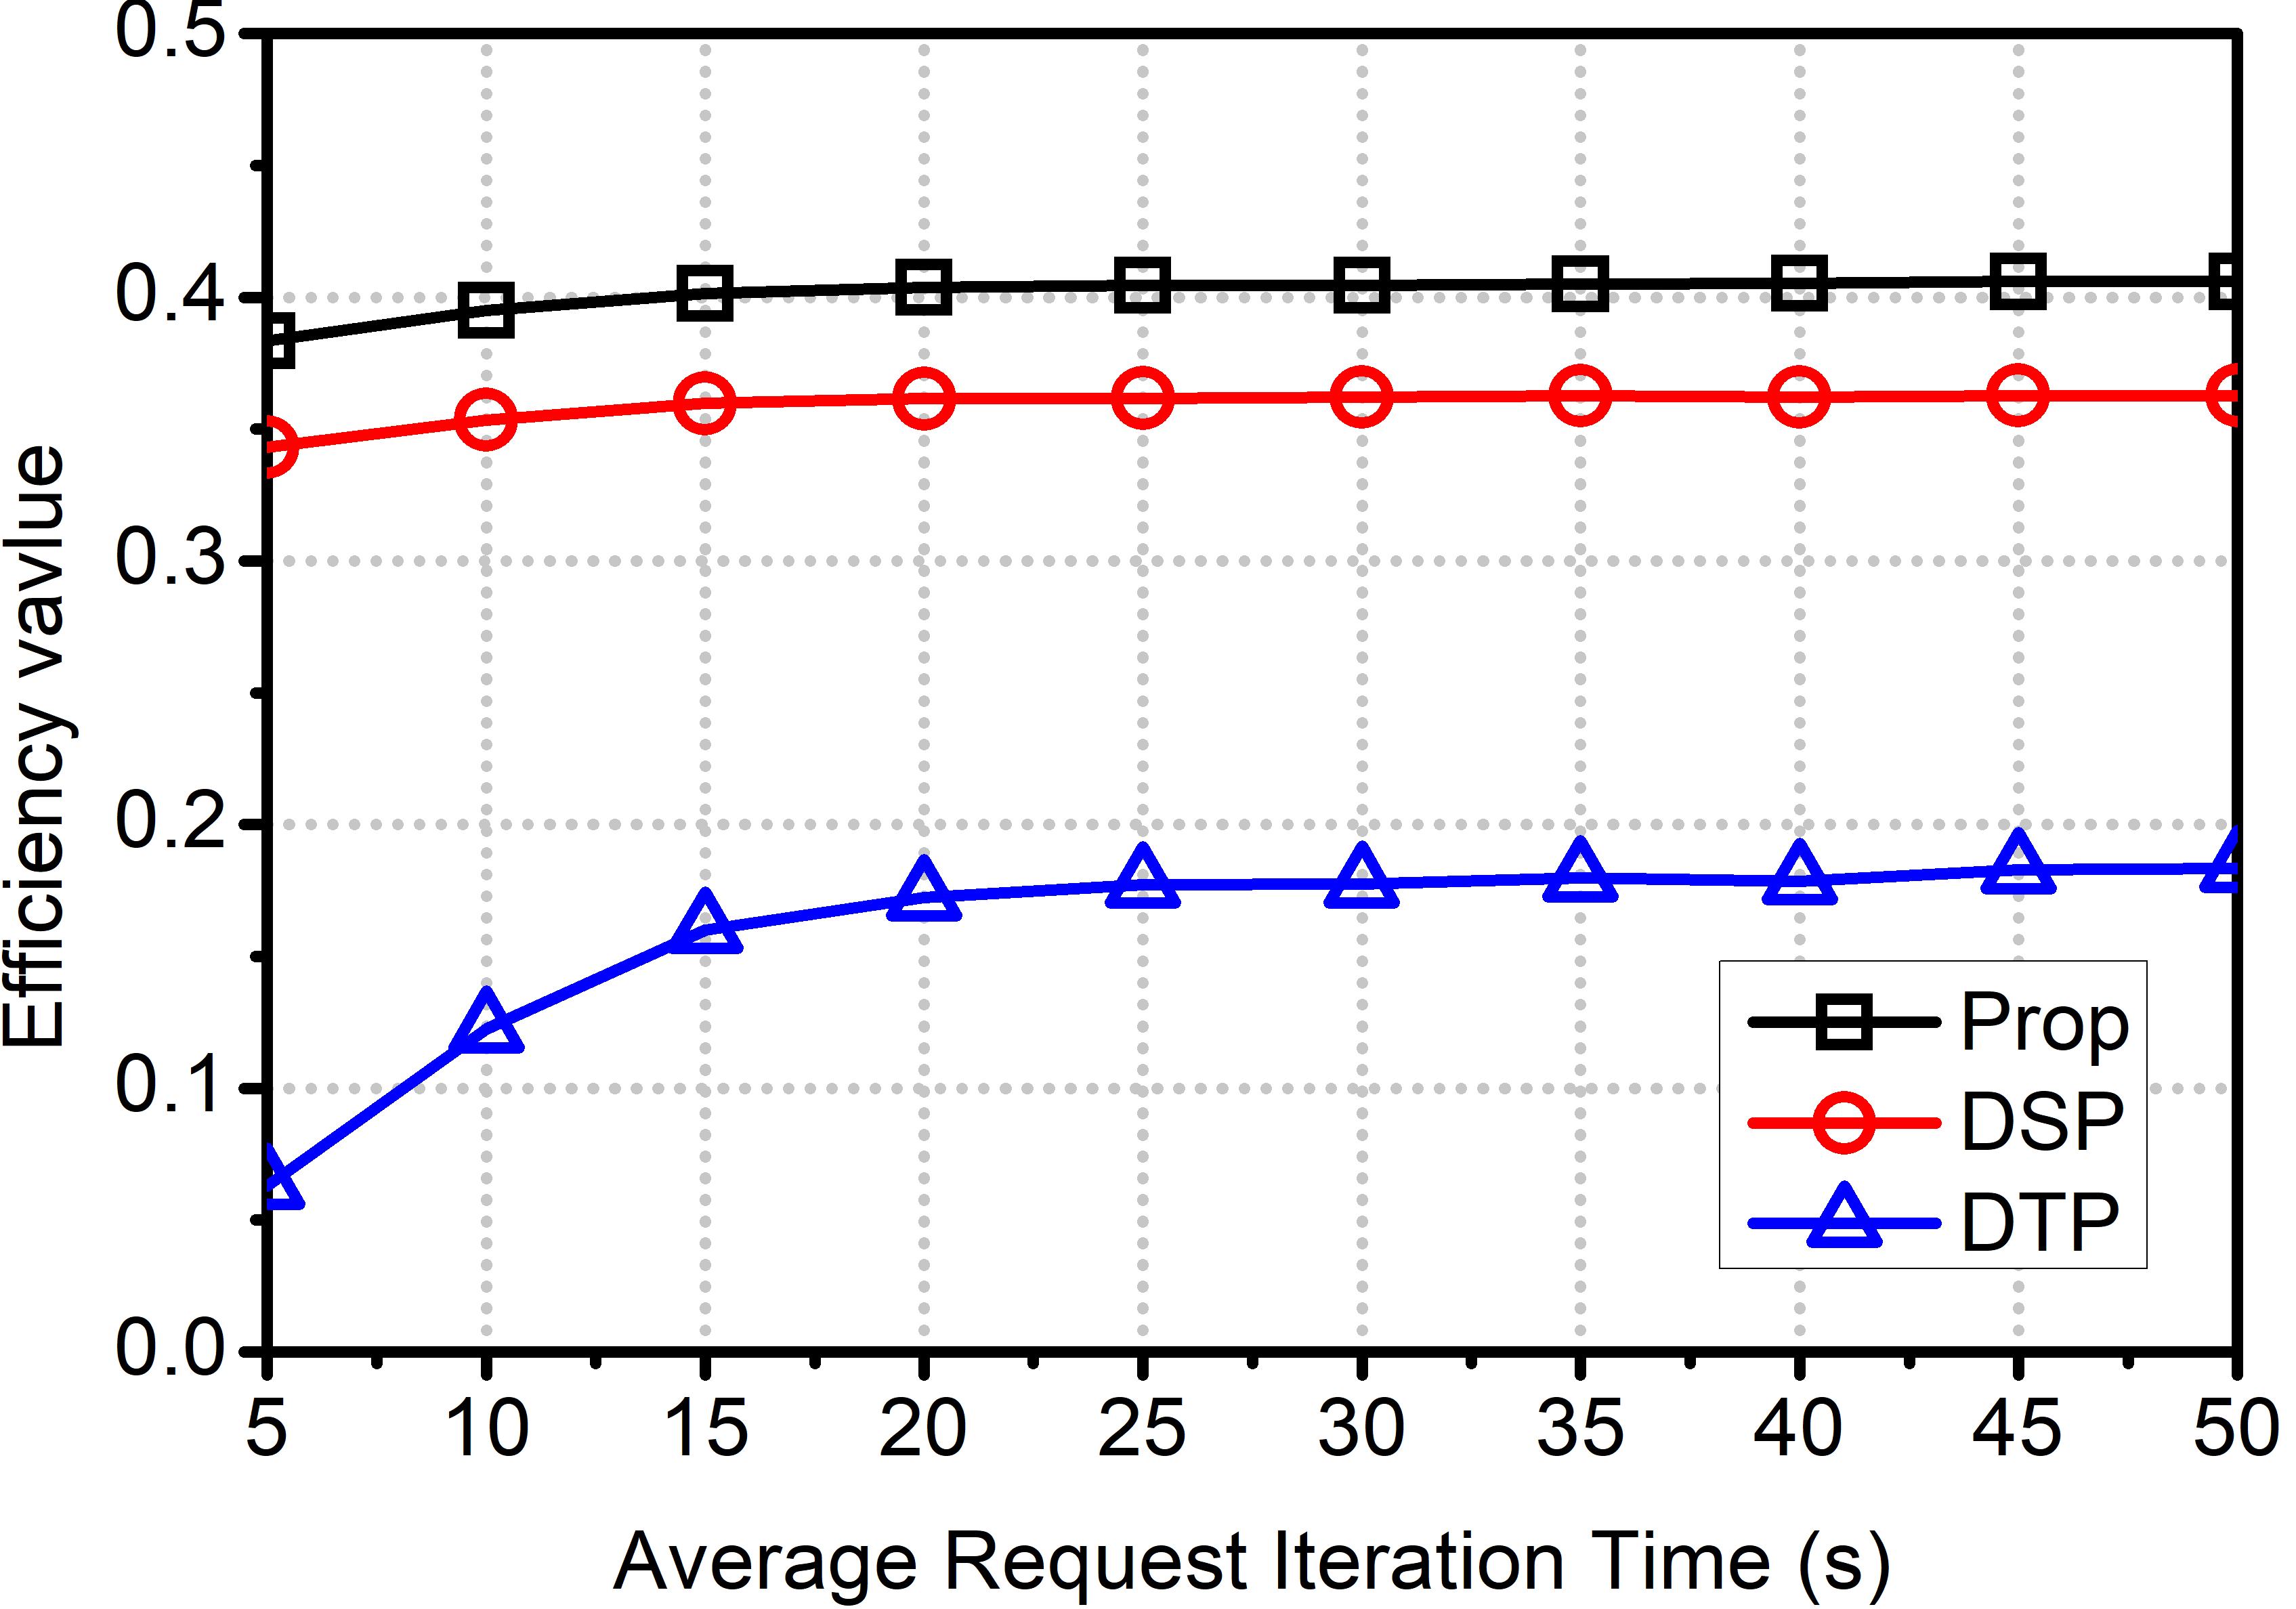
\includegraphics[width=0.325\textwidth]{./graphs/RE.png}}
    \caption{According to the average request iteration time: (a) request hit ratio; (b) content download delay; (c) efficiency value.}
    \label{fig:g1}
\end{figure*}

\subsection{Simulation Results} \label{sec.s2}
In this subsection, we will show the performances of the proposed scheme by comparing it with the other two schemes in terms of three metrics, which are the request hit ratio, content download delay, and efficiency value.
Then, for performance comparison, we implement five environmental parameters: average request iteration time, vehicle density, average vehicle speed, average content size, and average content tolerable delay.

\subsubsection{Average Request Iteration Time}
This average request iteration time is an evaluation parameter that signifies the average time interval between successive content requests from vehicles.
Each vehicle requests content at a time that is determined based on a Poisson distribution with this average.
A shorter iteration time indicates more frequent content requests, which means dynamic user interaction or a high demand for fresh content.
This metric is relevant for understanding user engagement and system load, and provides insight into the temporal dynamics of content requests.
It can affect caching strategies, with shorter iteration times leading to more content being precached or cached.
Therefore, to evaluate its performance regarding adaptation to temporal patterns in content, the average request iteration time is important.

\begin{figure*}[htp]
    \centering
    \subfigure[]{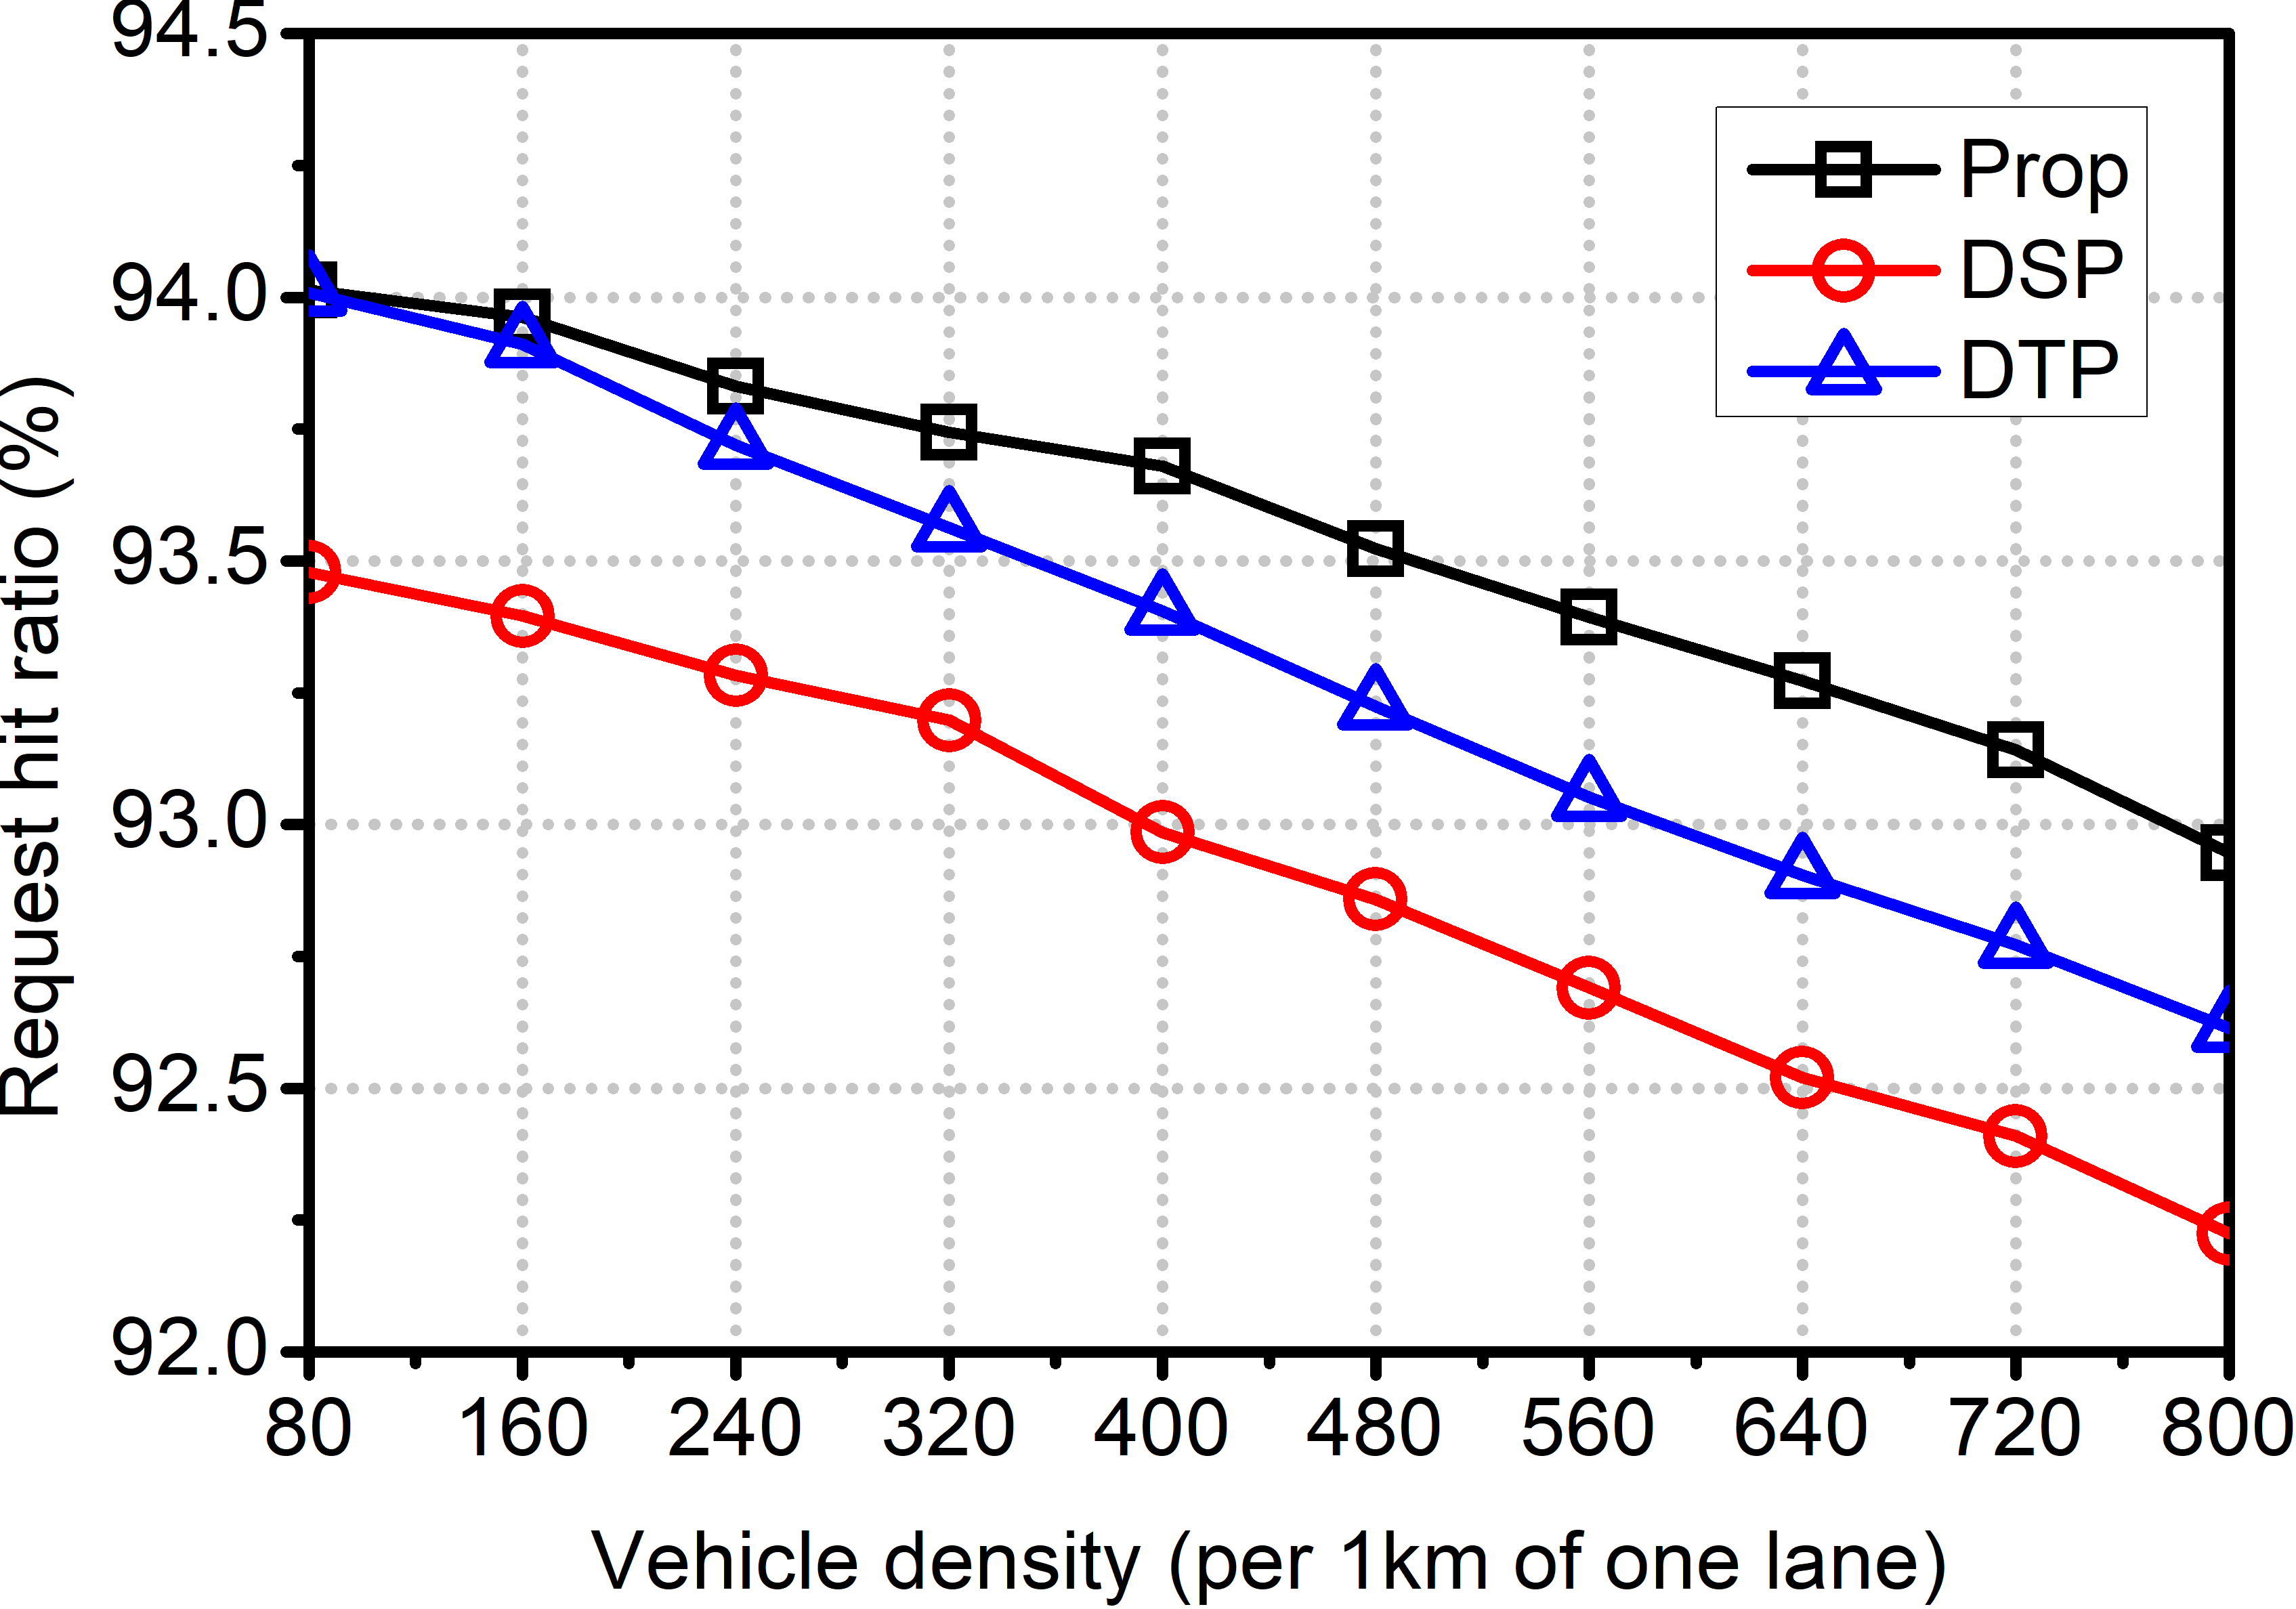
\includegraphics[width=0.325\textwidth]{./graphs/DH.png}}
    \subfigure[]{
\includegraphics[width=0.325\textwidth]{./graphs/DD.png}}
    \subfigure[]{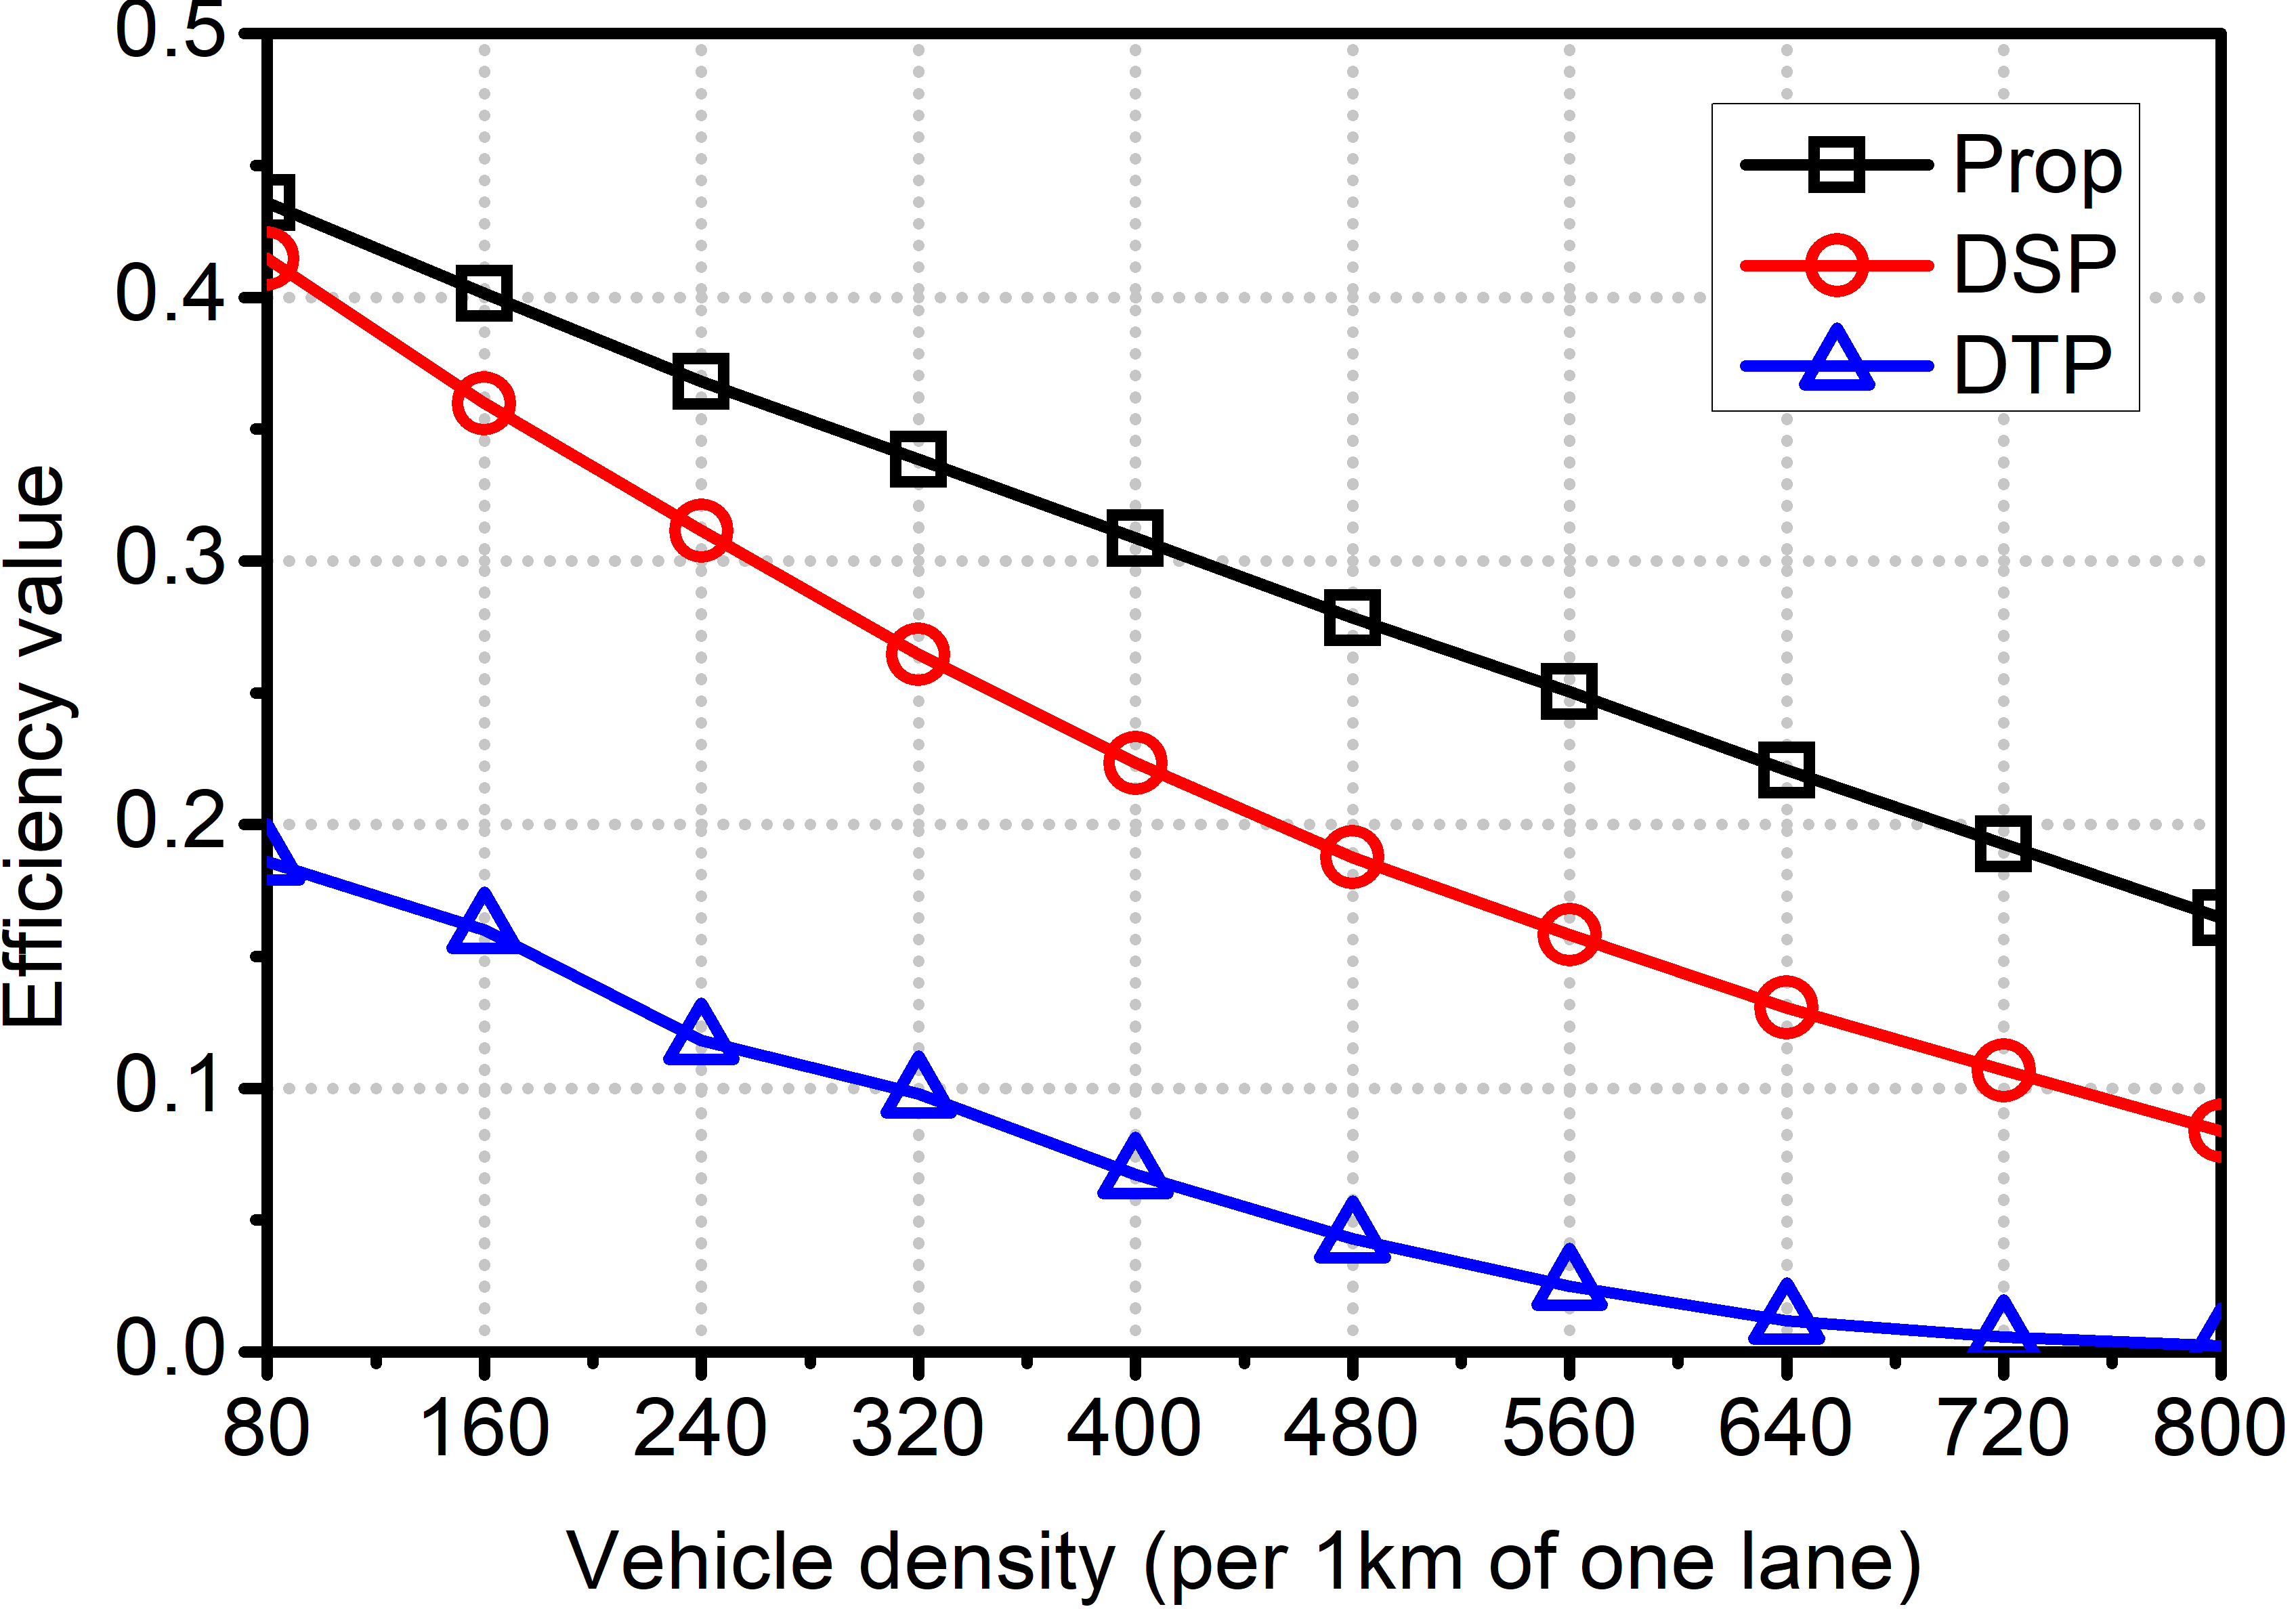
\includegraphics[width=0.325\textwidth]{./graphs/DE.png}}
    \caption{According to the vehicle density: (a) request hit ratio; (b) content download delay; (c) efficiency value.}
    \label{fig:g2}
\end{figure*}

Figure \ref{fig:g1}(a) shows the request hit ratio according to the average request iteration time.
Frequent requests for various content cause the RSUs' caching storage to cache and precache more chunks.
Therefore, cached or precached chunks are more likely to be erased because of the RSU's storage limit.
Thus, requests for the erased chunks are considered not to have been hit.
Therefore, frequent requests will decrease the request hit ratio for requests.
Because DSP does reckless precaching, more chunks are likely to be erased, resulting in the lowest request hit ratio.
Furthermore, as DTP does not precache the requested DTC, it has a higher request hit ratio compared to DSP by reducing erased chunks.
The proposed scheme improves prediction accuracy for precaching DSC by the recalculation and reduces erased chunks by utilizing cached RSUs for DTC provision, leading to the best request hit ratio.

Figure \ref{fig:g1}(b) shows the content download delay according to the average request iteration time.
As previously explained in the graph, frequent requests result in a decrease in the request hit ratio.
Un-hit requests cause backhaul link traffic.
Due to limited resources on the backhaul links, heavy traffic can cause scheduling delays.
Also, the un-hit requests may be resolved by bringing the requested chunks from the other RSUs or the content server, resulting in access delay.
Therefore, frequent requests cause more content download delay.
Since DSP has the lowest hit ratio, it has the largest content download delay.
Since the proposed scheme has a better hit ratio than DTP, it has a minimum content download delay.

Figure \ref{fig:g1}(c) shows the efficiency value according to the average request iteration time.
Erased chunks from cached RUs affect the success ratio for DTC download because DTC is provided from cached RSUs.
Also, delays within cached RSUs can cause the time to complete content download to exceed the tolerable delay.
Thus, frequent requests cause erased chunks and delays, reducing the success ratio.
Especially, DTP has a very low success ratio because it doesn't precache the DTC chunks because it doesn't consider the tolerable delay.
Although it consumes very little traffic, it has the lowest efficiency value because its success ratio is too low.
Conversely, DSP has a very high ratio because it precaches all the chunks of DTC by not considering the content tolerance characteristics.
However, since it consumes too much traffic to precache all the chunks that are not cached, it has a lower efficiency value than the proposed scheme.

\begin{figure*}[htp]
    \centering
    \subfigure[]{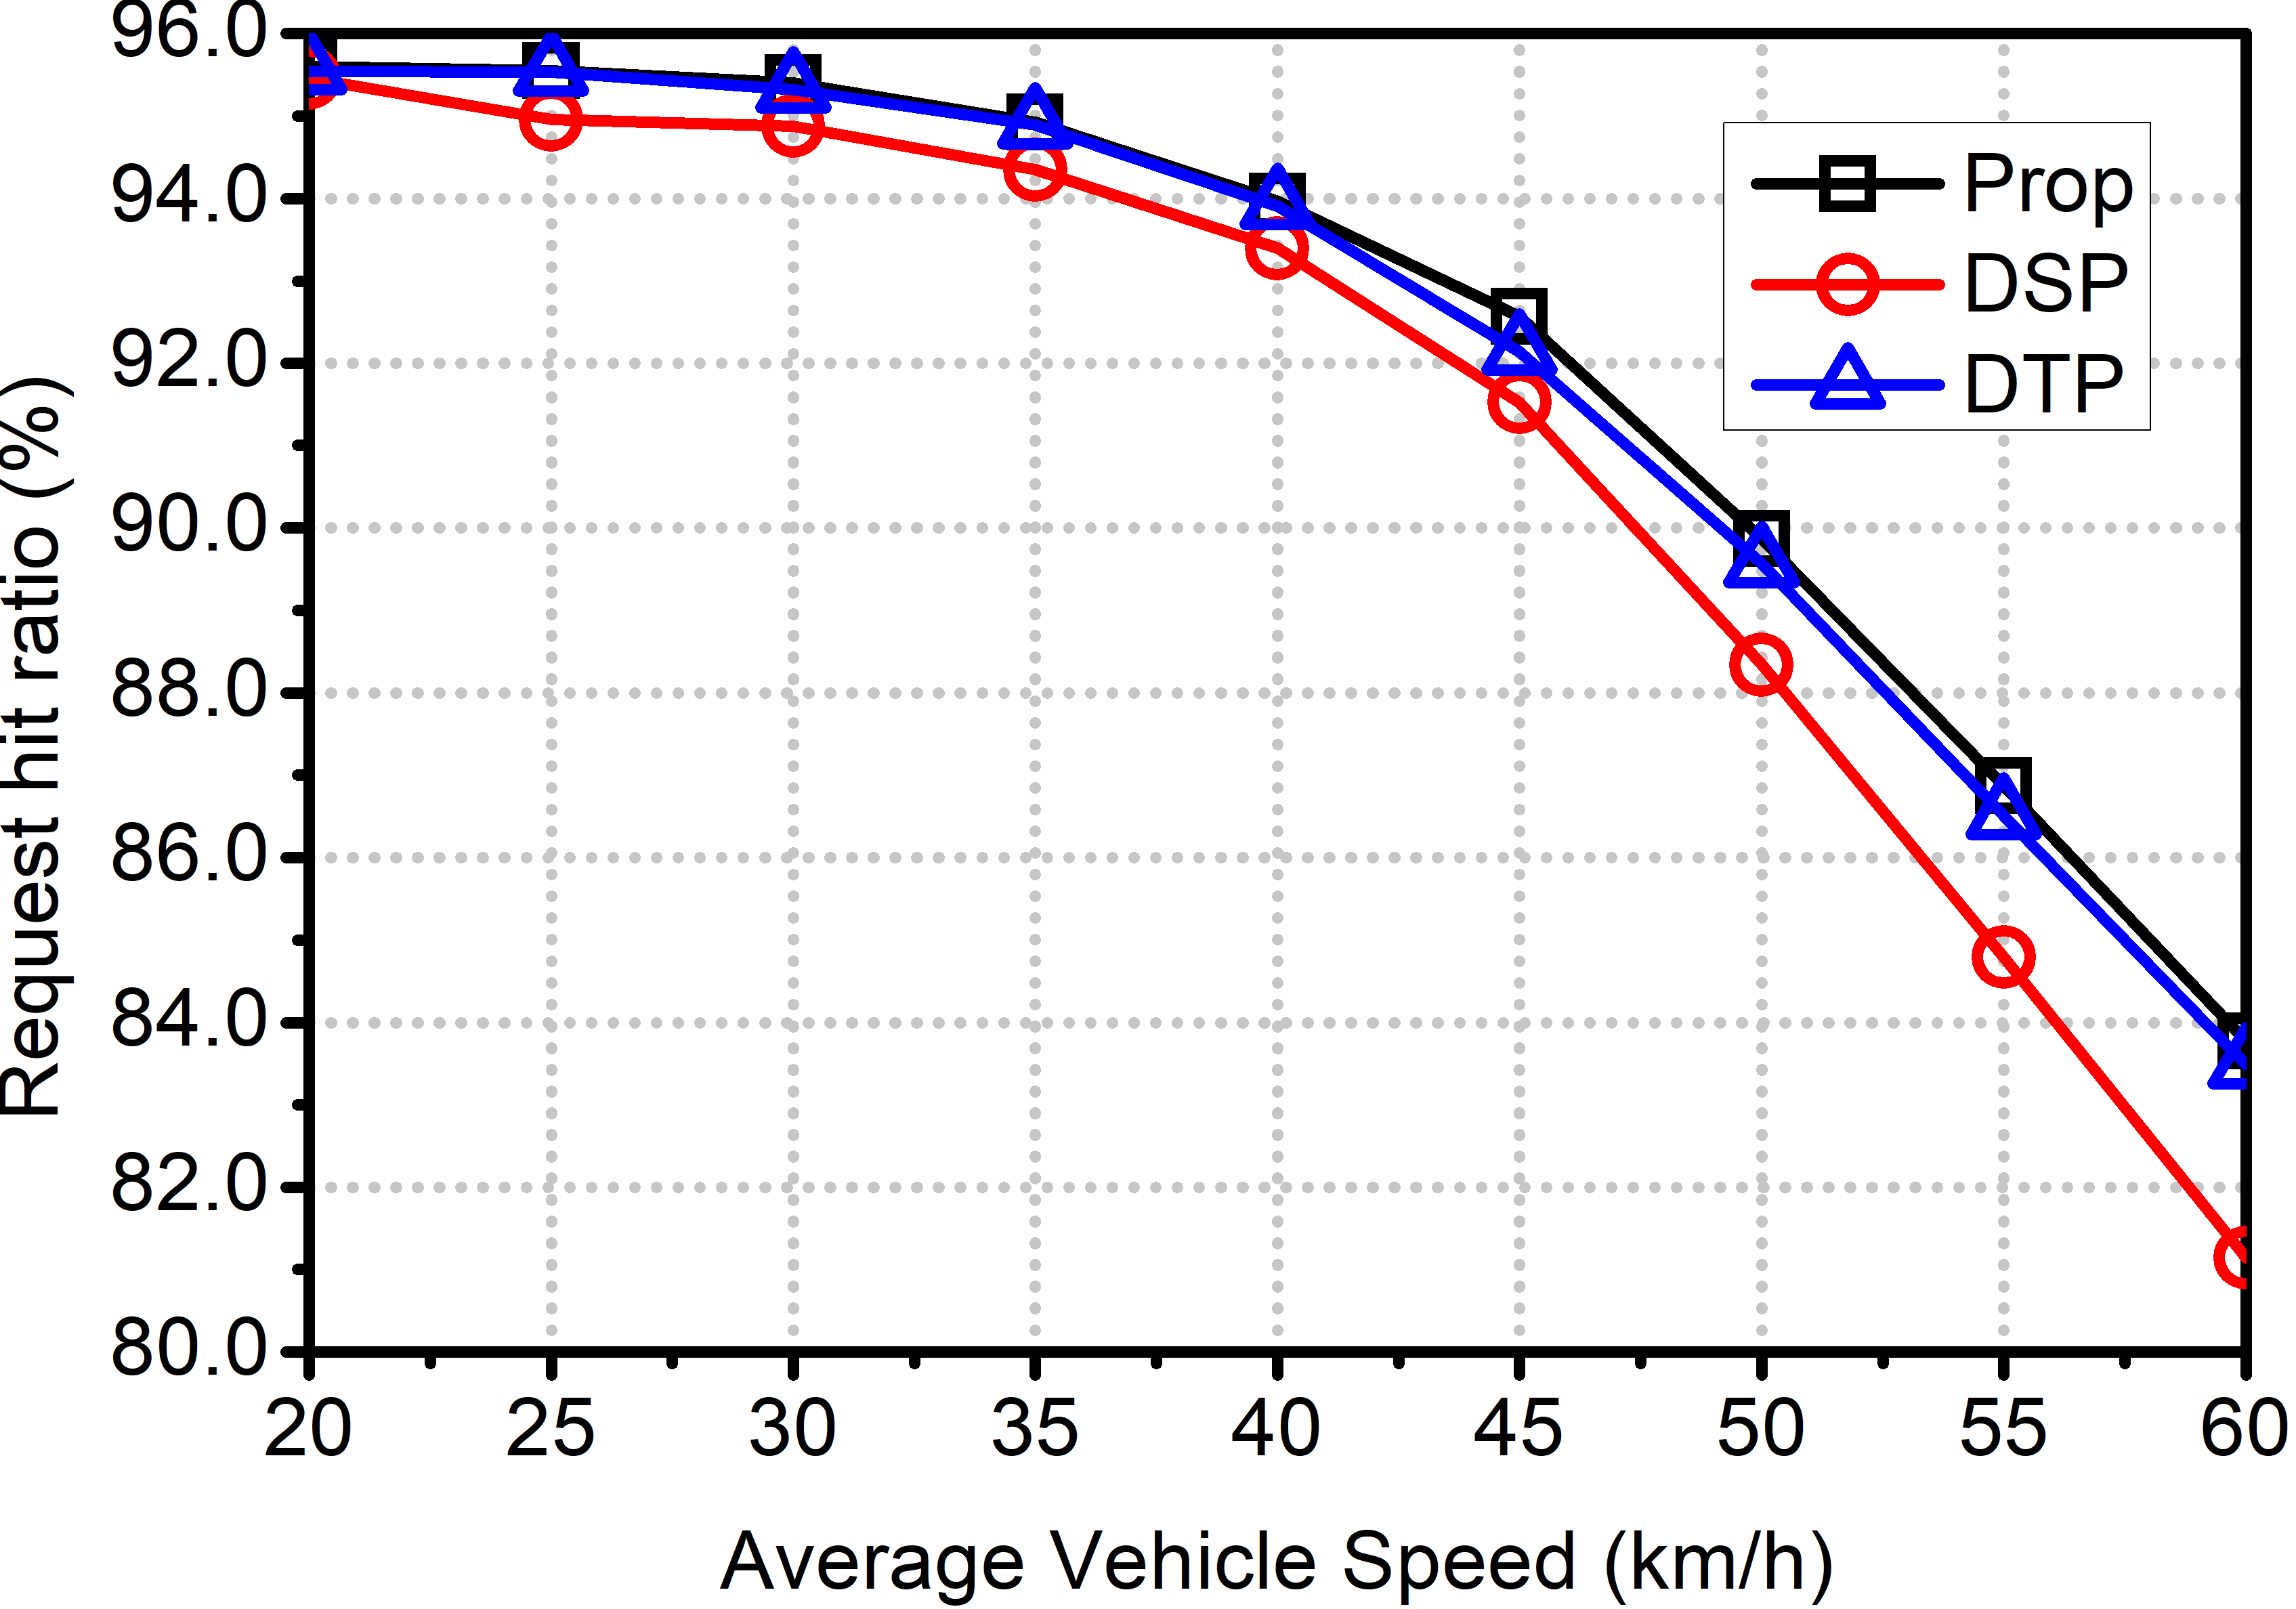
\includegraphics[width=0.325\textwidth]{./graphs/VH.png}}
    \subfigure[]{
\includegraphics[width=0.325\textwidth]{./graphs/VD.png}}
    \subfigure[]{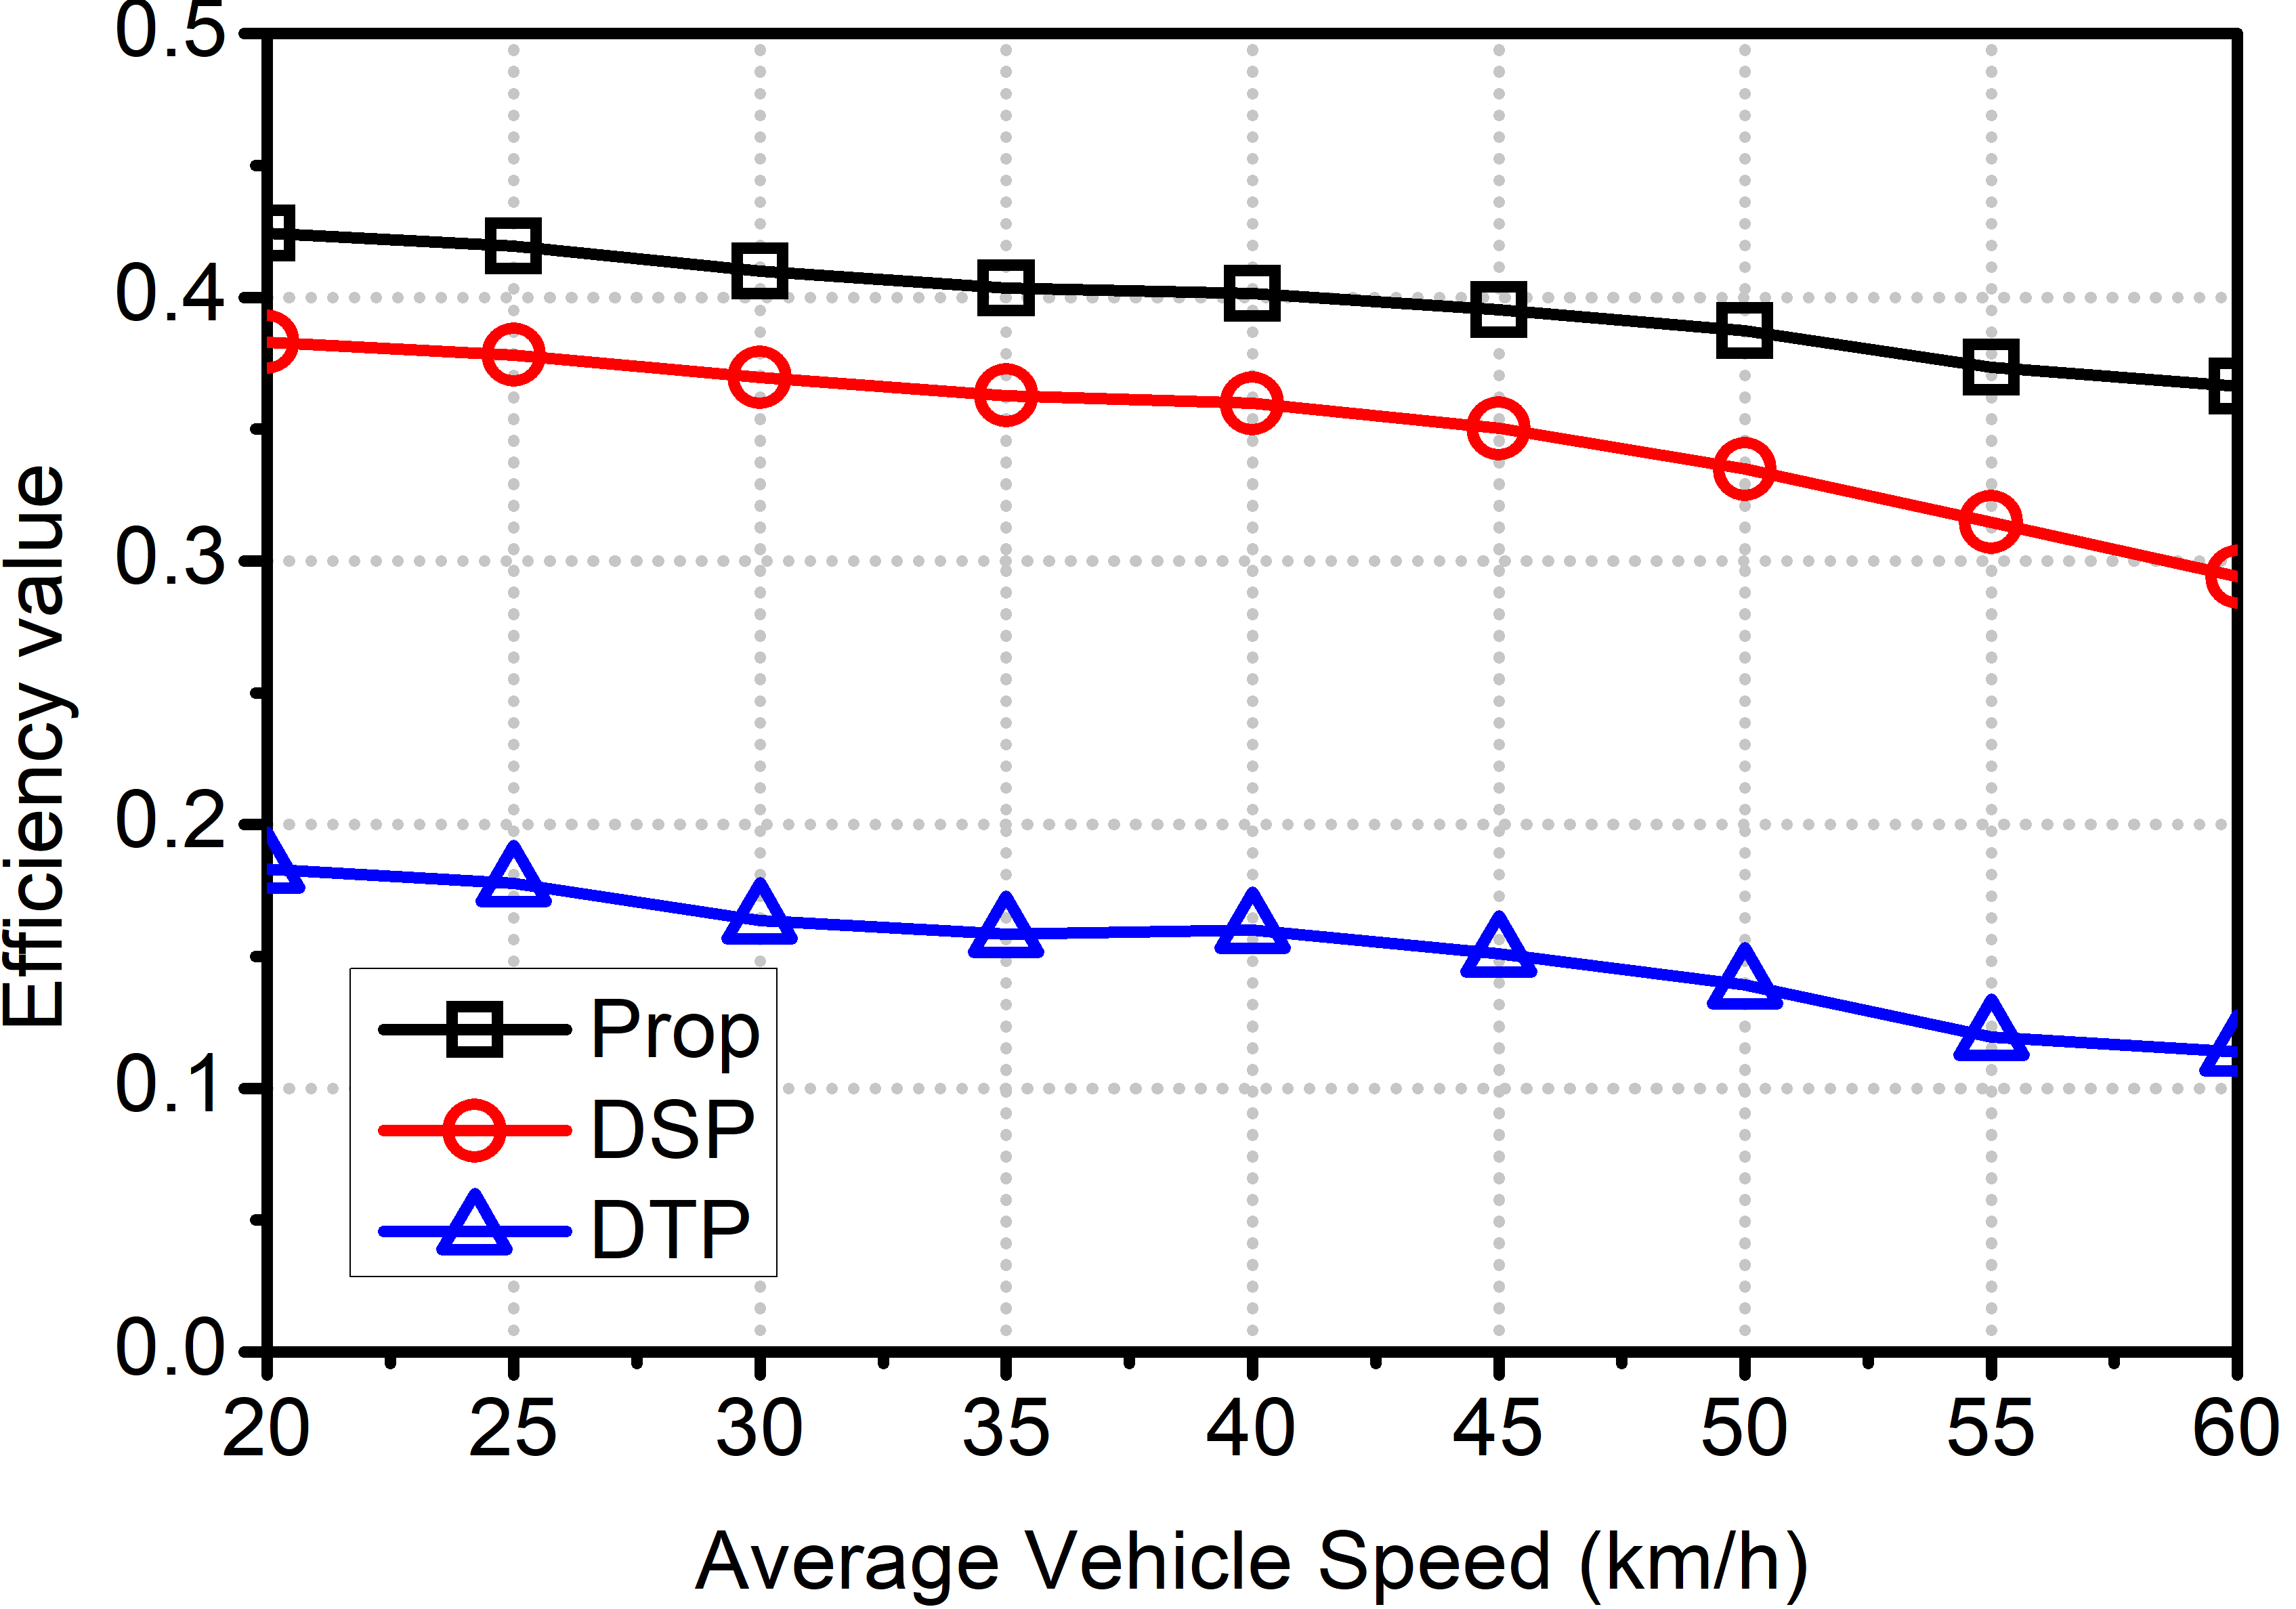
\includegraphics[width=0.325\textwidth]{./graphs/VE.png}}
    \caption{According to the average vehicle speed: (a) request hit ratio; (b) content download delay; (c) efficiency value.}
    \label{fig:g3}
\end{figure*}

\subsubsection{Vehicle density}
Vehicle density is an evaluation parameter that characterizes the concentration of vehicles within a network area, typically expressed as the number of vehicles per 1km of one lane.
When evaluating content delivery performance, vehicle density provides critical insight into traffic and interaction patterns within the network.
High vehicle density indicates a more congested environment, which can lead to increased contention for network resources, such as RSU radio resources or backhaul links.
Higher densities of this parameter can affect the efficiency of content delivery, which requires more robust caching and delivery mechanisms to handle concurrent requests.
Therefore, vehicle density is an important consideration in evaluating its performance in adapting to spatial content patterns.

Figure \ref{fig:g2}(a) shows the request hit ratio according to the vehicle density.
As vehicle density increases, the frequency of content requests also increases, potentially leading to a faster turnover of cached and precached content in the RSU's caching storage.
With limited storage capacity, RSUs may struggle to retain all requested content, resulting in a lower hit ratio.
Frequent and varied requests can cause older or less popular content to be continually replaced, making it less likely that a new request will match existing cached content by providing and precaching more requested content.
Because DSP caches more chunks through reckless precaching, this problem is worse, resulting in the lowest hit ratio.
Since DTP can reduce precaching chunks, but the proposed scheme has better prediction accuracy for precaching DSC, the proposed scheme has the best hit ratio.

Figure \ref{fig:g2}(b) shows the content download delay according to the vehicle density.
The higher density of vehicles causes a higher turnover of cached and precached content in RSUs, which can cause unexpected erases.
When important content is erased, the request for the content can cause repeated traffic consumption on backhaul links.
In addition, as vehicle density increases, the number of content requests increases, resulting in more traffic on the backhaul links.
The increased traffic can cause scheduling delays due to resource competition within RSUs and on backhaul links.
Since DSP consumes more traffic due to reckless precaching, it has the highest content download delay.
In the proposed scheme, by improving the prediction accuracy and preventing the erases of important content, the content download delay is the lowest then the other two schemes.

Figure \ref{fig:g2}(c) shows the efficiency value according to the vehicle density.
As the number of vehicles on the road increases, the number of content requests also increases.
This increased demand can lead to more frequent requests for content, which in turn can strain available resources such as RSU caching storage and backhaul links.
The increased competition for resources among vehicles could result in more content being erased from the caching storage, which is directly related to the success rate of DTC download within its tolerable delay.
Therefore, even though DTP doesn't consume any backhaul link traffic for precaching DTC, it has the lowest efficiency value because its success rate is too low.
Conversely, although DSP has the highest success ratio and the lowest download delay due to the reckless precaching of DTC, it has a lower efficiency value than the proposed scheme because it consumes too much backhaul link traffic.

\begin{figure*}[htp]
    \centering
    \subfigure[]{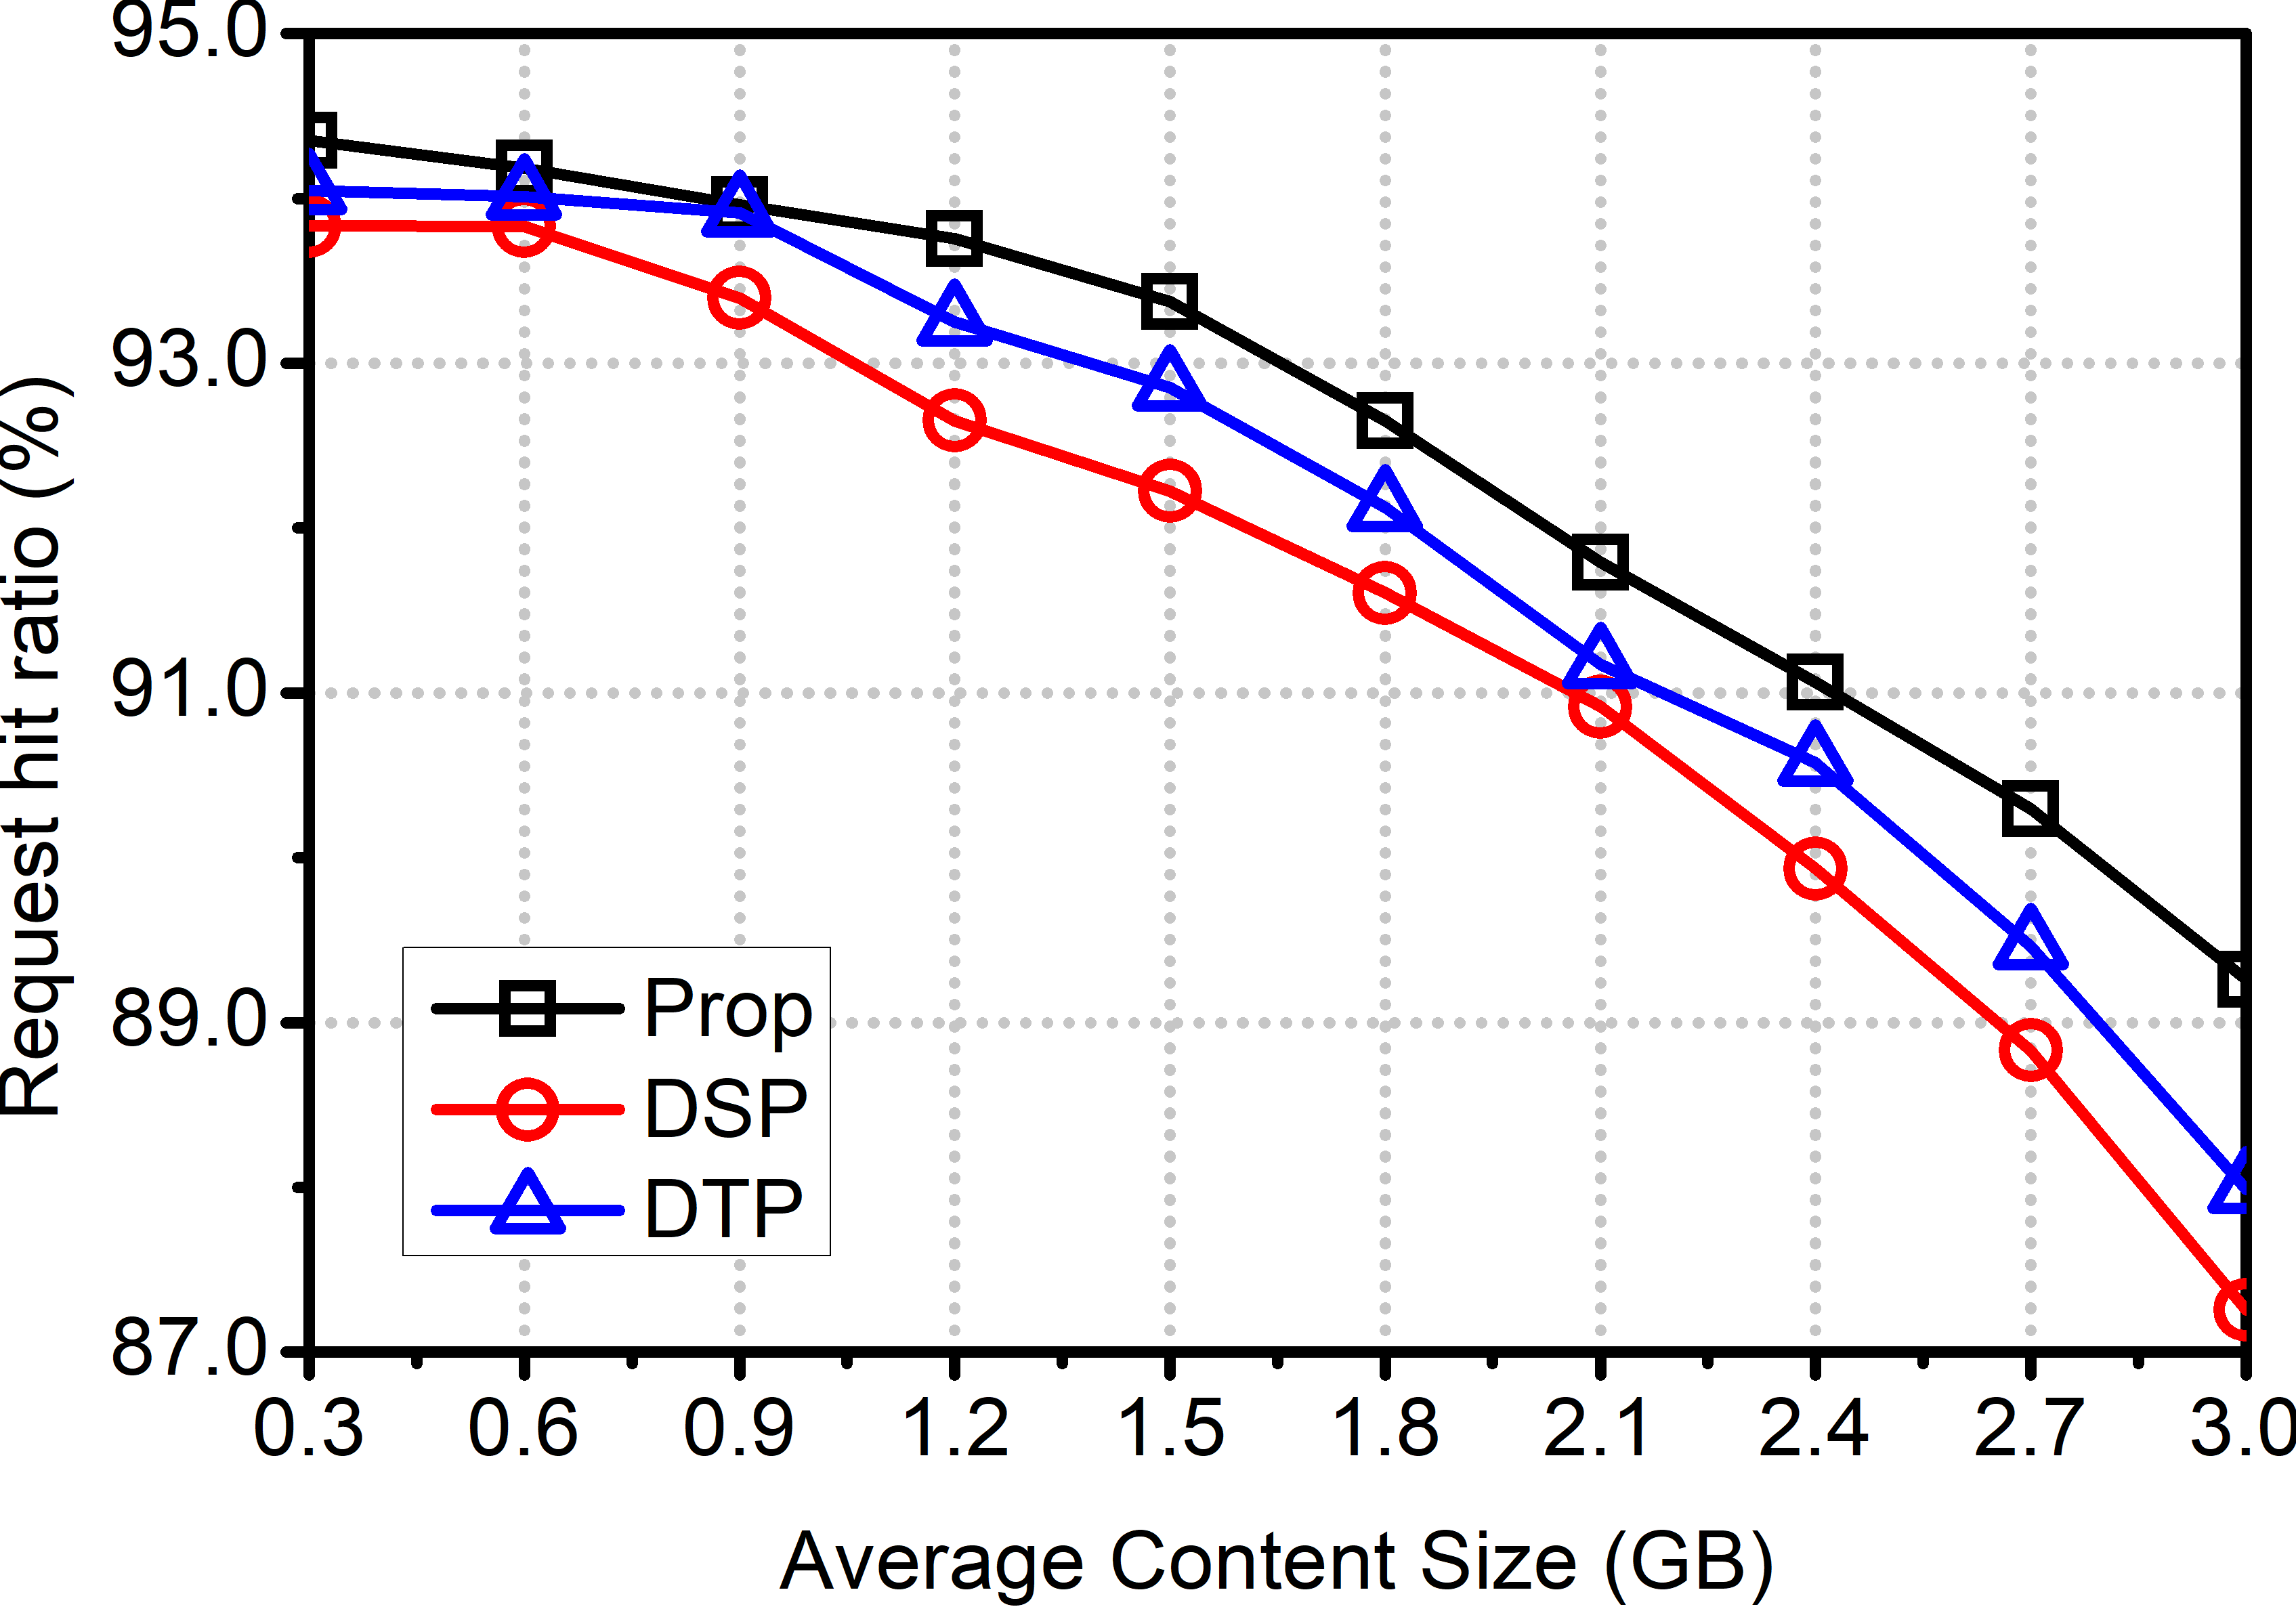
\includegraphics[width=0.325\textwidth]{./graphs/SH.png}}
    \subfigure[]{
\includegraphics[width=0.325\textwidth]{./graphs/SD.png}}
    \subfigure[]{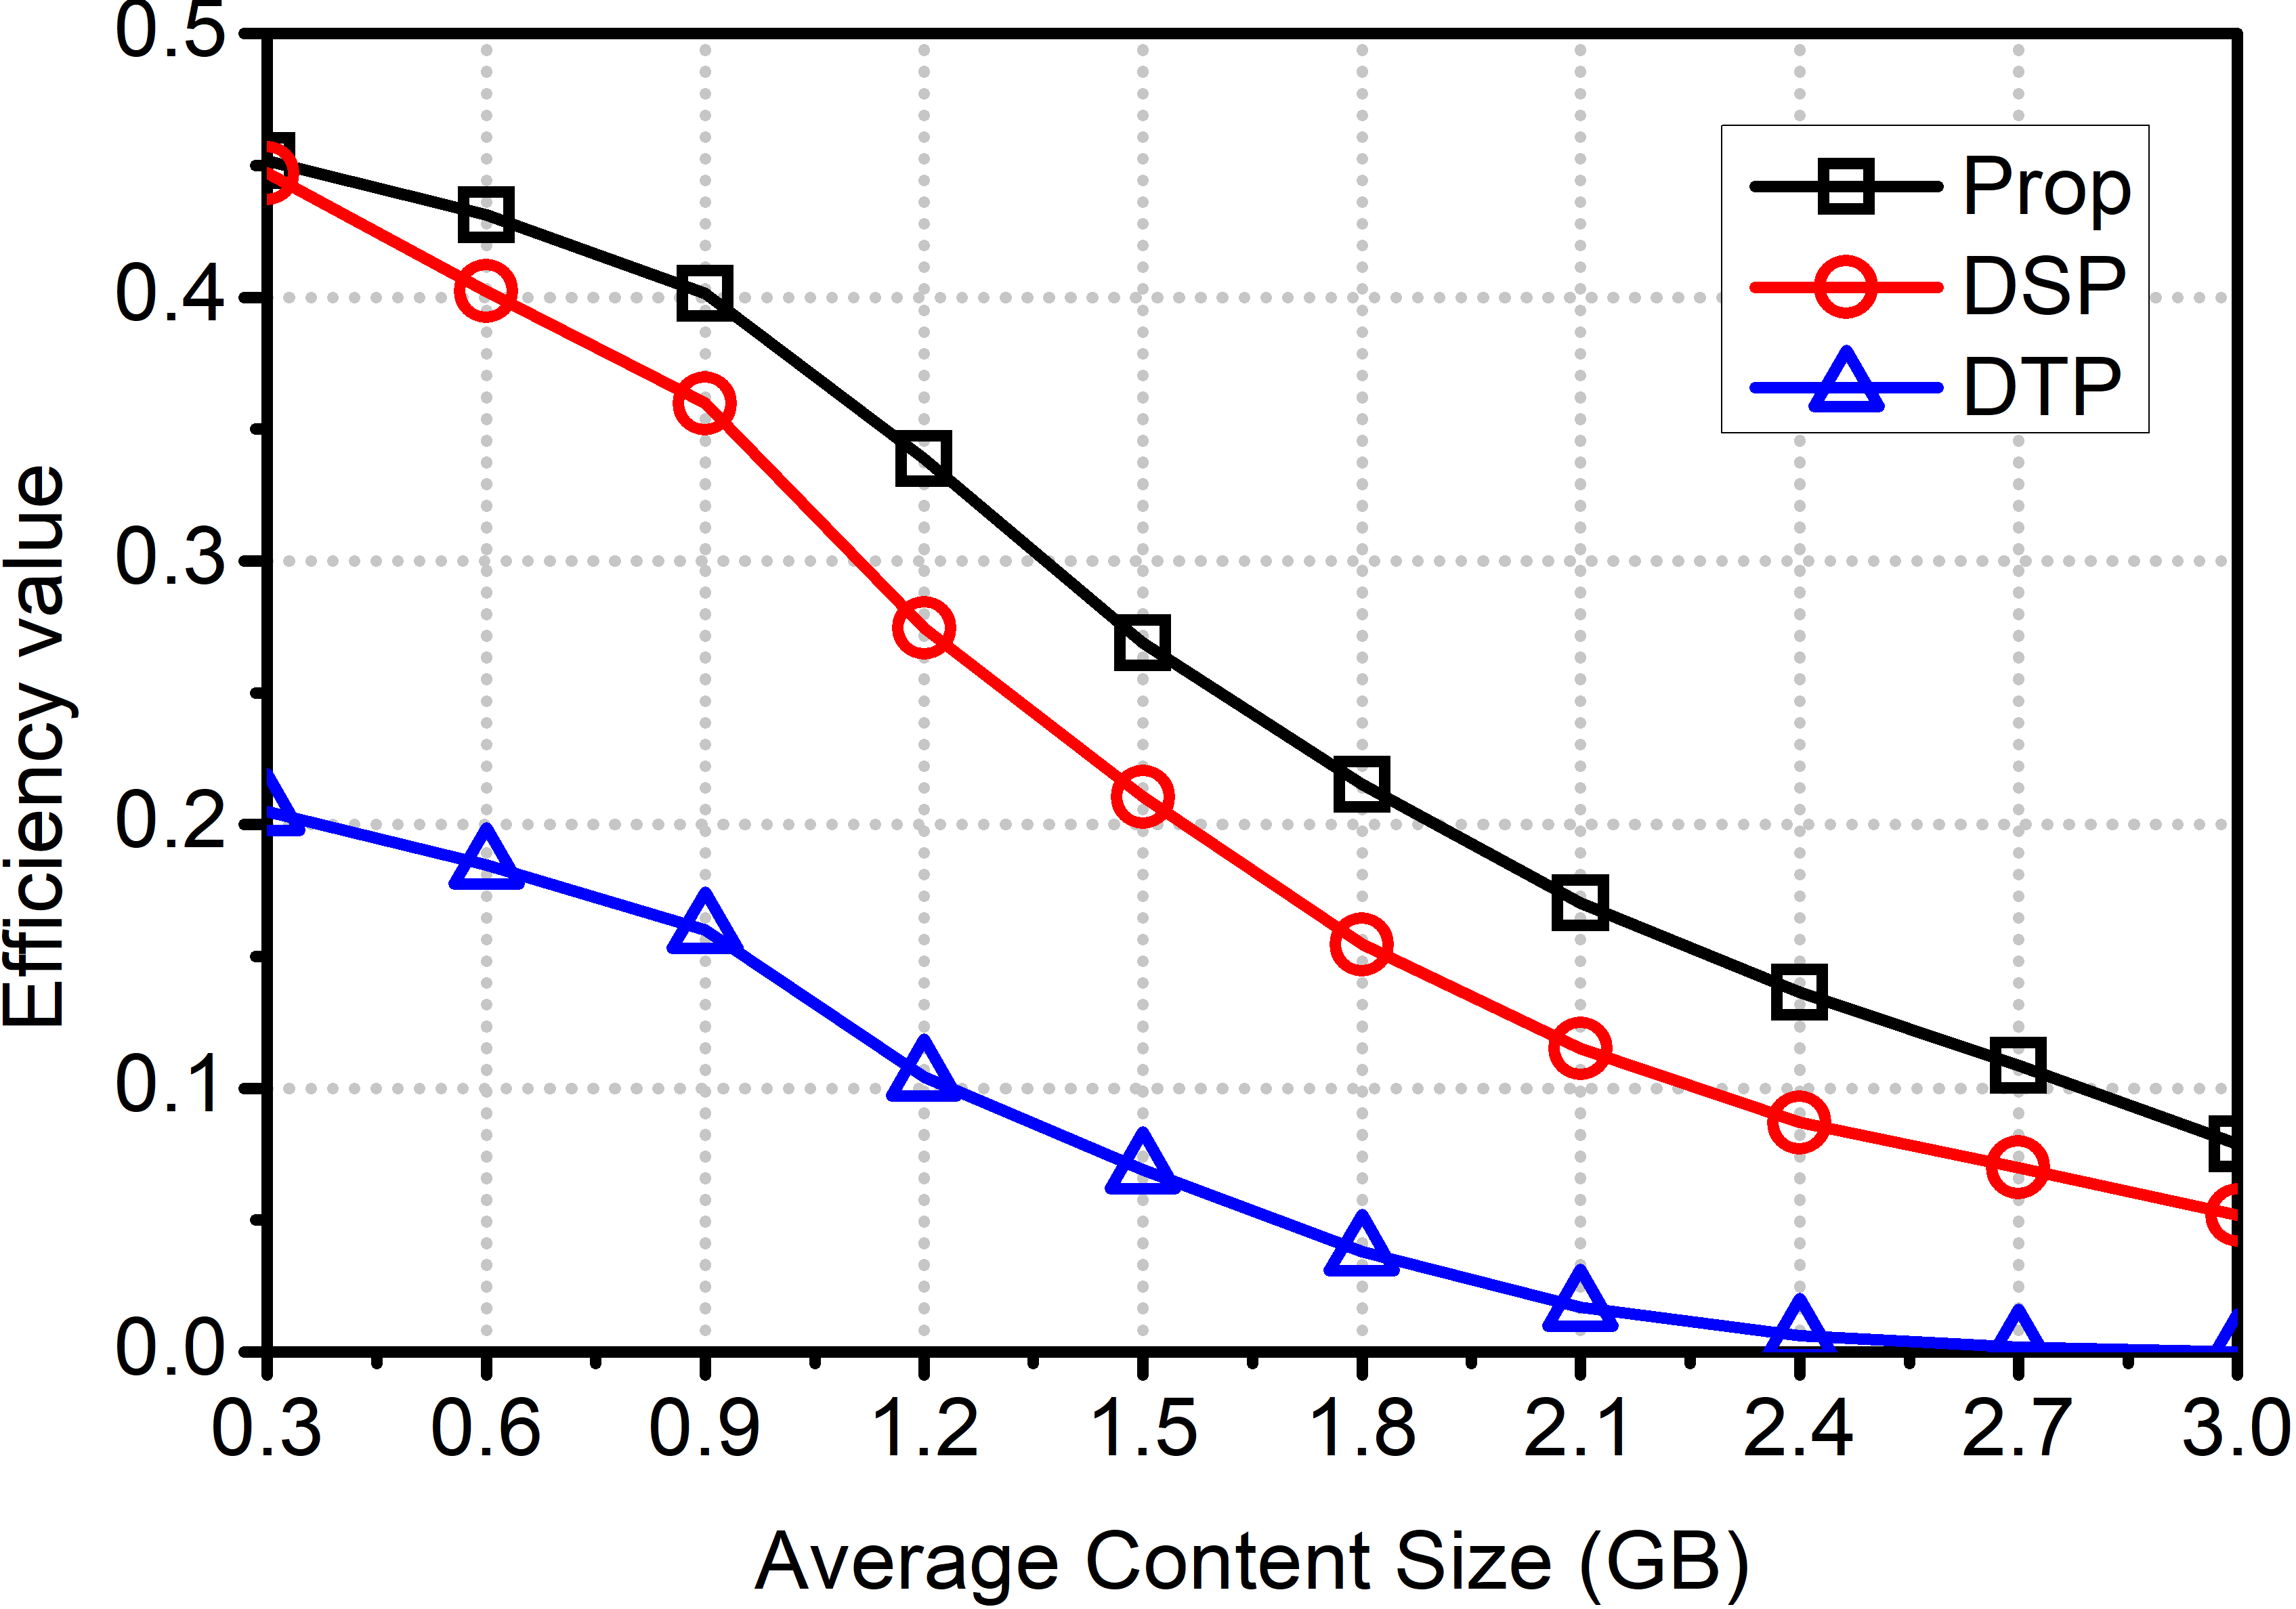
\includegraphics[width=0.325\textwidth]{./graphs/SE.png}}
    \caption{According to the average content size: (a) request hit ratio; (b) content download delay; (c) efficiency value.}
    \label{fig:g4}
\end{figure*}

\begin{figure*}[htp]
    \centering
    \subfigure[]{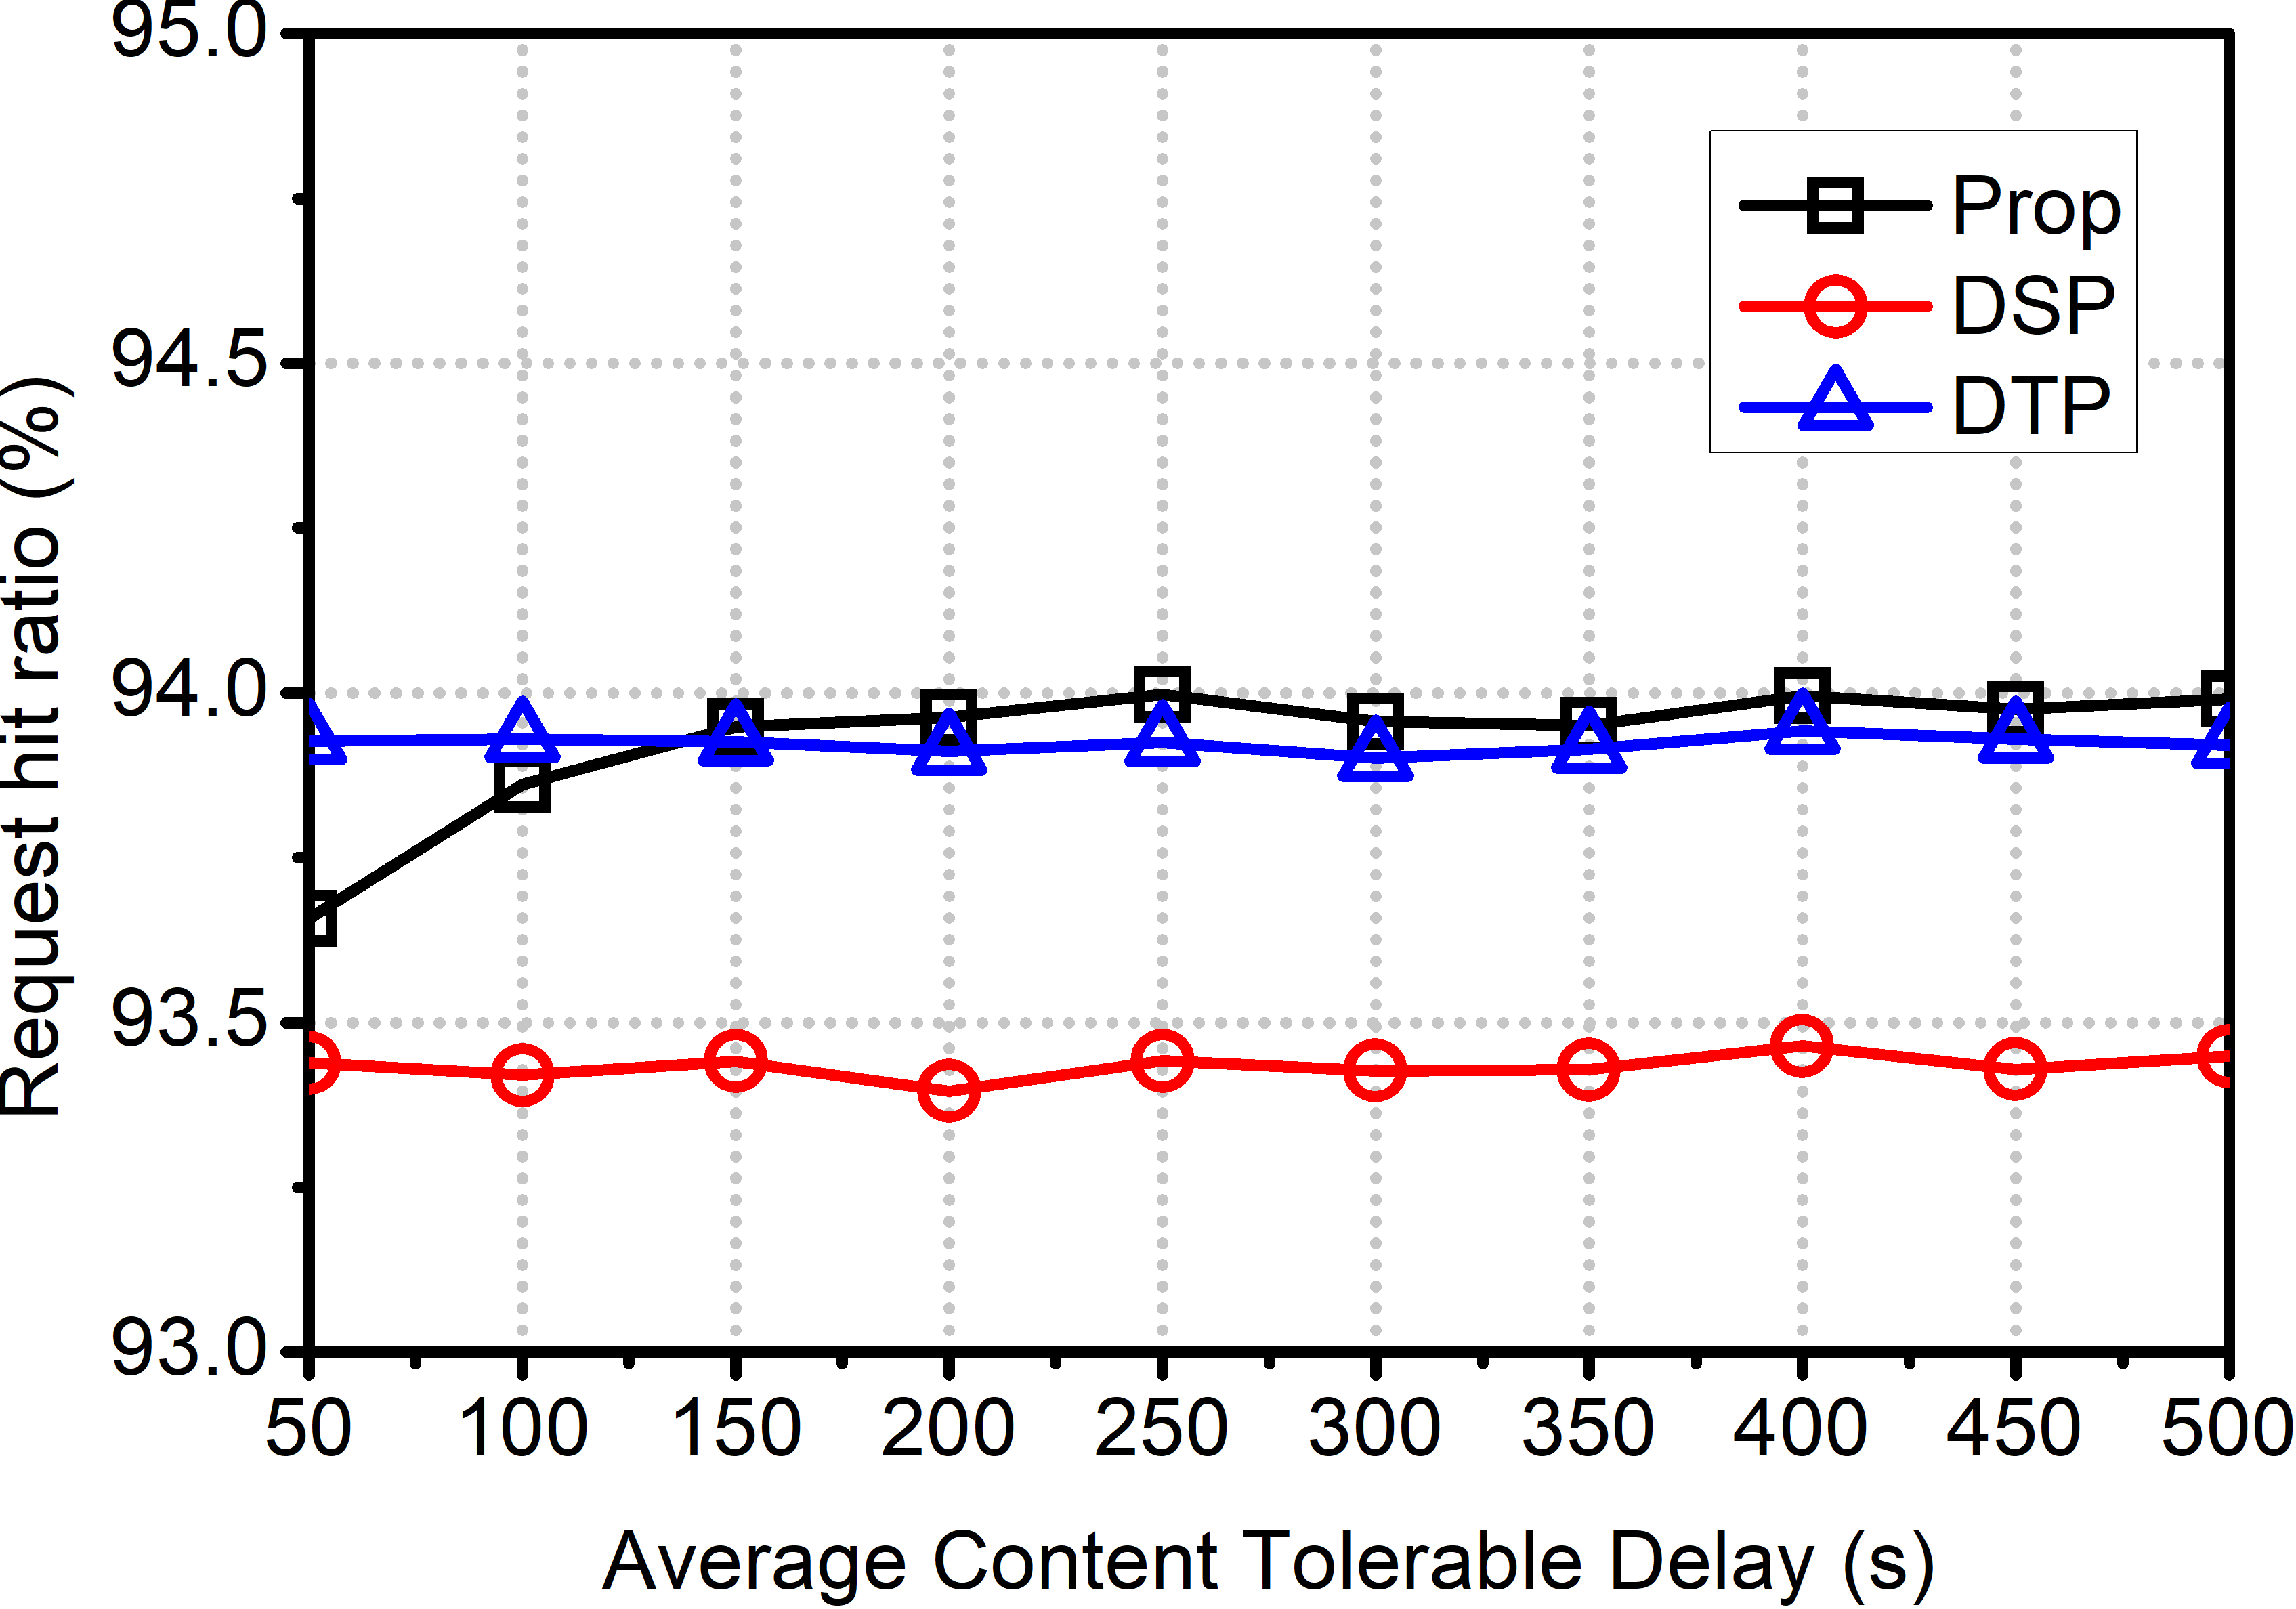
\includegraphics[width=0.325\textwidth]{./graphs/TH.png}}
    \subfigure[]{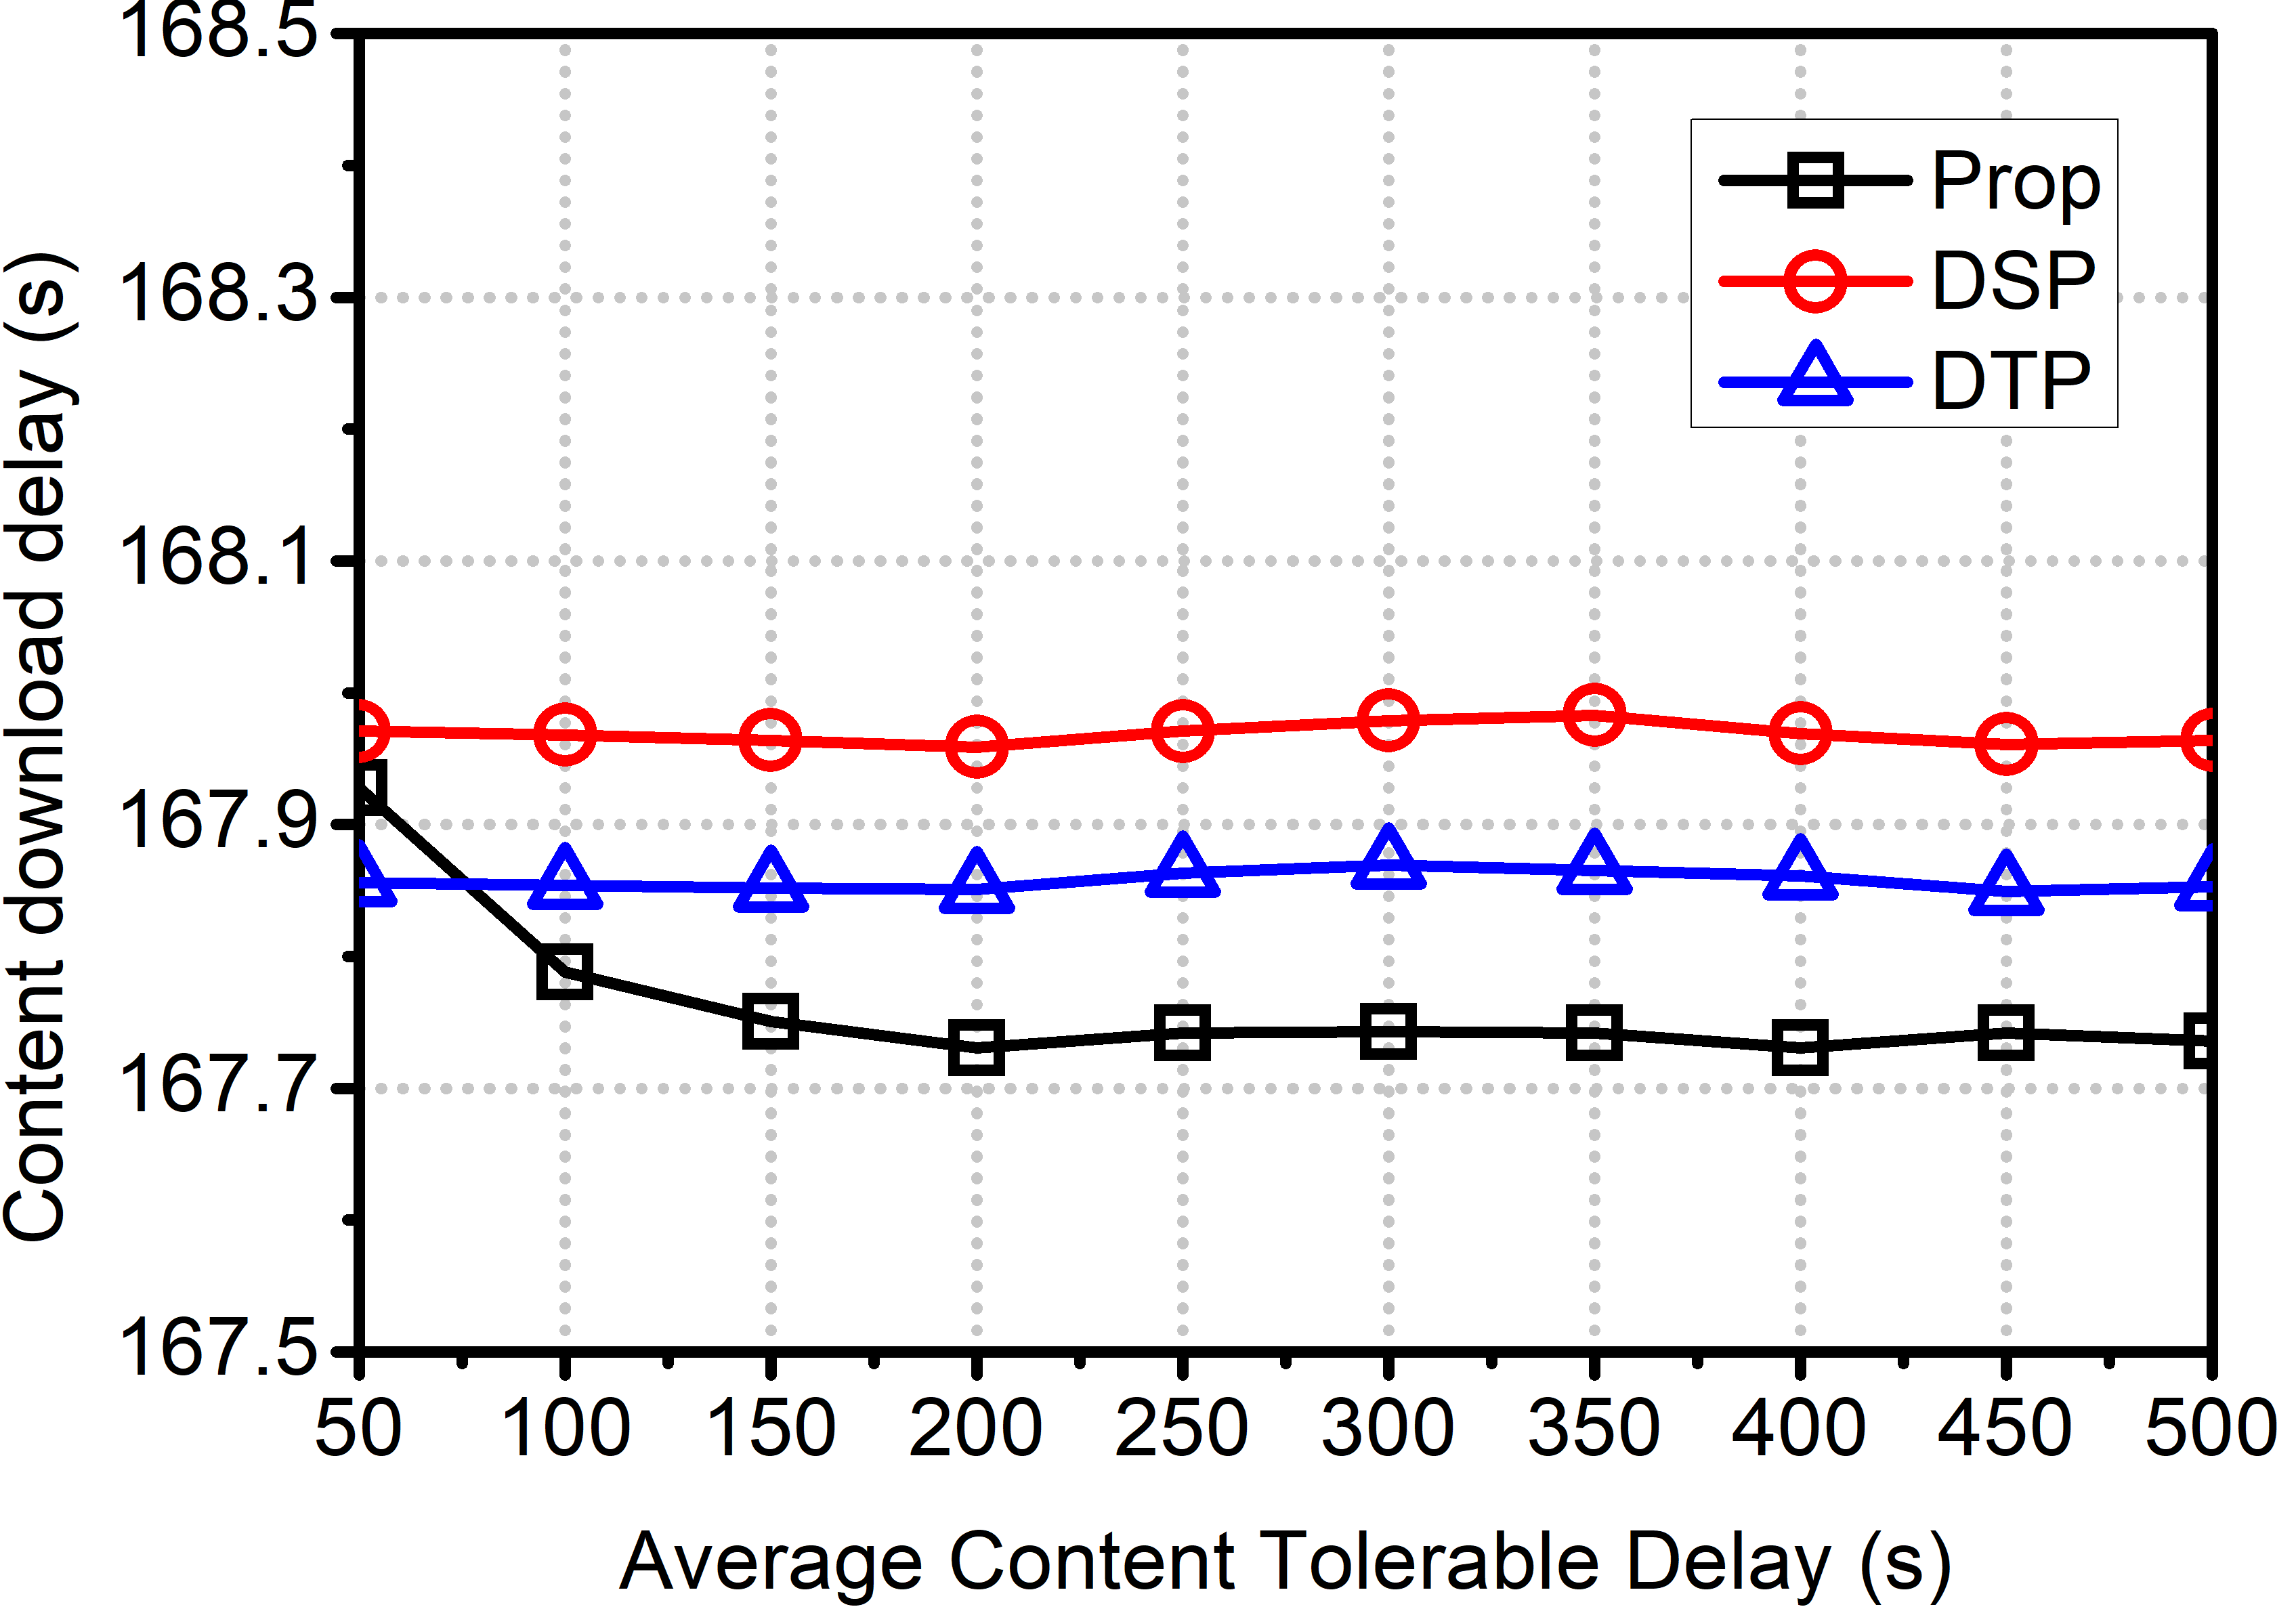
\includegraphics[width=0.325\textwidth]{./graphs/TD.png}}
    \subfigure[]{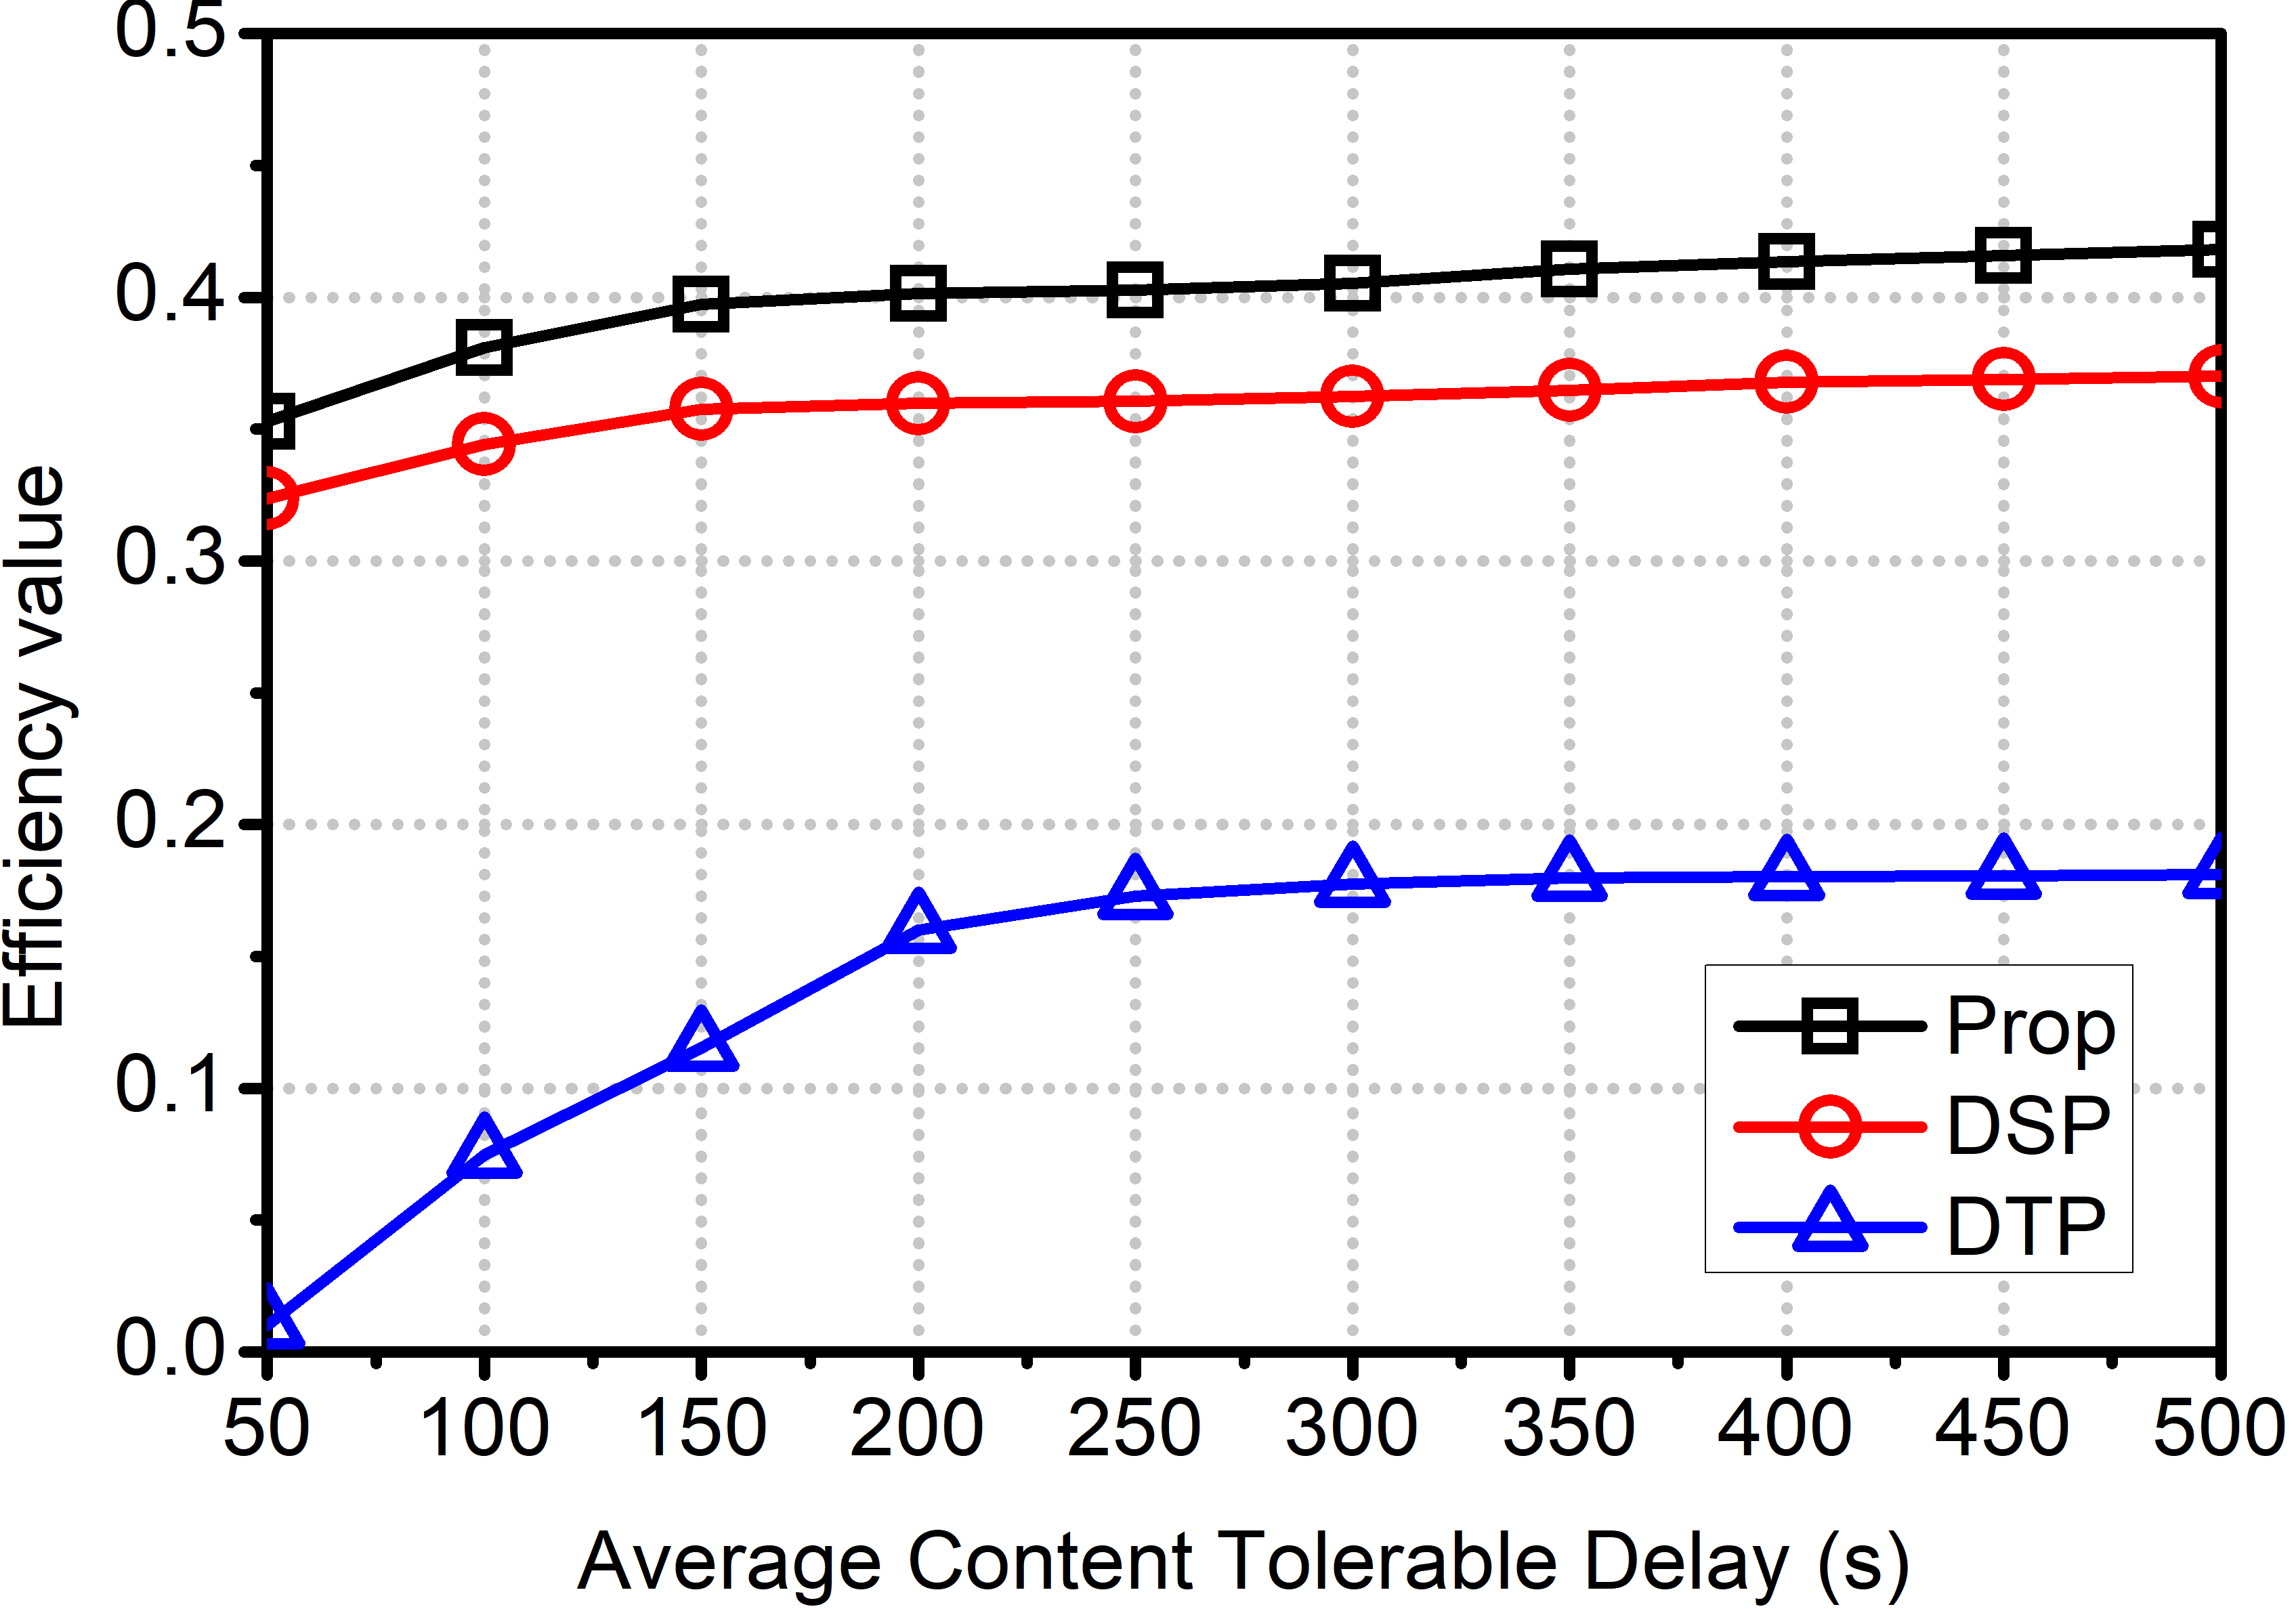
\includegraphics[width=0.325\textwidth]{./graphs/TE.png}}
    \caption{According to the average content tolerable delay: (a) request hit ratio; (b) content download delay; (c) efficiency value.}
    \label{fig:g5}
\end{figure*}

\subsubsection{Average Vehicle Speed}
Average vehicle speed is a critical evaluation parameter in assessing the performance of vehicular content delivery systems.
Since the acceleration of each vehicle is independently determined based on Gaussian distribution with a skewness, this parameter affects vehicles' movement speed within the network.
Faster vehicular mobility, resulting from a higher average speed, affects the duration of interactions between vehicles and RSUs.
Faster-moving vehicles may have shorter dwell times within an RSU's coverage area, affecting the feasibility of content precaching and the time available for content provision.
Vehicles traveling at higher speeds may spend less time within the coverage area of an RSU, which can affect the ability to precache content and the time available for providing it.
Additionally, the frequency and timing of content requests are affected by the average vehicle speed because it contributes to the overall dynamics of vehicular traffic.
A precise understanding of the average vehicle speed is essential for optimizing content provision schemes, especially in situations where vehicular mobility patterns vary, affecting the system's ability to predict and meet content delivery demands efficiently.

Figure \ref{fig:g3}(a) shows the request hit ratio according to the average vehicle speed.
Fast-moving vehicles result in less time spent within the communication range of an RSU.
This reduced dwell time reduces the likelihood that the RSU will be able to fulfill content requests, especially for DTC.
This reduced dwell time makes it difficult for the RSU to provide cached and precached chunks to vehicles before they leave the RSU's coverage area.
Therefore, faster vehicle speeds create a scenario where vehicles have less time to interact with RSUs, making it more difficult for RSUs to successfully provide content requests within the limited time, which ultimately has a negative impact on the request hit ratio.
The proposed scheme has a higher hit ratio than the other two schemes due to more accurate precaching prediction.
The DSP scheme has the lowest hit ratio due to its caching and precaching of more chunks.

Figure \ref{fig:g3}(b) shows the content download delay according to the average vehicle speed.
A shorter dwell time due to faster vehicle speeds results in less time for an RSU to predict, cache, and provide chunks, as well as for the next RSU to precache chunks.
This leads to spending more time to cache and precache the requested chunks and to predict vehicle mobility.
The speed of the vehicles has a significant impact on the turnover rate of requests in the RSU.
This results in a large amount of content being cached, precached, and erased from the caching storage.
As a result, when vehicles are traveling at high speeds, the time spent on caching and precaching chunks, as well as the time required to bring erased chunks to the RSU, causes more delays.
In DSP, reckless precaching leads to even more delays due to the need to bring the erased chunks, so DSP has the highest delay.
The proposed scheme has the lowest delay because it prevents reckless precaching in DTC and the erasure of important content.

Figure \ref{fig:g3}(c) shows the efficiency value according to the average vehicle speed.
Higher vehicle speeds result in reduced time spent within an RSU's coverage, which in turn decreases the time available for handling prediction errors for precaching, leading to a lower success ratio.
Additionally, prediction errors can cause an increase in backhaul link traffic to bring the requested chunks from other RSUs or the content server.
The efficiency value decreases due to faster vehicle speeds, caused by prediction errors and erased chunks in the caching storage of RSUs.
Specifically, since DTP does not precache the chunks of the requested DTC, the impact of prediction errors increases in terms of success ratio, resulting in the lowest efficiency value.
The proposed scheme has the highest efficiency value due to its higher prediction accuracy through recalculation compared to DSP.


\subsubsection{Average Content Size}
Average content size is an important parameter in evaluating vehicular content delivery systems as it provides insights into the characteristics of transmitted data.
This metric represents the average size of requested content from vehicles, reflecting the variety of multimedia files, software updates, or other digital assets within the network.
The size of each content is independently determined based on Gaussian distribution with this average.
Larger average content sizes can impact both the required bandwidth and the storage capacity of RSUs, affecting the efficiency of data transmission and storage.
Moreover, variations in content size can impact the duration of content delivery and retrieval, resulting in alterations to network traffic.
Understanding the average content size is essential for developing schemes related to caching, precaching, and overall content management, as it directly affects the resource utilization and responsiveness of vehicular content delivery systems.

Figure \ref{fig:g4}(a) shows the request hit ratio according to the average size of all the content.
Larger content sizes result in more erased content due to storage limitations, which can
lead to the erasure of popular cached and precached content.
As a result, requests for such content may not be hit, leading to a reduction in the request hit ratio.
In DSP, excessive precaching causes RSUs to precache more chunks, resulting in the lowest hit ratio.
The proposed scheme has a higher hit ratio for precaching than DTP, indicating its superior prediction accuracy.

Figure \ref{fig:g4}(b) shows the content download delay according to the average size of all the content.
The time required to provide content increases with its size due to the larger number of chunks.
As a result, there is a linear relationship between the size of the content and the content download delay.
Furthermore, when the storage limit of RSUs' caching storage is exceeded, erased chunks due to the increased size of the content cause further delays in bringing them back.
Reckless precaching in DSP leads to more erased chunks, resulting in additional delays.
Therefore, DSP has the highest content download delay.
The DTP and proposed scheme aim to reduce backhaul link traffic and caching storage of RSUs by considering the delay tolerance characteristics of content.
This approach can effectively reduce the number of erased chunks.
Additionally, the proposed scheme minimizes prediction errors for precaching, resulting in the shortest content download delay possible.

Figure \ref{fig:g4}(c) shows the efficiency value according to the average size of all the content.
When a large DTC size is requested, more RSUs are required for successful downloading.
However, due to the tolerable delay of the DTC, the success ratio decreases as more RSUs are needed.
Additionally, an increased size of content leads to erased chunks and a low hit ratio, resulting in a further decrease in the success ratio.
The size of the content affects the required traffic consumption on the backhaul links, and the erased chunks can increase the traffic.
As a result, larger content sizes reduce the efficiency of precaching schemes.
DTP has a low success rate because it does not precache DTC chunks, as it ignores their tolerable delay, resulting in the lowest efficiency value.
The proposed scheme is more efficient than DSP because DSP consumes a significant amount of traffic on backhaul links to precache all chunks of DTC and DSC.


\subsubsection{Average Content Tolerable Delay}
Average content tolerable delay is a critical evaluation parameter in vehicular content delivery systems.
It represents the average duration that a vehicle can endure while waiting for a requested content item.
This metric reflects the balance between the timeliness of content provision and the tolerable delay perceived by users.
A shorter average tolerable delay enhances QoS and user satisfaction, especially for delay-sensitive content.
Conversely, a higher average tolerable delay may be acceptable for delay-tolerant content, considering the diverse nature of applications in vehicular scenarios.
Striking the right balance in the Average Content Tolerable Delay is crucial for optimizing system performance, minimizing access delays, and aligning with the expectations of users who engage with both delay-sensitive and delay-tolerant content in dynamic vehicular environments.

Figure \ref{fig:g5}(a) shows the request hit ratio according to the average tolerable delay of content.
The graph shows a horizontal trend, indicating that the hit ratio is insensitive to changes in the tolerable delay of the content.
Regardless of the tolerable delay parameter, the hit ratio remains relatively constant, suggesting that variations in content tolerances do not significantly influence the hit ratio.
In this scenario, DSP has the lowest hit ratio due to lower prediction accuracy and erased chunks resulting from reckless precaching and the absence of a proper caching policy.
When comparing the two schemes that do not use reckless precaching, the proposed scheme has the highest hit ratio due to a proper precaching algorithm for DTC and improved prediction accuracy through recalculation.
However, rushing to precache DTC with a shorter tolerable delay increases backhaul link traffic, causing erased chunks and decreasing the hit ratio in the proposed scheme.

Figure \ref{fig:g5}(b) shows the content download delay according to the average tolerable delay of content.
The graph shows a horizontal trend, indicating insensitivity to changes in the tolerable delay.
This suggests that the impact of tolerable delay is minimal, resulting in consistent performance across different tolerable delay scenarios.
The delay in downloading content is affected by the hit ratio, as the requested chunks are provided by other RSUs or the content server when they are not hit.
The two comparison schemes do not take into account the tolerance characteristics of the content, but the proposed scheme does.
When the requested content has a small tolerable delay, the proposed scheme precaches almost all chunks of the content.
However, due to its proper caching policy, it has a lower content download delay than DSP and DTP.

Figure \ref{fig:g5}(c) shows the efficiency value according to the average tolerable delay of content.
If the requested content has a shorter tolerable delay, it may not be downloaded within its tolerable delay.
Therefore, DTP, which only uses the cached RSUs without precaching DTC, has the worst performance in terms of the efficiency value, even though it hardly consumes backhaul link traffic for DTC due to no precaching.
Although DSP has the highest success ratio, its efficiency value is lower than that of the proposed scheme due to reckless precaching.
The proposed scheme has the highest efficiency value because of its high success ratio and the saved traffic consumption on backhaul links due to the proper precaching algorithm for DTC.
When the tolerable delay of DTC is reduced, the proposed scheme uses more traffic to precache DTC chunks, increasing the success ratio but decreasing the efficiency value.


\section{Conclusion} \label{sec.conc}
In this paper, we proposed a comprehensive Content Storage Management and Precaching (CSMP) scheme to prevent the inadvertent erasure of content and alleviate high backhaul link traffic delays in CCN-IoV.
Initially, the CSMP scheme includes the Content Storage Management (CSM) method, which prioritizes cached content to prevent inadvertent content erasures caused by storage limitations, followed by the implementation of the Delay-Tolerant Content Precaching (DTCP) method to alleviate backhaul link traffic.
Additionally, we proposed the Delay-Sensitive Content Precaching (DSCP) method to improve mobility prediction accuracy and minimize delays in provisioning delay-sensitive content.
Moreover, to reflect various realistic scenarios, we have designed a vehicle mobility model based on a Gaussian normal distribution with skewness and a content request model based on Zipf's law, Gaussian normal distribution, and Poisson distribution.
This paper shows that, based on simulation results, the evaluation value that considers the success ratio and the backhaul link traffic improves by 23.21\% compared to the comparison delay sensitive precaching scheme, leading to reducing content download delay and enhancing the request hit ratio.
Therefore, through this approach, autonomous vehicles can conserve backhaul links without sacrificing the provision of delay-tolerant content, while efficiently prioritizing content caching, ensuring that delay-sensitive content is delivered with minimal delay in CCN-IoV.



% \appendices
% \section{Proof of the First Zonklar Equation}
% Appendix one text goes here.

% you can choose not to have a title for an appendix
% if you want by leaving the argument blank
% \section{}
% Appendix two text goes here.


% use section* for acknowledgment
% \section*{Acknowledgment}
% The authors would like to thank...


% Can use something like this to put references on a page
% by themselves when using endfloat and the captionsoff option.
\ifCLASSOPTIONcaptionsoff
  \newpage
\fi



% trigger a \newpage just before the given reference
% number - used to balance the columns on the last page
% adjust value as needed - may need to be readjusted if
% the document is modified later
%\IEEEtriggeratref{8}
% The "triggered" command can be changed if desired:
%\IEEEtriggercmd{\enlargethispage{-5in}}

% references section

% can use a bibliography generated by BibTeX as a .bbl file
% BibTeX documentation can be easily obtained at:
% http://mirror.ctan.org/biblio/bibtex/contrib/doc/
% The IEEEtran BibTeX style support page is at:
% http://www.michaelshell.org/tex/ieeetran/bibtex/
%\bibliographystyle{IEEEtran}
% argument is your BibTeX string definitions and bibliography database(s)
%\bibliography{IEEEabrv,../bib/paper}
%
% <OR> manually copy in the resultant .bbl file
% set second argument of \begin to the number of references
% (used to reserve space for the reference number labels box)
\begin{thebibliography}{999} % \linebreak

% Introduction
\bibitem{Zhe2020} Z. Zhang, C. -H. Lung, M. St-Hilaire and I. Lambadaris,  ``Smart Proactive Caching: Empower the Video Delivery for Autonomous Vehicles in ICN--Based Networks,'' \emph{IEEE Trans. Veh. Technol.}, vol. 69, no. 7, pp. 7955--7965, Jul. 2020.
\bibitem{yuan2018} Q. Yuan, H. Zhou, J. Li, Z. Liu, F. Yang and X. S. Shen,  ``Toward Efficient Content Delivery for Automated Driving Services: An Edge Computing Solution,'' \emph{IEEE Netw.}, vol. 32, no. 1, pp. 80--86, Jan.--Feb. 2018.
\bibitem{Kumer2013} V. Kumar, S. Mishra and N. Chand,  ``Applications of VANETs: Present \& Future,'' \emph{Commun. and Netw.}, vol. 5, no. 1B, pp. 12--15, Feb. 2013.
\bibitem{Pranav2019} P.K. Singh, S.K. Nandi and S. Nandi,  ``A tutorial survey on vehicular communication state of the art, and future research directions,'' \emph{Veh. Commun.}, vol. 18, pp. 100164, Aug. 2019.
\bibitem{Reichardt2002} D. Reichardt, M. Miglietta, L. Moretti, P. Morsink and W. Schulz,  ``CarTALK 2000: safe and comfortable driving based upon inter--vehicle--communication,'' \emph{Intell. Veh. Symp., 2002. IEEE}, vol. 2, pp. 545--550, Jun. 2002.
\bibitem{Yen2020} Y. -T. Yen, J. -J. Chou, C. -S. Shih, C. -W. Chen and P. -K. Tsung,  ``Proactive Car--Following Using Deep--Reinforcement Learning,'' presented at the \emph{23\textsuperscript{rd} Int. Conf. Intell. Transp. Syst.}, Rhodes, Greece, Sep. 20--23, 2020.

\bibitem{Ericsson} Ericsson Mobility Report. Available online: \url{https://www.ericsson.}
\url{com/en/reports-and-papers/mobility-report/dataforecasts/mobile-traffic}
\url{-forecast/} (Accessed: March 29, 2024).

% CCN
\bibitem{Jacobson2009} V. Jacobson, D.K. Smetters, J.D. Thornton, M.F. Plass, N.H. Briggs and R.L. Braynard,  ``Networking Named Content,'' in \emph{Proc. ACM 5th Int. Conf. Emerg. Netw. Exp. Technol.}, Rome, Italy, Dec. 2009, pp. 1--12.
\bibitem{zhang2014} L. Zhang, A. Afanasyev, J. Burke, V. Jacobson, K. Claffy, P. Crowley, C. Papadopoulos, L. Wang and B. Zhang, ``Named data networking,'' \emph{ACM SIGCOMM Comput. Commun. Rev.}, vol. 44, issue. 3 pp. 66-–73, Jul. 2014.

% CCN-IoV
\bibitem{Li2017} Z. Li, Y. Chen, D. Liu and X. Li, ``Performance analysis for an enhanced architecture of IoV via Content--Centric Networking,'' \emph{EURASIP J. Wireless Commun. Netw.}, vol. 2017, no. 1, pp. 1--7, Dec. 2017.
\bibitem{Hichri2021} Y. Hichri, S. Dahi and H. Fathallah, ``Candidate architectures for emerging IoV: a survey and comparative study,'' \emph{Des. Autom. Embed. Syst.}, vol. 25, pp. 237-–263, Aug. 2021.

% Precaching
\bibitem{Ding2022} H. Ding, Y. Ma, C. Zhang, X. Li, B. Lin, Y. Fang, and S. Chen, ``Probabilistic Data Prefetching for Data Transportation in Smart Cities,'' \emph{IEEE Internet Things J.}, vol. 9, no. 3, pp. 1655--1666, Feb. 2022.
\bibitem{Wu2022} Y. Wu, X. Fang, C. Luo and G. Min, ``Intelligent Content Precaching Scheme for Platoon--Based Edge Vehicular Networks,'' \emph{IEEE Internet Things J.}, vol. 9, no. 20, pp. 20503--20518, Oct. 2022.
\bibitem{AlNagar2022} Y. AlNagar, R. H. Gohary, S. Hosny and A. A. El-Sherif, ``Mobility--Aware Edge Caching for Minimizing Latency in Vehicular Networks,'' \emph{IEEE Open J. Veh. Technol.}, vol. 3, pp. 68--84, Feb. 2022.

\bibitem{Yu2022} S. Yu, E. Sheng, Y. Zhang, Y. Li, H. Chen and Y. Hao, ``Efficient Nonlinear Model Predictive Control of Automated Vehicles,'' \emph{Mathematics}, vol. 10, no. 21, pp. 4163, Nov. 2022.
\bibitem{Xu2020} S. Xu, C. Guo, ``Computation Offloading in a Cognitive Vehicular Networks with Vehicular Cloud Computing and Remote Cloud Computing,'' \emph{Sensors}, vol. 20, no. 23, pp. 6820, Nov. 2020.

% caching storage in Precaching
\bibitem{Lin2021} L. Yao, Y. Wang, X. Wang and G. WU,  ``Cooperative Caching in Vehicular Content Centric Network Based on Social Attributes and Mobility,'' \emph{IEEE Trans. Mob. Comput.},  vol. 20, no. 2, pp. 391--402, Feb. 2021.
\bibitem{Yao2018} L. Yao, A. Chen, J. Deng, J. Wang and G. Wu,  ``A Cooperative Caching Scheme Based on Mobility Prediction in Vehicular Content Centric Networks,'' \emph{IEEE Trans. Veh. Technol.}, vol. 67, no. 6, pp. 5435--5444, Jun. 2018.
\bibitem{Wang2021} R. Wang, Z. Kan, Y. Cui, D. Wu and Y. Zhen,  ``Cooperative Caching Strategy With Content Request Prediction in Internet of Vehicles,'' \emph{IEEE Internet Things J.}, vol. 8, no. 11, pp. 8964--8975, Jun. 2021.

\bibitem{Feng2023}
B. Feng, C. Feng, D. Feng, Y. Wu and X. -G. Xia, ``Proactive Content Caching Scheme in Urban Vehicular Networks,'' \emph{IEEE Trans. Commun.}, vol. 71, no. 7, pp. 4165-4180, July 2023.
\bibitem{Liu2018} W. Liu, Y. Jiang, S. Xu, G. Cao, W. Du and Y. Cheng, ``Mobility--Aware Video Prefetch Caching and Replacement Strategies in Mobile--Edge Computing Networks,'' in \emph{Proc. IEEE 24th Int. Conf. Parallel Distrib. Syst. (ICPADS)}, Singapore, Dec. 2018, pp. 687--694.

% CCN-IoV RW
\bibitem{Amadeo2012} M. Amadeo, C. Campolo and A. Molinaro, ``Content--centric vehicular networking: An evaluation study,'' in \emph{Proc. Int. Conf. Netw. Future (NOF)}, Tunis, Tunisia, Nov. 2012, pp. 1--5.
\bibitem{Su2017} Z. Su, Y. Hui and Q. Yang,  ``The Next Generation Vehicular Networks: A Content-Centric Framework,'' \emph{IEEE Wirel. Commun.}, vol. 24, no. 1, pp. 60--66, Feb. 2017.
\bibitem{Wang2019}X. Wang and X. Wang, ``Vehicular Content--Centric Networking Framework,'' \emph{IEEE Syst. J.}, vol. 13, no. 1, pp. 519--529, Mar. 2019.

% Precaching in CCN-IoV
\bibitem{Ostrovskaya2018} S. Ostrovskaya, O. Surnin, R. Hussain, S. H. Bouk, J.Y. Lee, N. Mehran, S. H. Ahmed and A. Benslimane, ``Towards Multi--metric Cache Replacement Policies in Vehicular Named Data Networks,'' in \emph{Proc. IEEE Int. Symp. Pers. Indoor Mobile Radio Commun. (PIMRC)}, Bologna, Italy, Sep. 2018, pp. 1--7.
\bibitem{Amadeo2021} M. Amadeo, G. Ruggeri, C. Campolo and A. Molinaro, ``Diversity--improved caching of popular transient contents in Vehicular Named Data Networking,'' \emph{Comput. Netw.}, vol. 184, pp. 107625, Jan. 2021.
\bibitem{Dua2019} A. Dua, M. Shishodia, N. Kumar, G.S. Aujla and N. Kumar, ``Bloom Filter Based Efficient Caching Scheme for Content Distribution in Vehicular Networks,'' in \emph{Proc. IEEE 17th Int. Conf. Commun. Workshops (ICC Workshops)}, Shanghai, China, May 2019, pp. 20--24.

% Precaching RW
\bibitem{Park2019} S. Park, S. Oh, Y. Nam, J. Bang and E. Lee,  ``Mobility--aware Distributed Proactive Caching in Content--Centric Vehicular Networks,'' in \emph{Proc. 12th IFIP Wireless Mobile Netw. Conf.}, Paris, France, Sep. 2019, pp. 175--180.
\bibitem{Ahani2018} G. Ahani and D. Yuan, ``On Optimal Proactive and Retention-Aware Caching with User Mobility,'' in \emph{Proc. IEEE 88th Veh. Technol. Conf. (VTC-Fall)}, Chicago, IL, USA, Nov. 2018, pp. 1--5.
\bibitem{AlNagar2019} Y. AlNagar, S. Hosny and A. A. El-Sherif, ``Towards Mobility--Aware Proactive Caching for Vehicular Ad hoc Networks,'' in \emph{Proc. IEEE Wireless Commun. Netw. Conf. Workshop (WCNCW)}, Marrakech, Morocco, Apr. 2019, pp. 1--6.
\bibitem{Liang2018} C. Liang, F. R. Yu, N. Dao, G. Senarath and H. Farmanbar, ``Enabling Adaptive Data Prefetching in 5G Mobile Networks with Edge Caching,'' in \emph{Proc. IEEE Conf. Global Commun. (GLOBECOM)}, Abu Dhabi, United Arab Emirates, Dec. 2018, pp. 1--6.

\bibitem{Ikram2021} I. Ud Din, B. Ahmad, A. Almogren, H. Almajed, I. Mohiuddin and J. J. P. C. Rodrigues,  ``Left--Right--Front Caching Strategy for Vehicular Networks in ICN--Based Internet of Things,'' \textit{IEEE Access}, vol. 9, pp. 595--605, Dec. 2021.
\bibitem{Zhao2023} W. Zhao, C. Wu, R. Zhong, K. Shi and X. Xu, ``Edge Computing and Caching Optimization Based on PPO for Task Offloading in RSU--Assisted IoV,’’ in \emph{Proc. IEEE 9th World Forum on Internet of Things (WF--IoT)}, Aveiro, Portugal, Oct. 2023, pp. 01--06.

\bibitem{Khan2024} M. T. R. Khan, Y. Z. Jembre, M. M. Saad, S. H. Bouk, S. H. Ahmed and D. Kim, ``Proactive Content Retrieval Based on Value of Popularity in Content--Centric Internet of Vehicles,'' \emph{IEEE Trans. Intell. Transp. Syst.}, vol. 25, no. 8, pp. 8514--8526, Aug. 2024.

\bibitem{Grewe2018} D. Grewe, S. Schildt, M. Wagner and H. Frey, ``ADePt: Adaptive Distributed Content Prefetching for Information--Centric Connected Vehicles,'' in \emph{Proc. IEEE 87th Veh. Technol. Conf. (VTC Spring)}, Porto, Portugal, Jun. 2018, pp. 1--5.
\bibitem{Zhang2015} F. Zhang, X. Chenren, Y. Zhang, K. K. Ramakrishnan, S. Mukherjee, R. Yates, and N. Thu, ``EdgeBuffer: Caching and prefetching content at the edge in the MobilityFirst future Internet architecture,'' in \emph{Proc. 16th Int. Symp. World Wireless Mobile Multimedia Netw. (WoWMoM)}, Boston, MA, USA, Jun. 2015, pp. 1--9.

% DTN RW
\bibitem{Vigneri2019} L. Vigneri, T. Spyropoulos and C. Barakat ``Low Cost Video Streaming through Mobile Edge Caching: Modelling and Optimization,'' \emph{IEEE Trans. Mob. Comput.}, vol. 18, no. 6, pp. 1302--1315, Jun. 2019.
\bibitem{Prates2019} A. A. Prates, I. V. Bastos and I. M. Moraes, ``GeoZone: An interest--packet forwarding mechanism based on dissemination zone for content--centric vehicular networks,'' \emph{Comput. \& Electr. Eng.}, vol. 73, pp. 155--166, Jan. 2019.
\bibitem{Aung2023} N. Aung, S. Dhelim, L. Chen, A. Lakas, W. Zhang, H. Ning, S. Chaib and M. T. Kechadi, ``VeSoNet: Traffic-Aware Content Caching for Vehicular Social Networks Using Deep Reinforcement Learning,'' \emph{IEEE Trans. Intell. Transp. Syst.}, vol. 24, no. 8, pp. 8638--8649, Aug. 2023.

\bibitem{Wang2018} R. Wang, A. Sabbagh, S. C. Burleigh, K. Zhao and Y. Qian, ``Proactive Retransmission in Delay--/Disruption--Tolerant Networking for Reliable Deep--Space Vehicle Communications,'' \emph{IEEE Trans. Veh. Technol.}, vol. 67, no. 10, pp. 9983--9994, Oct. 2018.
\bibitem{Qi2017} W. Qi, Q. Song, X. Wang and L. Guo, ``Trajectory Data Mining--Based Routing in DTN--Enabled Vehicular Ad Hoc Networks,'' \emph{IEEE Access}, vol. 5, pp. 24128--24138, Oct. 2017.
\bibitem{Xia2020} B. Xia, F. Kong, J. Zhou, X. Tang and H. Gong, ``A Delay--Tolerant Data Transmission Scheme for Internet of Vehicles Based on Software Defined Cloud-Fog Networks,'' \emph{IEEE Access}, vol. 8, pp. 65911--65922, Mar. 2020.

\bibitem{WAVE} A. Paier, R. Tresch, A. Alonso, D. Smely, P. Meckel, Y. Zhou and N. Czink, ``Average Downstream Performance of Measured IEEE 802.11p Infrastructure-to-Vehicle Links,'' \emph{Proc. IEEE Int. Conf. Commun. Workshops (ICC Workshops)}, Cape Town, South Africa, May 2010, pp. 1--5.
\bibitem{Lee2014} E. Lee, E. Lee, M. Gerla and S. Y. Oh,  ``Vehicular cloud networking: architecture and design principles,'' \emph{IEEE Comm. Magazine}, vol. 52, no. 2, pp. 148--155, Feb. 2014.
\bibitem{Chen2009} B. B. Chen and M. C. Chan,  ``MobTorrent: A Framework for Mobile Internet Access from Vehicles,'' \emph{IEEE INFOCOM}, Rio de Janeiro, Brazil, Apr. 2009, pp. 1404--1412.

\bibitem{Azzalini} A. Azzalini and A. Capitanio, ``The Skew--Normal and Related Families,'' \emph{Cambridge University Press}, 2013.
\bibitem{Zipf} L. Breslau, Pei Cao, Li Fan, G. Phillips and S. Shenker, ``Web caching and Zipf--like distributions: evidence and implications,'' in \emph{Proc. IEEE INFOCOM}, New York, NY, USA, Mar. 1999, pp. 126--134.
\bibitem{NS3} Network Simulator 3 (NS3). [Online]. Available: \url{https://www.nsnam.} \url{org/} (Accessed: March 29, 2024).
\bibitem{Manhattan}
A. Hanggoro and R. F. Sari, ``Performance evaluation of the manhattan mobility model in vehicular ad-hoc networks for high mobility vehicle,'' in \emph{Proc. IEEE Int. Conf. Commun. Netw. Satellite (COMNETSAT)}, Yogyakarta, Indonesia, Dec. 2013, pp. 31--36.

\end{thebibliography}

% biography section
% 
% If you have an EPS/PDF photo (graphicx package needed) extra braces are
% needed around the contents of the optional argument to biography to prevent
% the LaTeX parser from getting confused when it sees the complicated
% \includegraphics command within an optional argument. (You could create
% your own custom macro containing the \includegraphics command to make things
% simpler here.)
%\begin{IEEEbiography}[{\includegraphics[width=1in,height=1.25in,clip,keepaspectratio]{mshell}}]{Michael Shell}
% or if you just want to reserve a space for a photo:

\begin{IEEEbiography}[{
\includegraphics[width=1in,height=1.25in,clip,keepaspectratio]{./photo/YoungjuNam.jpg}}]
{Youngju Nam} received the B.S., M.S., and Ph.D. degrees from the School of Information and Communication Engineering, Chungbuk National University, Cheongju, South Korea, in 2017, 2019, and 2023, respectively. He is currently researching with the Research Institute for Computer and Information Communication, Chungbuk National University. His research interests include computer communication and networking, wireless sensor networks, content-centric vehicular networks, content precaching, optimization, and social networks.
\end{IEEEbiography}

\begin{IEEEbiography}[{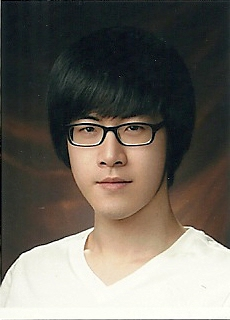
\includegraphics[width=1in,height=1.25in,clip,keepaspectratio]{./photo/HyunseokChoi.jpg}}]
{Hyunseok Choi} received the B.S. and Ph.D. degrees from the School of Information and Communication Engineering, Chungbuk National University, Cheongju, South Korea, in 2017 and 2023. He is currently researching with the Research Institute for Computer and Information Communication, Chungbuk National University. His research interests include computer communication and networking, wireless sensor networks, vehicular ad-hoc networks, vehicular clustering, and cloud computing.
\end{IEEEbiography}

\begin{IEEEbiography}[{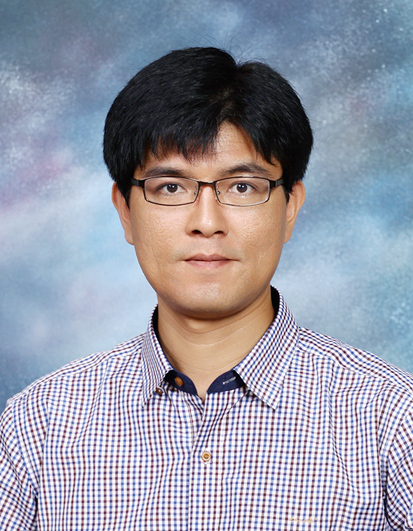
\includegraphics[width=1in,height=1.25in,clip,keepaspectratio]{./photo/EuisinLee.jpg}}]
{Euisin Lee} received the B.S., M.S., and Ph.D. degrees in computer engineering from Chungnam National University, Daejeon, South Korea, in 2005, 2007, and 2012, respectively. He studied as a Postdoctoral Researcher with the Department of Computer Science, University of California at Los Angeles, from 2012 to 2014. He joined the School of Information and Communication Engineering, Chungbuk National University, in 2014, where he is currently working as a Professor. His research interests include computer communication and networking, routing, multicasting, mobility management, location service, QoS (real-time and reliability) in mobile ad hoc networks (MANETs), wireless sensor networks (WSNs), vehicular ad hoc networks (VANETs), Internet of Things (IoT), and Information-Centric Networking (ICN). 
\end{IEEEbiography}

% insert where needed to balance the two columns on the last page with
% biographies
%\newpage


% You can push biographies down or up by placing
% a \vfill before or after them. The appropriate
% use of \vfill depends on what kind of text is
% on the last page and whether or not the columns
% are being equalized.

%\vfill

% Can be used to pull up biographies so that the bottom of the last one
% is flush with the other column.
%\enlargethispage{-5in}


% that's all folks
\end{document}


